%% Supplementary material for the Computers in Biology and Medicine submission. Numbers are
%% \pn{key} look-ups into numbers.tex (src/paper_numbers.py); tables are generated by
%% src/paper_supp_tex.py and src/paper_tables_tex.py.
\documentclass[11pt]{article}
\usepackage[a4paper,margin=2.2cm]{geometry}
\usepackage{graphicx,booktabs,amsmath,amssymb,array,longtable}
\usepackage[T1]{fontenc}
\usepackage{lmodern}
\usepackage{textcomp}
\usepackage{xurl}
\usepackage[hidelinks]{hyperref}
\usepackage{caption}
\captionsetup{font=small,labelfont=bf}
\renewcommand{\thetable}{S\arabic{table}}
\renewcommand{\thefigure}{S\arabic{figure}}

\makeatletter
\newcommand{\pndef}[2]{\expandafter\def\csname pn@#1\endcsname{#2}}
\newcommand{\pn}[1]{\ifcsname pn@#1\endcsname\csname pn@#1\endcsname\else
  \@latex@error{Undefined number key `#1'}{Run src/paper_numbers.py}\textbf{??#1??}\fi}
\makeatother
% GENERATED by src/paper_numbers.py -- do not edit by hand.
\pndef{aptos.R1.mean.max}{+0.26}
\pndef{aptos.R1.mean.min}{+0.14}
\pndef{aptos.R1.mild.max}{14.3}
\pndef{aptos.R1.mild.min}{1.6}
\pndef{aptos.R1.qwk.max}{0.9026}
\pndef{aptos.R1.qwk.min}{0.8623}
\pndef{aptos.R1.sens.max}{99.5}
\pndef{aptos.R1.sens.min}{98.2}
\pndef{aptos.R1.spec.max}{85.3}
\pndef{aptos.R1.spec.min}{83.9}
\pndef{aptos.R2.mild.max}{22.7}
\pndef{aptos.R2.mild.min}{5.7}
\pndef{aptos.R2.qwk.max}{0.9000}
\pndef{aptos.R2.qwk.min}{0.8603}
\pndef{aptos.R2.sens.max}{99.1}
\pndef{aptos.R2.sens.min}{96.3}
\pndef{aptos.R3.mild.max}{7.0}
\pndef{aptos.R3.mild.min}{1.4}
\pndef{aptos.R3.qwk.max}{0.9000}
\pndef{aptos.R3.qwk.min}{0.8470}
\pndef{aptos.R3.sens.max}{99.7}
\pndef{aptos.R3.sens.min}{99.1}
\pndef{aptos.R4.mean.max}{+0.08}
\pndef{aptos.R4.mean.min}{+0.03}
\pndef{aptos.R4.mild.max}{18.6}
\pndef{aptos.R4.mild.min}{10.0}
\pndef{aptos.R4.qwk.max}{0.9067}
\pndef{aptos.R4.qwk.min}{0.8868}
\pndef{aptos.R4.sens.max}{98.6}
\pndef{aptos.R4.sens.min}{96.3}
\pndef{aptos.R4.spec.max}{87.1}
\pndef{aptos.R4.spec.min}{85.7}
\pndef{aptos.R4m.mild.max}{77.8}
\pndef{aptos.R4m.mild.min}{61.6}
\pndef{aptos.R4m.qwk.max}{0.8896}
\pndef{aptos.R4m.qwk.min}{0.8574}
\pndef{aptos.R4m.sens.max}{81.1}
\pndef{aptos.R4m.sens.min}{71.2}
\pndef{aptos.auroc.max}{0.973}
\pndef{aptos.auroc.min}{0.914}
\pndef{aptos.band.e08.miss.hi}{156}
\pndef{aptos.band.e08.miss.lo}{4}
\pndef{aptos.band.e08.nref}{1,487}
\pndef{aptos.band.e08.qwkmax}{0.9075}
\pndef{aptos.band.e08.sens.hi}{99.7}
\pndef{aptos.band.e08.sens.lo}{89.5}
\pndef{aptos.band.e08.spec.hi}{91.0}
\pndef{aptos.band.e08.spec.lo}{82.3}
\pndef{aptos.band.e10.miss.hi}{204}
\pndef{aptos.band.e10.miss.lo}{5}
\pndef{aptos.band.e10.nref}{1,487}
\pndef{aptos.band.e10.qwkmax}{0.9018}
\pndef{aptos.band.e10.sens.hi}{99.7}
\pndef{aptos.band.e10.sens.lo}{86.3}
\pndef{aptos.band.e10.spec.hi}{92.2}
\pndef{aptos.band.e10.spec.lo}{81.7}
\pndef{aptos.band.e11full.miss.hi}{182}
\pndef{aptos.band.e11full.miss.lo}{6}
\pndef{aptos.band.e11full.nref}{1,487}
\pndef{aptos.band.e11full.qwkmax}{0.9103}
\pndef{aptos.band.e11full.sens.hi}{99.6}
\pndef{aptos.band.e11full.sens.lo}{87.8}
\pndef{aptos.band.e11full.spec.hi}{92.3}
\pndef{aptos.band.e11full.spec.lo}{82.3}
\pndef{aptos.devmild.max}{62.0}
\pndef{aptos.devmild.min}{26.8}
\pndef{aptos.e08.R1.mild}{5.9}
\pndef{aptos.e08.R1.qwk}{0.8968}
\pndef{aptos.e08.R1.sens}{99.53}
\pndef{aptos.e08.R1.spec}{84.28}
\pndef{aptos.e08.R2.mild}{8.9}
\pndef{aptos.e08.R2.qwk}{0.8827}
\pndef{aptos.e08.R2.sens}{99.13}
\pndef{aptos.e08.R2.spec}{85.06}
\pndef{aptos.e08.R3.mild}{4.6}
\pndef{aptos.e08.R3.qwk}{0.8816}
\pndef{aptos.e08.R3.sens}{99.33}
\pndef{aptos.e08.R3.spec}{84.18}
\pndef{aptos.e08.R4.mild}{18.1}
\pndef{aptos.e08.R4.qwk}{0.9036}
\pndef{aptos.e08.R4.sens}{96.64}
\pndef{aptos.e08.R4.spec}{87.03}
\pndef{aptos.e08.R4m.mild}{70.8}
\pndef{aptos.e08.R4m.qwk}{0.8858}
\pndef{aptos.e08.R4m.sens}{80.36}
\pndef{aptos.e08.R4m.spec}{95.36}
\pndef{aptos.e11full.R1.mild}{4.9}
\pndef{aptos.e11full.R1.qwk}{0.9026}
\pndef{aptos.e11full.R1.sens}{99.26}
\pndef{aptos.e11full.R1.spec}{84.32}
\pndef{aptos.e11full.R2.mild}{7.6}
\pndef{aptos.e11full.R2.qwk}{0.9000}
\pndef{aptos.e11full.R2.sens}{98.99}
\pndef{aptos.e11full.R2.spec}{84.92}
\pndef{aptos.e11full.R3.mild}{7.0}
\pndef{aptos.e11full.R3.qwk}{0.9000}
\pndef{aptos.e11full.R3.sens}{99.06}
\pndef{aptos.e11full.R3.spec}{84.83}
\pndef{aptos.e11full.R4.mild}{16.8}
\pndef{aptos.e11full.R4.qwk}{0.9067}
\pndef{aptos.e11full.R4.sens}{96.50}
\pndef{aptos.e11full.R4.spec}{86.57}
\pndef{aptos.e11full.R4m.mild}{75.1}
\pndef{aptos.e11full.R4m.qwk}{0.8896}
\pndef{aptos.e11full.R4m.sens}{75.25}
\pndef{aptos.e11full.R4m.spec}{96.41}
\pndef{aptos.nmodels}{10}
\pndef{aptos.o7.mildrecall.between}{12.7}
\pndef{aptos.o7.mildrecall.holds}{was falsified}
\pndef{aptos.o7.mildrecall.within}{5.7}
\pndef{aptos.o7.nfail}{2}
\pndef{aptos.o7.qwk.between}{0.0404}
\pndef{aptos.o7.qwk.holds}{was falsified}
\pndef{aptos.o7.qwk.within}{0.0064}
\pndef{aptos.o7.refsens.between}{1.3}
\pndef{aptos.o7.refsens.holds}{was falsified}
\pndef{aptos.o7.refsens.within}{0.9}
\pndef{aptos.r2worse}{9}
\pndef{aptos.rho.R1vsR2}{0.70}
\pndef{aptos.rho.R1vsR3}{0.70}
\pndef{aptos.rho.R1vsR4}{0.48}
\pndef{aptos.rho.R2vsR3}{1.00}
\pndef{aptos.rho.devmatchedvsR1}{0.42}
\pndef{aptos.rho.devmatchedvsR4}{0.47}
\pndef{aptos.sel.R1.mean}{+0.15}
\pndef{aptos.sel.R1.mild}{4.9}
\pndef{aptos.sel.R1.qwk}{0.9026}
\pndef{aptos.sel.R1.sens}{99.26}
\pndef{aptos.sel.R1.spec}{84.32}
\pndef{aptos.sel.R2.mean}{+0.19}
\pndef{aptos.sel.R2.mild}{7.6}
\pndef{aptos.sel.R2.qwk}{0.9000}
\pndef{aptos.sel.R2.sens}{98.99}
\pndef{aptos.sel.R2.spec}{84.92}
\pndef{aptos.sel.R3.mean}{+0.19}
\pndef{aptos.sel.R3.mild}{7.0}
\pndef{aptos.sel.R3.qwk}{0.9000}
\pndef{aptos.sel.R3.sens}{99.06}
\pndef{aptos.sel.R3.spec}{84.83}
\pndef{aptos.sel.R4.mean}{+0.03}
\pndef{aptos.sel.R4.mild}{16.8}
\pndef{aptos.sel.R4.qwk}{0.9067}
\pndef{aptos.sel.R4.sens}{96.50}
\pndef{aptos.sel.R4.spec}{86.57}
\pndef{aptos.sel.R4m.mean}{\textminus{}0.03}
\pndef{aptos.sel.R4m.mild}{75.1}
\pndef{aptos.sel.R4m.qwk}{0.8896}
\pndef{aptos.sel.R4m.sens}{75.25}
\pndef{aptos.sel.R4m.spec}{96.41}
\pndef{aptos.sel.auroc}{0.947}
\pndef{aptos.sel.brier}{0.085}
\pndef{aptos.sel.ece}{0.086}
\pndef{aptos.tr.e08.A.gap}{+18.1}
\pndef{aptos.tr.e08.A.sens}{98.12}
\pndef{aptos.tr.e08.A.spec}{86.30}
\pndef{aptos.tr.e08.A.target}{80.0}
\pndef{aptos.tr.e08.B.gap}{+14.3}
\pndef{aptos.tr.e08.B.sens}{99.33}
\pndef{aptos.tr.e08.B.spec}{84.74}
\pndef{aptos.tr.e08.B.target}{85.0}
\pndef{aptos.tr.e08.Bs.gap}{+12.3}
\pndef{aptos.tr.e08.Bs.sens}{99.53}
\pndef{aptos.tr.e08.Bs.spec}{84.23}
\pndef{aptos.tr.e08.Bs.target}{87.2}
\pndef{aptos.tr.e08.C.gap}{+4.4}
\pndef{aptos.tr.e08.C.sens}{99.93}
\pndef{aptos.tr.e08.C.spec}{79.86}
\pndef{aptos.tr.e08.C.target}{95.5}
\pndef{aptos.tr.e10.A.gap}{+17.1}
\pndef{aptos.tr.e10.A.sens}{97.11}
\pndef{aptos.tr.e10.A.spec}{86.39}
\pndef{aptos.tr.e10.A.target}{80.0}
\pndef{aptos.tr.e10.B.gap}{+13.9}
\pndef{aptos.tr.e10.B.sens}{98.86}
\pndef{aptos.tr.e10.B.spec}{84.92}
\pndef{aptos.tr.e10.B.target}{85.0}
\pndef{aptos.tr.e10.Bs.gap}{+12.2}
\pndef{aptos.tr.e10.Bs.sens}{99.39}
\pndef{aptos.tr.e10.Bs.spec}{83.86}
\pndef{aptos.tr.e10.Bs.target}{87.2}
\pndef{aptos.tr.e10.C.gap}{+4.4}
\pndef{aptos.tr.e10.C.sens}{99.87}
\pndef{aptos.tr.e10.C.spec}{78.85}
\pndef{aptos.tr.e10.C.target}{95.5}
\pndef{aptos.tr.e11full.A.gap}{+15.4}
\pndef{aptos.tr.e11full.A.sens}{95.43}
\pndef{aptos.tr.e11full.A.spec}{87.54}
\pndef{aptos.tr.e11full.A.target}{80.0}
\pndef{aptos.tr.e11full.B.gap}{+12.6}
\pndef{aptos.tr.e11full.B.sens}{97.65}
\pndef{aptos.tr.e11full.B.spec}{86.02}
\pndef{aptos.tr.e11full.B.target}{85.0}
\pndef{aptos.tr.e11full.Bs.gap}{+11.6}
\pndef{aptos.tr.e11full.Bs.sens}{98.79}
\pndef{aptos.tr.e11full.Bs.spec}{85.24}
\pndef{aptos.tr.e11full.Bs.target}{87.2}
\pndef{aptos.tr.e11full.C.gap}{+4.3}
\pndef{aptos.tr.e11full.C.sens}{99.80}
\pndef{aptos.tr.e11full.C.spec}{82.67}
\pndef{aptos.tr.e11full.C.target}{95.5}
\pndef{corn.archived.ci}{[\textminus{}0.0656, \textminus{}0.0325]}
\pndef{corn.archived.diff}{\textminus{}0.0479}
\pndef{corn.archived.qwk}{0.8168}
\pndef{ddr.R1.mean.max}{\textminus{}0.17}
\pndef{ddr.R1.mean.min}{\textminus{}0.35}
\pndef{ddr.R1.mild.max}{45.2}
\pndef{ddr.R1.mild.min}{20.5}
\pndef{ddr.R1.qwk.max}{0.7641}
\pndef{ddr.R1.qwk.min}{0.6970}
\pndef{ddr.R1.sens.max}{70.3}
\pndef{ddr.R1.sens.min}{58.9}
\pndef{ddr.R1.spec.max}{98.9}
\pndef{ddr.R1.spec.min}{97.3}
\pndef{ddr.R2.mild.max}{33.8}
\pndef{ddr.R2.mild.min}{19.5}
\pndef{ddr.R2.qwk.max}{0.7645}
\pndef{ddr.R2.qwk.min}{0.7013}
\pndef{ddr.R2.sens.max}{65.2}
\pndef{ddr.R2.sens.min}{50.4}
\pndef{ddr.R3.mild.max}{26.5}
\pndef{ddr.R3.mild.min}{8.7}
\pndef{ddr.R3.qwk.max}{0.7723}
\pndef{ddr.R3.qwk.min}{0.7259}
\pndef{ddr.R3.sens.max}{72.1}
\pndef{ddr.R3.sens.min}{65.0}
\pndef{ddr.R4.mean.max}{+0.01}
\pndef{ddr.R4.mean.min}{\textminus{}0.03}
\pndef{ddr.R4.mild.max}{41.4}
\pndef{ddr.R4.mild.min}{22.7}
\pndef{ddr.R4.qwk.max}{0.8131}
\pndef{ddr.R4.qwk.min}{0.7467}
\pndef{ddr.R4.sens.max}{81.2}
\pndef{ddr.R4.sens.min}{70.0}
\pndef{ddr.R4.spec.max}{96.3}
\pndef{ddr.R4.spec.min}{92.6}
\pndef{ddr.R4m.mild.max}{62.1}
\pndef{ddr.R4m.mild.min}{51.6}
\pndef{ddr.R4m.qwk.max}{0.7993}
\pndef{ddr.R4m.qwk.min}{0.7377}
\pndef{ddr.R4m.sens.max}{69.4}
\pndef{ddr.R4m.sens.min}{63.2}
\pndef{ddr.auroc.max}{0.955}
\pndef{ddr.auroc.min}{0.921}
\pndef{ddr.band.e08.miss.hi}{1,681}
\pndef{ddr.band.e08.miss.lo}{766}
\pndef{ddr.band.e08.nref}{5,626}
\pndef{ddr.band.e08.qwkmax}{0.8068}
\pndef{ddr.band.e08.sens.hi}{86.4}
\pndef{ddr.band.e08.sens.lo}{70.1}
\pndef{ddr.band.e08.spec.hi}{97.7}
\pndef{ddr.band.e08.spec.lo}{88.3}
\pndef{ddr.band.e11full.miss.hi}{1,615}
\pndef{ddr.band.e11full.miss.lo}{773}
\pndef{ddr.band.e11full.nref}{5,626}
\pndef{ddr.band.e11full.qwkmax}{0.8151}
\pndef{ddr.band.e11full.sens.hi}{86.3}
\pndef{ddr.band.e11full.sens.lo}{71.3}
\pndef{ddr.band.e11full.spec.hi}{98.2}
\pndef{ddr.band.e11full.spec.lo}{89.3}
\pndef{ddr.devmild.max}{62.0}
\pndef{ddr.devmild.min}{26.8}
\pndef{ddr.e08.R1.mild}{33.3}
\pndef{ddr.e08.R1.qwk}{0.7329}
\pndef{ddr.e08.R1.sens}{65.48}
\pndef{ddr.e08.R1.spec}{98.69}
\pndef{ddr.e08.R2.mild}{22.1}
\pndef{ddr.e08.R2.qwk}{0.7342}
\pndef{ddr.e08.R2.sens}{62.51}
\pndef{ddr.e08.R2.spec}{99.03}
\pndef{ddr.e08.R3.mild}{17.5}
\pndef{ddr.e08.R3.qwk}{0.7421}
\pndef{ddr.e08.R3.sens}{67.10}
\pndef{ddr.e08.R3.spec}{98.32}
\pndef{ddr.e08.R4.mild}{25.2}
\pndef{ddr.e08.R4.qwk}{0.8052}
\pndef{ddr.e08.R4.sens}{80.79}
\pndef{ddr.e08.R4.spec}{93.16}
\pndef{ddr.e08.R4m.mild}{59.8}
\pndef{ddr.e08.R4m.qwk}{0.7865}
\pndef{ddr.e08.R4m.sens}{66.76}
\pndef{ddr.e08.R4m.spec}{98.38}
\pndef{ddr.e11full.R1.mild}{29.8}
\pndef{ddr.e11full.R1.qwk}{0.7551}
\pndef{ddr.e11full.R1.sens}{70.30}
\pndef{ddr.e11full.R1.spec}{98.69}
\pndef{ddr.e11full.R2.mild}{22.1}
\pndef{ddr.e11full.R2.qwk}{0.7561}
\pndef{ddr.e11full.R2.sens}{65.23}
\pndef{ddr.e11full.R2.spec}{99.00}
\pndef{ddr.e11full.R3.mild}{21.4}
\pndef{ddr.e11full.R3.qwk}{0.7569}
\pndef{ddr.e11full.R3.sens}{65.64}
\pndef{ddr.e11full.R3.spec}{98.94}
\pndef{ddr.e11full.R4.mild}{24.6}
\pndef{ddr.e11full.R4.qwk}{0.8131}
\pndef{ddr.e11full.R4.sens}{81.25}
\pndef{ddr.e11full.R4.spec}{94.21}
\pndef{ddr.e11full.R4m.mild}{58.7}
\pndef{ddr.e11full.R4m.qwk}{0.7993}
\pndef{ddr.e11full.R4m.sens}{69.39}
\pndef{ddr.e11full.R4m.spec}{98.38}
\pndef{ddr.nmodels}{10}
\pndef{ddr.o7.mildrecall.between}{24.8}
\pndef{ddr.o7.mildrecall.holds}{was falsified}
\pndef{ddr.o7.mildrecall.within}{21.0}
\pndef{ddr.o7.nfail}{2}
\pndef{ddr.o7.qwk.between}{0.0671}
\pndef{ddr.o7.qwk.holds}{was falsified}
\pndef{ddr.o7.qwk.within}{0.0185}
\pndef{ddr.o7.refsens.between}{11.4}
\pndef{ddr.o7.refsens.holds}{was falsified}
\pndef{ddr.o7.refsens.within}{7.1}
\pndef{ddr.o8}{held}
\pndef{ddr.r2worse}{4}
\pndef{ddr.rho.R1vsR2}{0.80}
\pndef{ddr.rho.R1vsR3}{0.88}
\pndef{ddr.rho.R1vsR4}{0.55}
\pndef{ddr.rho.R2vsR3}{0.95}
\pndef{ddr.rho.devmatchedvsR1}{0.73}
\pndef{ddr.rho.devmatchedvsR4}{0.77}
\pndef{ddr.sel.R1.mean}{\textminus{}0.26}
\pndef{ddr.sel.R1.mild}{29.8}
\pndef{ddr.sel.R1.qwk}{0.7551}
\pndef{ddr.sel.R1.sens}{70.30}
\pndef{ddr.sel.R1.spec}{98.69}
\pndef{ddr.sel.R2.mean}{\textminus{}0.28}
\pndef{ddr.sel.R2.mild}{22.1}
\pndef{ddr.sel.R2.qwk}{0.7561}
\pndef{ddr.sel.R2.sens}{65.23}
\pndef{ddr.sel.R2.spec}{99.00}
\pndef{ddr.sel.R3.mean}{\textminus{}0.27}
\pndef{ddr.sel.R3.mild}{21.4}
\pndef{ddr.sel.R3.qwk}{0.7569}
\pndef{ddr.sel.R3.sens}{65.64}
\pndef{ddr.sel.R3.spec}{98.94}
\pndef{ddr.sel.R4.mean}{\textminus{}0.03}
\pndef{ddr.sel.R4.mild}{24.6}
\pndef{ddr.sel.R4.qwk}{0.8131}
\pndef{ddr.sel.R4.sens}{81.25}
\pndef{ddr.sel.R4.spec}{94.21}
\pndef{ddr.sel.R4m.mean}{\textminus{}0.08}
\pndef{ddr.sel.R4m.mild}{58.7}
\pndef{ddr.sel.R4m.qwk}{0.7993}
\pndef{ddr.sel.R4m.sens}{69.39}
\pndef{ddr.sel.R4m.spec}{98.38}
\pndef{ddr.sel.auroc}{0.955}
\pndef{ddr.sel.brier}{0.108}
\pndef{ddr.sel.ece}{0.111}
\pndef{ddr.tr.e08.A.gap}{\textminus{}29.0}
\pndef{ddr.tr.e08.A.sens}{50.96}
\pndef{ddr.tr.e08.A.spec}{99.51}
\pndef{ddr.tr.e08.A.target}{80.0}
\pndef{ddr.tr.e08.B.gap}{\textminus{}21.6}
\pndef{ddr.tr.e08.B.sens}{63.38}
\pndef{ddr.tr.e08.B.spec}{98.90}
\pndef{ddr.tr.e08.B.target}{85.0}
\pndef{ddr.tr.e08.Bs.gap}{\textminus{}20.9}
\pndef{ddr.tr.e08.Bs.sens}{66.33}
\pndef{ddr.tr.e08.Bs.spec}{98.52}
\pndef{ddr.tr.e08.Bs.target}{87.2}
\pndef{ddr.tr.e08.C.gap}{\textminus{}10.8}
\pndef{ddr.tr.e08.C.sens}{84.68}
\pndef{ddr.tr.e08.C.spec}{91.39}
\pndef{ddr.tr.e08.C.target}{95.5}
\pndef{ddr.tr.e11full.A.gap}{\textminus{}30.9}
\pndef{ddr.tr.e11full.A.sens}{49.09}
\pndef{ddr.tr.e11full.A.spec}{99.64}
\pndef{ddr.tr.e11full.A.target}{80.0}
\pndef{ddr.tr.e11full.B.gap}{\textminus{}27.8}
\pndef{ddr.tr.e11full.B.sens}{57.23}
\pndef{ddr.tr.e11full.B.spec}{99.41}
\pndef{ddr.tr.e11full.B.target}{85.0}
\pndef{ddr.tr.e11full.Bs.gap}{\textminus{}24.7}
\pndef{ddr.tr.e11full.Bs.sens}{62.46}
\pndef{ddr.tr.e11full.Bs.spec}{99.19}
\pndef{ddr.tr.e11full.Bs.target}{87.2}
\pndef{ddr.tr.e11full.C.gap}{\textminus{}12.3}
\pndef{ddr.tr.e11full.C.sens}{83.24}
\pndef{ddr.tr.e11full.C.spec}{94.90}
\pndef{ddr.tr.e11full.C.target}{95.5}
\pndef{deepdrid.R1.mean.max}{\textminus{}0.08}
\pndef{deepdrid.R1.mean.min}{\textminus{}0.27}
\pndef{deepdrid.R1.mild.max}{34.2}
\pndef{deepdrid.R1.mild.min}{10.8}
\pndef{deepdrid.R1.qwk.max}{0.8193}
\pndef{deepdrid.R1.qwk.min}{0.7469}
\pndef{deepdrid.R1.sens.max}{90.3}
\pndef{deepdrid.R1.sens.min}{77.8}
\pndef{deepdrid.R1.spec.max}{95.6}
\pndef{deepdrid.R1.spec.min}{92.3}
\pndef{deepdrid.R2.mild.max}{29.3}
\pndef{deepdrid.R2.mild.min}{10.8}
\pndef{deepdrid.R2.qwk.max}{0.8283}
\pndef{deepdrid.R2.qwk.min}{0.7568}
\pndef{deepdrid.R2.sens.max}{87.6}
\pndef{deepdrid.R2.sens.min}{63.1}
\pndef{deepdrid.R3.mild.max}{18.9}
\pndef{deepdrid.R3.mild.min}{5.4}
\pndef{deepdrid.R3.qwk.max}{0.8299}
\pndef{deepdrid.R3.qwk.min}{0.7772}
\pndef{deepdrid.R3.sens.max}{89.1}
\pndef{deepdrid.R3.sens.min}{83.1}
\pndef{deepdrid.R4.mean.max}{+0.08}
\pndef{deepdrid.R4.mean.min}{\textminus{}0.04}
\pndef{deepdrid.R4.mild.max}{37.4}
\pndef{deepdrid.R4.mild.min}{26.1}
\pndef{deepdrid.R4.qwk.max}{0.8445}
\pndef{deepdrid.R4.qwk.min}{0.7935}
\pndef{deepdrid.R4.sens.max}{91.4}
\pndef{deepdrid.R4.sens.min}{76.5}
\pndef{deepdrid.R4.spec.max}{95.2}
\pndef{deepdrid.R4.spec.min}{90.7}
\pndef{deepdrid.R4m.mild.max}{60.4}
\pndef{deepdrid.R4m.mild.min}{32.0}
\pndef{deepdrid.R4m.qwk.max}{0.8390}
\pndef{deepdrid.R4m.qwk.min}{0.7813}
\pndef{deepdrid.R4m.sens.max}{87.8}
\pndef{deepdrid.R4m.sens.min}{77.1}
\pndef{deepdrid.auroc.max}{0.969}
\pndef{deepdrid.auroc.min}{0.943}
\pndef{deepdrid.band.e08.miss.hi}{184}
\pndef{deepdrid.band.e08.miss.lo}{73}
\pndef{deepdrid.band.e08.nref}{864}
\pndef{deepdrid.band.e08.qwkmax}{0.8361}
\pndef{deepdrid.band.e08.sens.hi}{91.6}
\pndef{deepdrid.band.e08.sens.lo}{78.7}
\pndef{deepdrid.band.e08.spec.hi}{96.3}
\pndef{deepdrid.band.e08.spec.lo}{87.1}
\pndef{deepdrid.band.e11full.miss.hi}{157}
\pndef{deepdrid.band.e11full.miss.lo}{45}
\pndef{deepdrid.band.e11full.nref}{864}
\pndef{deepdrid.band.e11full.qwkmax}{0.8498}
\pndef{deepdrid.band.e11full.sens.hi}{94.8}
\pndef{deepdrid.band.e11full.sens.lo}{81.8}
\pndef{deepdrid.band.e11full.spec.hi}{95.8}
\pndef{deepdrid.band.e11full.spec.lo}{85.2}
\pndef{deepdrid.devmild.max}{62.0}
\pndef{deepdrid.devmild.min}{26.8}
\pndef{deepdrid.e08.R1.mild}{19.8}
\pndef{deepdrid.e08.R1.qwk}{0.7920}
\pndef{deepdrid.e08.R1.sens}{86.57}
\pndef{deepdrid.e08.R1.spec}{93.93}
\pndef{deepdrid.e08.R2.mild}{10.8}
\pndef{deepdrid.e08.R2.qwk}{0.8123}
\pndef{deepdrid.e08.R2.sens}{83.68}
\pndef{deepdrid.e08.R2.spec}{94.72}
\pndef{deepdrid.e08.R3.mild}{6.3}
\pndef{deepdrid.e08.R3.qwk}{0.8151}
\pndef{deepdrid.e08.R3.sens}{86.57}
\pndef{deepdrid.e08.R3.spec}{93.40}
\pndef{deepdrid.e08.R4.mild}{33.8}
\pndef{deepdrid.e08.R4.qwk}{0.8326}
\pndef{deepdrid.e08.R4.sens}{86.92}
\pndef{deepdrid.e08.R4.spec}{92.96}
\pndef{deepdrid.e08.R4m.mild}{40.5}
\pndef{deepdrid.e08.R4m.qwk}{0.8177}
\pndef{deepdrid.e08.R4m.sens}{87.04}
\pndef{deepdrid.e08.R4m.spec}{92.43}
\pndef{deepdrid.e11full.R1.mild}{23.0}
\pndef{deepdrid.e11full.R1.qwk}{0.8193}
\pndef{deepdrid.e11full.R1.sens}{90.28}
\pndef{deepdrid.e11full.R1.spec}{92.34}
\pndef{deepdrid.e11full.R2.mild}{18.9}
\pndef{deepdrid.e11full.R2.qwk}{0.8283}
\pndef{deepdrid.e11full.R2.sens}{87.62}
\pndef{deepdrid.e11full.R2.spec}{93.13}
\pndef{deepdrid.e11full.R3.mild}{18.9}
\pndef{deepdrid.e11full.R3.qwk}{0.8299}
\pndef{deepdrid.e11full.R3.sens}{88.08}
\pndef{deepdrid.e11full.R3.spec}{93.13}
\pndef{deepdrid.e11full.R4.mild}{31.5}
\pndef{deepdrid.e11full.R4.qwk}{0.8445}
\pndef{deepdrid.e11full.R4.sens}{91.44}
\pndef{deepdrid.e11full.R4.spec}{91.11}
\pndef{deepdrid.e11full.R4m.mild}{41.0}
\pndef{deepdrid.e11full.R4m.qwk}{0.8390}
\pndef{deepdrid.e11full.R4m.sens}{87.85}
\pndef{deepdrid.e11full.R4m.spec}{92.96}
\pndef{deepdrid.nmodels}{10}
\pndef{deepdrid.o7.mildrecall.between}{23.4}
\pndef{deepdrid.o7.mildrecall.holds}{was falsified}
\pndef{deepdrid.o7.mildrecall.within}{15.3}
\pndef{deepdrid.o7.nfail}{2}
\pndef{deepdrid.o7.qwk.between}{0.0724}
\pndef{deepdrid.o7.qwk.holds}{was falsified}
\pndef{deepdrid.o7.qwk.within}{0.0181}
\pndef{deepdrid.o7.refsens.between}{12.5}
\pndef{deepdrid.o7.refsens.holds}{was falsified}
\pndef{deepdrid.o7.refsens.within}{4.9}
\pndef{deepdrid.r2worse}{1}
\pndef{deepdrid.rho.R1vsR2}{0.77}
\pndef{deepdrid.rho.R1vsR3}{0.82}
\pndef{deepdrid.rho.R1vsR4}{0.77}
\pndef{deepdrid.rho.R2vsR3}{0.98}
\pndef{deepdrid.rho.devmatchedvsR1}{0.73}
\pndef{deepdrid.rho.devmatchedvsR4}{0.58}
\pndef{deepdrid.sel.R1.mean}{\textminus{}0.08}
\pndef{deepdrid.sel.R1.mild}{23.0}
\pndef{deepdrid.sel.R1.qwk}{0.8193}
\pndef{deepdrid.sel.R1.sens}{90.28}
\pndef{deepdrid.sel.R1.spec}{92.34}
\pndef{deepdrid.sel.R2.mean}{\textminus{}0.08}
\pndef{deepdrid.sel.R2.mild}{18.9}
\pndef{deepdrid.sel.R2.qwk}{0.8283}
\pndef{deepdrid.sel.R2.sens}{87.62}
\pndef{deepdrid.sel.R2.spec}{93.13}
\pndef{deepdrid.sel.R3.mean}{\textminus{}0.08}
\pndef{deepdrid.sel.R3.mild}{18.9}
\pndef{deepdrid.sel.R3.qwk}{0.8299}
\pndef{deepdrid.sel.R3.sens}{88.08}
\pndef{deepdrid.sel.R3.spec}{93.13}
\pndef{deepdrid.sel.R4.mean}{+0.04}
\pndef{deepdrid.sel.R4.mild}{31.5}
\pndef{deepdrid.sel.R4.qwk}{0.8445}
\pndef{deepdrid.sel.R4.sens}{91.44}
\pndef{deepdrid.sel.R4.spec}{91.11}
\pndef{deepdrid.sel.R4m.mean}{+0.07}
\pndef{deepdrid.sel.R4m.mild}{41.0}
\pndef{deepdrid.sel.R4m.qwk}{0.8390}
\pndef{deepdrid.sel.R4m.sens}{87.85}
\pndef{deepdrid.sel.R4m.spec}{92.96}
\pndef{deepdrid.sel.auroc}{0.969}
\pndef{deepdrid.sel.brier}{0.065}
\pndef{deepdrid.sel.ece}{0.026}
\pndef{deepdrid.tr.e08.A.gap}{\textminus{}4.0}
\pndef{deepdrid.tr.e08.A.sens}{76.04}
\pndef{deepdrid.tr.e08.A.spec}{96.92}
\pndef{deepdrid.tr.e08.A.target}{80.0}
\pndef{deepdrid.tr.e08.B.gap}{+0.1}
\pndef{deepdrid.tr.e08.B.sens}{85.07}
\pndef{deepdrid.tr.e08.B.spec}{94.45}
\pndef{deepdrid.tr.e08.B.target}{85.0}
\pndef{deepdrid.tr.e08.Bs.gap}{\textminus{}0.5}
\pndef{deepdrid.tr.e08.Bs.sens}{86.69}
\pndef{deepdrid.tr.e08.Bs.spec}{94.01}
\pndef{deepdrid.tr.e08.Bs.target}{87.2}
\pndef{deepdrid.tr.e08.C.gap}{+0.7}
\pndef{deepdrid.tr.e08.C.sens}{96.18}
\pndef{deepdrid.tr.e08.C.spec}{80.72}
\pndef{deepdrid.tr.e08.C.target}{95.5}
\pndef{deepdrid.tr.e11full.A.gap}{\textminus{}6.9}
\pndef{deepdrid.tr.e11full.A.sens}{73.15}
\pndef{deepdrid.tr.e11full.A.spec}{97.89}
\pndef{deepdrid.tr.e11full.A.target}{80.0}
\pndef{deepdrid.tr.e11full.B.gap}{\textminus{}3.5}
\pndef{deepdrid.tr.e11full.B.sens}{81.48}
\pndef{deepdrid.tr.e11full.B.spec}{95.95}
\pndef{deepdrid.tr.e11full.B.target}{85.0}
\pndef{deepdrid.tr.e11full.Bs.gap}{\textminus{}2.0}
\pndef{deepdrid.tr.e11full.Bs.sens}{85.19}
\pndef{deepdrid.tr.e11full.Bs.spec}{94.45}
\pndef{deepdrid.tr.e11full.Bs.target}{87.2}
\pndef{deepdrid.tr.e11full.C.gap}{+0.9}
\pndef{deepdrid.tr.e11full.C.sens}{96.41}
\pndef{deepdrid.tr.e11full.C.spec}{85.21}
\pndef{deepdrid.tr.e11full.C.target}{95.5}
\pndef{dev.e05.matched}{0.8306}
\pndef{dev.e05.shipped}{0.7834}
\pndef{dev.e06.matched}{0.8554}
\pndef{dev.e06.shipped}{0.8475}
\pndef{dev.e08.matched}{0.8646}
\pndef{dev.e08.shipped}{0.8599}
\pndef{dev.e09.matched}{0.8389}
\pndef{dev.e09.shipped}{0.8200}
\pndef{dev.e10.matched}{0.8749}
\pndef{dev.e10.shipped}{0.8683}
\pndef{dev.e11full.matched}{0.8954}
\pndef{dev.e11full.shipped}{0.8883}
\pndef{dev.e14mac.matched}{0.8595}
\pndef{dev.e14mac.shipped}{0.8507}
\pndef{dev.e15lpft.matched}{0.8655}
\pndef{dev.e15lpft.shipped}{0.8466}
\pndef{dev.e17nat.matched}{0.8662}
\pndef{dev.e17nat.shipped}{0.8691}
\pndef{dev.e20coral.matched}{0.8569}
\pndef{dev.e20coral.shipped}{0.8562}
\pndef{dev.e21cnxa.matched}{0.8267}
\pndef{dev.e21cnxa.shipped}{0.8323}
\pndef{dev.e22corn.matched}{0.8564}
\pndef{dev.e22corn.shipped}{0.8527}
\pndef{dev.i24ft01.matched}{0.7896}
\pndef{dev.i24ft01.shipped}{0.7281}
\pndef{dev.i24full.matched}{0.7976}
\pndef{dev.i24full.shipped}{0.7377}
\pndef{dev.s1e08.matched}{0.8685}
\pndef{dev.s1e08.shipped}{0.8626}
\pndef{dev.s2e08.matched}{0.8714}
\pndef{dev.s2e08.shipped}{0.8659}
\pndef{dev.s3e08.matched}{0.8764}
\pndef{dev.s3e08.shipped}{0.8684}
\pndef{dev.s4e08.matched}{0.8692}
\pndef{dev.s4e08.shipped}{0.8628}
\pndef{dme.floor}{47.1}
\pndef{dme.mid.pct}{9.9}
\pndef{dme.n1}{51}
\pndef{dup.maxdiff}{0.0008}
\pndef{dup.nimg}{14}
\pndef{dup.npairs}{7}
\pndef{ensemble.ci}{[\textminus{}0.0016, +0.0066]}
\pndef{ensemble.diff}{+0.0025}
\pndef{eye.E2.verdict}{held}
\pndef{eye.auc.max}{0.999}
\pndef{eye.auc.min}{0.938}
\pndef{eye.dn.aptos.auc}{0.941}
\pndef{eye.dn.aptos.mean}{+0.20}
\pndef{eye.dn.aptos.r1sens}{99.7}
\pndef{eye.dn.aptos.r4sens}{96.6}
\pndef{eye.dn.aptos.tr85}{100.0}
\pndef{eye.dn.ddr.auc}{0.957}
\pndef{eye.dn.ddr.mean}{\textminus{}0.18}
\pndef{eye.dn.ddr.r1sens}{77.8}
\pndef{eye.dn.ddr.r4sens}{83.9}
\pndef{eye.dn.ddr.tr85}{90.9}
\pndef{eye.dn.deepdrid.auc}{0.965}
\pndef{eye.dn.deepdrid.mean}{+0.02}
\pndef{eye.dn.deepdrid.r1sens}{94.9}
\pndef{eye.dn.deepdrid.r4sens}{88.5}
\pndef{eye.dn.deepdrid.tr85}{98.7}
\pndef{eye.dn.devauc}{0.917}
\pndef{eye.dn.devn}{7,030}
\pndef{eye.dn.devqwk}{0.7503}
\pndef{eye.dn.idrid.auc}{0.959}
\pndef{eye.dn.idrid.mean}{+0.15}
\pndef{eye.dn.idrid.r1sens}{97.5}
\pndef{eye.dn.idrid.r4sens}{90.1}
\pndef{eye.dn.idrid.tr85}{98.8}
\pndef{eye.dn.messidor2.auc}{0.940}
\pndef{eye.dn.messidor2.mean}{+0.09}
\pndef{eye.dn.messidor2.r1sens}{86.9}
\pndef{eye.dn.messidor2.r4sens}{69.6}
\pndef{eye.dn.messidor2.tr85}{95.2}
\pndef{eye.dn.ngap}{6}
\pndef{eye.dn.sustech.auc}{0.999}
\pndef{eye.dn.sustech.mean}{+0.13}
\pndef{eye.dn.sustech.r1sens}{99.2}
\pndef{eye.dn.sustech.r4sens}{98.4}
\pndef{eye.dn.sustech.tr85}{100.0}
\pndef{eye.dn.trainn}{28,096}
\pndef{eye.eb3.aptos.auc}{0.938}
\pndef{eye.eb3.aptos.mean}{+0.14}
\pndef{eye.eb3.aptos.r1sens}{98.9}
\pndef{eye.eb3.aptos.r4sens}{96.4}
\pndef{eye.eb3.aptos.tr85}{99.9}
\pndef{eye.eb3.ddr.auc}{0.952}
\pndef{eye.eb3.ddr.mean}{\textminus{}0.23}
\pndef{eye.eb3.ddr.r1sens}{73.8}
\pndef{eye.eb3.ddr.r4sens}{80.1}
\pndef{eye.eb3.ddr.tr85}{90.8}
\pndef{eye.eb3.deepdrid.auc}{0.969}
\pndef{eye.eb3.deepdrid.mean}{\textminus{}0.01}
\pndef{eye.eb3.deepdrid.r1sens}{92.9}
\pndef{eye.eb3.deepdrid.r4sens}{91.2}
\pndef{eye.eb3.deepdrid.tr85}{98.7}
\pndef{eye.eb3.devauc}{0.917}
\pndef{eye.eb3.devn}{7,030}
\pndef{eye.eb3.devqwk}{0.7747}
\pndef{eye.eb3.idrid.auc}{0.984}
\pndef{eye.eb3.idrid.mean}{+0.06}
\pndef{eye.eb3.idrid.r1sens}{96.6}
\pndef{eye.eb3.idrid.r4sens}{94.4}
\pndef{eye.eb3.idrid.tr85}{99.4}
\pndef{eye.eb3.messidor2.auc}{0.956}
\pndef{eye.eb3.messidor2.mean}{\textminus{}0.08}
\pndef{eye.eb3.messidor2.r1sens}{85.3}
\pndef{eye.eb3.messidor2.r4sens}{77.2}
\pndef{eye.eb3.messidor2.tr85}{95.8}
\pndef{eye.eb3.ngap}{6}
\pndef{eye.eb3.sustech.auc}{0.999}
\pndef{eye.eb3.sustech.mean}{+0.05}
\pndef{eye.eb3.sustech.r1sens}{98.8}
\pndef{eye.eb3.sustech.r4sens}{99.0}
\pndef{eye.eb3.sustech.tr85}{100.0}
\pndef{eye.eb3.trainn}{28,096}
\pndef{eye.tr85.max}{100.0}
\pndef{eye.tr85.min}{90.8}
\pndef{fovea.median}{0.196}
\pndef{grid.effect}{0.0033}
\pndef{iv.convnext.ci}{[\textminus{}0.0593, \textminus{}0.0153]}
\pndef{iv.convnext.diff}{\textminus{}0.0362}
\pndef{iv.convnext.ship}{\textminus{}0.0275}
\pndef{iv.convnext.shipci}{[\textminus{}0.0514, \textminus{}0.0038]}
\pndef{iv.coral.ci}{[\textminus{}0.0184, +0.0032]}
\pndef{iv.coral.diff}{\textminus{}0.0076}
\pndef{iv.coral.ship}{\textminus{}0.0038}
\pndef{iv.coral.shipci}{[\textminus{}0.0156, +0.0086]}
\pndef{iv.corn.ci}{[\textminus{}0.0207, +0.0036]}
\pndef{iv.corn.diff}{\textminus{}0.0082}
\pndef{iv.corn.ship}{\textminus{}0.0073}
\pndef{iv.corn.shipci}{[\textminus{}0.0217, +0.0062]}
\pndef{iv.effnet.ci}{[+0.0105, +0.0320]}
\pndef{iv.effnet.diff}{+0.0207}
\pndef{iv.effnet.ship}{+0.0202}
\pndef{iv.effnet.shipci}{[+0.0071, +0.0329]}
\pndef{iv.ensemble.ci}{[\textminus{}0.0016, +0.0066]}
\pndef{iv.ensemble.diff}{+0.0025}
\pndef{iv.lpft.ci}{[\textminus{}0.0105, +0.0126]}
\pndef{iv.lpft.diff}{+0.0008}
\pndef{iv.lpft.ship}{\textminus{}0.0136}
\pndef{iv.lpft.shipci}{[\textminus{}0.0275, +0.0004]}
\pndef{iv.macula.ci}{[\textminus{}0.0566, +0.0094]}
\pndef{iv.macula.diff}{\textminus{}0.0237}
\pndef{iv.macula.ship}{\textminus{}0.0090}
\pndef{iv.macula.shipci}{[\textminus{}0.0227, +0.0050]}
\pndef{iv.n}{9}
\pndef{iv.native.ci}{[\textminus{}0.0199, +0.0025]}
\pndef{iv.native.diff}{\textminus{}0.0086}
\pndef{iv.native.ship}{+0.0010}
\pndef{iv.native.shipci}{[\textminus{}0.0121, +0.0140]}
\pndef{iv.nfalsified}{8}
\pndef{iv.retfound.ci}{[\textminus{}0.0583, \textminus{}0.0238]}
\pndef{iv.retfound.diff}{\textminus{}0.0414}
\pndef{iv.retfound.folds}{5}
\pndef{iv.retfound.ship}{\textminus{}0.0828}
\pndef{iv.retfound.shipci}{[\textminus{}0.1039, \textminus{}0.0601]}
\pndef{lit.p12.dme.kappa}{0.38}
\pndef{lit.p12.dme.sens}{26.5}
\pndef{lit.p12.dr.kappa}{0.81}
\pndef{lit.p6.mid}{9.5}
\pndef{mech.A2.verdict}{held}
\pndef{mech.e08.arch.qwk}{0.860}
\pndef{mech.e08.arch.sens}{87.2}
\pndef{mech.e08.best.dmean}{\textminus{}0.45}
\pndef{mech.e08.best.dsens}{\textminus{}36.8}
\pndef{mech.e08.best.name}{jpeg quality 30 at 512 px}
\pndef{mech.e08.blur.dmean}{\textminus{}0.30}
\pndef{mech.e08.blur.dsens}{\textminus{}15.4}
\pndef{mech.e08.contrast.dmean}{\textminus{}0.13}
\pndef{mech.e08.contrast.dsens}{\textminus{}5.1}
\pndef{mech.e08.down.dmean}{\textminus{}0.15}
\pndef{mech.e08.down.dsens}{\textminus{}6.2}
\pndef{mech.e08.gamma.dmean}{\textminus{}0.16}
\pndef{mech.e08.gamma.dsens}{\textminus{}8.7}
\pndef{mech.e08.jpeg.dmean}{\textminus{}0.45}
\pndef{mech.e08.jpeg.dsens}{\textminus{}36.8}
\pndef{mech.e08.nhits}{2}
\pndef{mech.e08.orig.mean}{\textminus{}0.06}
\pndef{mech.e08.orig.qwk}{0.868}
\pndef{mech.e08.orig.sens}{87.4}
\pndef{mech.e11full.arch.qwk}{0.888}
\pndef{mech.e11full.arch.sens}{91.2}
\pndef{mech.e11full.best.dmean}{\textminus{}0.53}
\pndef{mech.e11full.best.dsens}{\textminus{}45.6}
\pndef{mech.e11full.best.name}{jpeg quality 30 at 512 px}
\pndef{mech.e11full.blur.dmean}{\textminus{}0.24}
\pndef{mech.e11full.blur.dsens}{\textminus{}15.9}
\pndef{mech.e11full.contrast.dmean}{\textminus{}0.06}
\pndef{mech.e11full.contrast.dsens}{\textminus{}2.3}
\pndef{mech.e11full.down.dmean}{\textminus{}0.04}
\pndef{mech.e11full.down.dsens}{\textminus{}1.3}
\pndef{mech.e11full.gamma.dmean}{\textminus{}0.09}
\pndef{mech.e11full.gamma.dsens}{\textminus{}6.7}
\pndef{mech.e11full.jpeg.dmean}{\textminus{}0.53}
\pndef{mech.e11full.jpeg.dsens}{\textminus{}45.6}
\pndef{mech.e11full.nhits}{2}
\pndef{mech.e11full.orig.mean}{\textminus{}0.07}
\pndef{mech.e11full.orig.qwk}{0.899}
\pndef{mech.e11full.orig.sens}{91.4}
\pndef{n.aptos}{3,662}
\pndef{n.ddr}{12,522}
\pndef{n.dev}{2,260}
\pndef{n.eyepacs}{35,126}
\pndef{n.idrid}{516}
\pndef{n.messidor2}{1,744}
\pndef{odr.R1.mild.max}{5.2}
\pndef{odr.R1.mild.min}{2.0}
\pndef{odr.R1.qwk.max}{0.552}
\pndef{odr.R1.qwk.min}{0.500}
\pndef{odr.R1.sens.max}{36.3}
\pndef{odr.R1.sens.min}{32.8}
\pndef{odr.R4.qwk.max}{0.683}
\pndef{odr.R4.qwk.min}{0.672}
\pndef{odr.R4.range}{0.011}
\pndef{odr.R4m.f1.max}{0.285}
\pndef{odr.R4m.mild.max}{42.0}
\pndef{odr.R4m.mild.min}{30.2}
\pndef{odr.R4m.sens.max}{75.0}
\pndef{odr.R4m.sens.min}{67.6}
\pndef{odr.cb.R1.f1}{0.027}
\pndef{odr.cb.R1.mild}{2.0}
\pndef{odr.cb.R1.prec}{0.048}
\pndef{odr.cb.R1.pred1}{79.3}
\pndef{odr.cb.R1.qwk}{0.5004}
\pndef{odr.cb.R1.qwksd}{0.0181}
\pndef{odr.cb.R1.sens}{32.8}
\pndef{odr.cb.R1.spec}{99.5}
\pndef{odr.cb.R2.f1}{0.035}
\pndef{odr.cb.R2.mild}{2.5}
\pndef{odr.cb.R2.prec}{0.080}
\pndef{odr.cb.R2.pred1}{73.3}
\pndef{odr.cb.R2.qwk}{0.5439}
\pndef{odr.cb.R2.qwksd}{0.0286}
\pndef{odr.cb.R2.sens}{38.2}
\pndef{odr.cb.R2.spec}{99.0}
\pndef{odr.cb.R4.f1}{0.231}
\pndef{odr.cb.R4.mild}{27.8}
\pndef{odr.cb.R4.prec}{0.202}
\pndef{odr.cb.R4.pred1}{382.3}
\pndef{odr.cb.R4.qwk}{0.6718}
\pndef{odr.cb.R4.qwksd}{0.0297}
\pndef{odr.cb.R4.sens}{55.1}
\pndef{odr.cb.R4.spec}{95.4}
\pndef{odr.cb.R4m.f1}{0.255}
\pndef{odr.cb.R4m.mild}{38.4}
\pndef{odr.cb.R4m.prec}{0.196}
\pndef{odr.cb.R4m.pred1}{531.0}
\pndef{odr.cb.R4m.qwk}{0.6135}
\pndef{odr.cb.R4m.qwksd}{0.0599}
\pndef{odr.cb.R4m.sens}{72.6}
\pndef{odr.cb.R4m.spec}{85.2}
\pndef{odr.lors.R1.f1}{0.049}
\pndef{odr.lors.R1.mild}{3.5}
\pndef{odr.lors.R1.prec}{0.097}
\pndef{odr.lors.R1.pred1}{95.3}
\pndef{odr.lors.R1.qwk}{0.5310}
\pndef{odr.lors.R1.qwksd}{0.0136}
\pndef{odr.lors.R1.sens}{36.3}
\pndef{odr.lors.R1.spec}{98.9}
\pndef{odr.lors.R2.f1}{0.041}
\pndef{odr.lors.R2.mild}{2.7}
\pndef{odr.lors.R2.prec}{0.116}
\pndef{odr.lors.R2.pred1}{67.0}
\pndef{odr.lors.R2.qwk}{0.5700}
\pndef{odr.lors.R2.qwksd}{0.0233}
\pndef{odr.lors.R2.sens}{42.8}
\pndef{odr.lors.R2.spec}{98.7}
\pndef{odr.lors.R4.f1}{0.245}
\pndef{odr.lors.R4.mild}{30.5}
\pndef{odr.lors.R4.prec}{0.205}
\pndef{odr.lors.R4.pred1}{398.7}
\pndef{odr.lors.R4.qwk}{0.6833}
\pndef{odr.lors.R4.qwksd}{0.0445}
\pndef{odr.lors.R4.sens}{55.9}
\pndef{odr.lors.R4.spec}{96.1}
\pndef{odr.lors.R4m.f1}{0.285}
\pndef{odr.lors.R4m.mild}{36.5}
\pndef{odr.lors.R4m.prec}{0.234}
\pndef{odr.lors.R4m.pred1}{422.3}
\pndef{odr.lors.R4m.qwk}{0.6769}
\pndef{odr.lors.R4m.qwksd}{0.0456}
\pndef{odr.lors.R4m.sens}{67.6}
\pndef{odr.lors.R4m.spec}{91.3}
\pndef{odr.n}{1,744}
\pndef{odr.nmild}{270}
\pndef{odr.odr.R1.f1}{0.040}
\pndef{odr.odr.R1.mild}{2.7}
\pndef{odr.odr.R1.prec}{0.097}
\pndef{odr.odr.R1.pred1}{81.7}
\pndef{odr.odr.R1.qwk}{0.5089}
\pndef{odr.odr.R1.qwksd}{0.0173}
\pndef{odr.odr.R1.sens}{34.1}
\pndef{odr.odr.R1.spec}{99.2}
\pndef{odr.odr.R2.f1}{0.277}
\pndef{odr.odr.R2.mild}{50.5}
\pndef{odr.odr.R2.prec}{0.193}
\pndef{odr.odr.R2.pred1}{712.7}
\pndef{odr.odr.R2.qwk}{0.6423}
\pndef{odr.odr.R2.qwksd}{0.0364}
\pndef{odr.odr.R2.sens}{39.8}
\pndef{odr.odr.R2.spec}{99.1}
\pndef{odr.odr.R4.f1}{0.212}
\pndef{odr.odr.R4.mild}{24.2}
\pndef{odr.odr.R4.prec}{0.190}
\pndef{odr.odr.R4.pred1}{349.0}
\pndef{odr.odr.R4.qwk}{0.6759}
\pndef{odr.odr.R4.qwksd}{0.0255}
\pndef{odr.odr.R4.sens}{56.7}
\pndef{odr.odr.R4.spec}{95.4}
\pndef{odr.odr.R4m.f1}{0.284}
\pndef{odr.odr.R4m.mild}{42.0}
\pndef{odr.odr.R4m.prec}{0.218}
\pndef{odr.odr.R4m.pred1}{522.3}
\pndef{odr.odr.R4m.qwk}{0.6383}
\pndef{odr.odr.R4m.qwksd}{0.0492}
\pndef{odr.odr.R4m.sens}{70.0}
\pndef{odr.odr.R4m.spec}{88.8}
\pndef{odr.swin.R1.f1}{0.062}
\pndef{odr.swin.R1.mild}{5.2}
\pndef{odr.swin.R1.prec}{0.079}
\pndef{odr.swin.R1.pred1}{173.7}
\pndef{odr.swin.R1.qwk}{0.5524}
\pndef{odr.swin.R1.qwksd}{0.0452}
\pndef{odr.swin.R1.sens}{35.4}
\pndef{odr.swin.R1.spec}{96.9}
\pndef{odr.swin.R2.f1}{0.045}
\pndef{odr.swin.R2.mild}{3.3}
\pndef{odr.swin.R2.prec}{0.074}
\pndef{odr.swin.R2.pred1}{119.0}
\pndef{odr.swin.R2.qwk}{0.5638}
\pndef{odr.swin.R2.qwksd}{0.0261}
\pndef{odr.swin.R2.sens}{43.2}
\pndef{odr.swin.R2.spec}{96.2}
\pndef{odr.swin.R4.f1}{0.147}
\pndef{odr.swin.R4.mild}{13.0}
\pndef{odr.swin.R4.prec}{0.177}
\pndef{odr.swin.R4.pred1}{193.3}
\pndef{odr.swin.R4.qwk}{0.6744}
\pndef{odr.swin.R4.qwksd}{0.0222}
\pndef{odr.swin.R4.sens}{64.8}
\pndef{odr.swin.R4.spec}{93.8}
\pndef{odr.swin.R4m.f1}{0.233}
\pndef{odr.swin.R4m.mild}{30.2}
\pndef{odr.swin.R4m.prec}{0.190}
\pndef{odr.swin.R4m.pred1}{429.0}
\pndef{odr.swin.R4m.qwk}{0.6289}
\pndef{odr.swin.R4m.qwksd}{0.0415}
\pndef{odr.swin.R4m.sens}{75.0}
\pndef{odr.swin.R4m.spec}{88.9}
\pndef{optimism.max}{+0.0159}
\pndef{optimism.median}{+0.0025}
\pndef{optimism.min}{\textminus{}0.0008}
\pndef{ov.APTOSvsDDR}{1,361}
\pndef{ov.APTOSvsDDR.exact}{0}
\pndef{ov.APTOSvsDDR.le8}{1}
\pndef{ov.APTOSvsDDR.mind}{8}
\pndef{ov.APTOSwithin}{1,355}
\pndef{ov.APTOSwithin.exact}{148}
\pndef{ov.APTOSwithin.le8}{149}
\pndef{ov.APTOSwithin.mind}{0}
\pndef{ov.DDRwithin}{23,021}
\pndef{ov.DDRwithin.exact}{120}
\pndef{ov.DDRwithin.le8}{265}
\pndef{ov.DDRwithin.mind}{0}
\pndef{ov.EyePACSvsAPTOS}{10,086}
\pndef{ov.EyePACSvsAPTOS.exact}{0}
\pndef{ov.EyePACSvsAPTOS.le8}{18}
\pndef{ov.EyePACSvsAPTOS.mind}{6}
\pndef{ov.EyePACSvsDDR}{267,402}
\pndef{ov.EyePACSvsDDR.exact}{0}
\pndef{ov.EyePACSvsDDR.le8}{2,304}
\pndef{ov.EyePACSvsDDR.mind}{3}
\pndef{ov.EyePACSvsdev}{178}
\pndef{ov.EyePACSvsdev.exact}{0}
\pndef{ov.EyePACSvsdev.le8}{0}
\pndef{ov.EyePACSvsdev.mind}{12}
\pndef{ov.aptos.flagged}{11}
\pndef{ov.aptos.maxchange}{0.04}
\pndef{ov.bits}{16}
\pndef{ov.crossfold}{7}
\pndef{ov.ddr.flagged}{202}
\pndef{ov.ddr.maxchange}{0.55}
\pndef{ov.devvsAPTOS}{47}
\pndef{ov.devvsAPTOS.exact}{0}
\pndef{ov.devvsAPTOS.le8}{0}
\pndef{ov.devvsAPTOS.mind}{12}
\pndef{ov.devvsDDR}{14}
\pndef{ov.devvsDDR.exact}{0}
\pndef{ov.devvsDDR.le8}{0}
\pndef{ov.devvsDDR.mind}{14}
\pndef{ov.devwithin}{29}
\pndef{ov.devwithin.exact}{10}
\pndef{ov.devwithin.le8}{10}
\pndef{ov.devwithin.mind}{0}
\pndef{parta.constant}{92.6}
\pndef{parta.exact}{96.3}
\pndef{parta.informative}{4}
\pndef{parta.n}{54}
\pndef{ph.aptos.auc0v1.max}{0.996}
\pndef{ph.aptos.auc0v1.min}{0.973}
\pndef{ph.aptos.auc0v2.max}{1.000}
\pndef{ph.aptos.auc0v2.min}{0.999}
\pndef{ph.aptos.auc1v2.max}{0.800}
\pndef{ph.aptos.auc1v2.min}{0.534}
\pndef{ph.aptos.aucref.max}{0.973}
\pndef{ph.aptos.aucref.min}{0.914}
\pndef{ph.aptos.aucrefdevmix.max}{0.969}
\pndef{ph.aptos.aucrefdevmix.min}{0.900}
\pndef{ph.aptos.e08.spec85}{90.9}
\pndef{ph.aptos.e08.spec90}{89.8}
\pndef{ph.aptos.e11full.spec85}{91.7}
\pndef{ph.aptos.e11full.spec90}{90.3}
\pndef{ph.aptos.nmild}{370}
\pndef{ph.aptos.pctmild}{10.1}
\pndef{ph.aptos.r0a.mild.med}{3.0}
\pndef{ph.aptos.r5.closed25}{0}
\pndef{ph.aptos.r5.dqwk.med}{\textminus{}0.002}
\pndef{ph.aptos.r5.dsens.max}{+0.9}
\pndef{ph.aptos.r5.dsens.med}{+0.2}
\pndef{ph.aptos.r5.dsens.min}{\textminus{}0.2}
\pndef{ph.aptos.r5.mild.med}{0.0}
\pndef{ph.aptos.r5.nmildmodels}{1}
\pndef{ph.aptos.tau}{\textminus{}0.16}
\pndef{ph.aptos.tau.hi}{+0.20}
\pndef{ph.aptos.tau.lo}{\textminus{}0.33}
\pndef{ph.aptos.tau.p}{0.61}
\pndef{ph.ddr.auc0v1.max}{0.860}
\pndef{ph.ddr.auc0v1.min}{0.748}
\pndef{ph.ddr.auc0v2.max}{0.958}
\pndef{ph.ddr.auc0v2.min}{0.916}
\pndef{ph.ddr.auc1v2.max}{0.832}
\pndef{ph.ddr.auc1v2.min}{0.769}
\pndef{ph.ddr.aucref.max}{0.955}
\pndef{ph.ddr.aucref.min}{0.921}
\pndef{ph.ddr.aucrefdevmix.max}{0.952}
\pndef{ph.ddr.aucrefdevmix.min}{0.923}
\pndef{ph.ddr.e08.spec85}{91.2}
\pndef{ph.ddr.e08.spec90}{84.1}
\pndef{ph.ddr.e11full.spec85}{93.8}
\pndef{ph.ddr.e11full.spec90}{88.1}
\pndef{ph.ddr.nmild}{630}
\pndef{ph.ddr.pctmild}{5.0}
\pndef{ph.ddr.r0a.mild.med}{29.6}
\pndef{ph.ddr.r5.closed25}{2}
\pndef{ph.ddr.r5.dqwk.med}{\textminus{}0.008}
\pndef{ph.ddr.r5.dsens.max}{+10.2}
\pndef{ph.ddr.r5.dsens.med}{+1.5}
\pndef{ph.ddr.r5.dsens.min}{\textminus{}2.1}
\pndef{ph.ddr.r5.mild.med}{0.0}
\pndef{ph.ddr.r5.nmildmodels}{3}
\pndef{ph.ddr.tau}{+0.22}
\pndef{ph.ddr.tau.hi}{+0.42}
\pndef{ph.ddr.tau.lo}{+0.13}
\pndef{ph.ddr.tau.p}{0.43}
\pndef{ph.deepdrid.auc0v1.max}{0.766}
\pndef{ph.deepdrid.auc0v1.min}{0.686}
\pndef{ph.deepdrid.auc0v2.max}{0.969}
\pndef{ph.deepdrid.auc0v2.min}{0.917}
\pndef{ph.deepdrid.auc1v2.max}{0.901}
\pndef{ph.deepdrid.auc1v2.min}{0.853}
\pndef{ph.deepdrid.aucref.max}{0.969}
\pndef{ph.deepdrid.aucref.min}{0.943}
\pndef{ph.deepdrid.aucrefdevmix.max}{0.964}
\pndef{ph.deepdrid.aucrefdevmix.min}{0.929}
\pndef{ph.deepdrid.e08.spec85}{94.5}
\pndef{ph.deepdrid.e08.spec90}{90.6}
\pndef{ph.deepdrid.e11full.spec85}{94.5}
\pndef{ph.deepdrid.e11full.spec90}{92.3}
\pndef{ph.deepdrid.nmild}{222}
\pndef{ph.deepdrid.pctmild}{11.1}
\pndef{ph.deepdrid.r0a.mild.med}{20.0}
\pndef{ph.deepdrid.r5.closed25}{2}
\pndef{ph.deepdrid.r5.dqwk.med}{+0.008}
\pndef{ph.deepdrid.r5.dsens.max}{+6.1}
\pndef{ph.deepdrid.r5.dsens.med}{+2.4}
\pndef{ph.deepdrid.r5.dsens.min}{\textminus{}0.7}
\pndef{ph.deepdrid.r5.mild.med}{0.0}
\pndef{ph.deepdrid.r5.nmildmodels}{2}
\pndef{ph.deepdrid.tau}{+0.22}
\pndef{ph.deepdrid.tau.hi}{+0.72}
\pndef{ph.deepdrid.tau.lo}{+0.18}
\pndef{ph.deepdrid.tau.p}{0.43}
\pndef{ph.dev.auc0v1.max}{0.815}
\pndef{ph.dev.auc0v1.min}{0.664}
\pndef{ph.dev.auc0v2.max}{0.979}
\pndef{ph.dev.auc0v2.min}{0.939}
\pndef{ph.dev.auc1v2.max}{0.927}
\pndef{ph.dev.auc1v2.min}{0.878}
\pndef{ph.dev.aucref.max}{0.977}
\pndef{ph.dev.aucref.min}{0.952}
\pndef{ph.dev.e11full.mildmr}{0.395}
\pndef{ph.dev.mildmr.max}{0.420}
\pndef{ph.dev.mildmr.min}{0.262}
\pndef{ph.harm.k10}{37.6}
\pndef{ph.harm.k100}{12.9}
\pndef{ph.harm.k120}{10.2}
\pndef{ph.harm.k160}{6.6}
\pndef{ph.harm.k20}{41.1}
\pndef{ph.harm.k200}{4.3}
\pndef{ph.harm.k240}{2.9}
\pndef{ph.harm.k30}{25.5}
\pndef{ph.harm.k300}{1.6}
\pndef{ph.harm.k40}{28.6}
\pndef{ph.harm.k50}{19.0}
\pndef{ph.harm.k60}{21.3}
\pndef{ph.harm.k80}{16.4}
\pndef{ph.harm.n100.p10}{38.5}
\pndef{ph.harm.n100.p20}{31.7}
\pndef{ph.harm.n100.p5}{44.4}
\pndef{ph.harm.n1000.p10}{10.5}
\pndef{ph.harm.n1000.p20}{3.6}
\pndef{ph.harm.n1000.p5}{19.5}
\pndef{ph.harm.n200.p10}{31.6}
\pndef{ph.harm.n200.p20}{22.6}
\pndef{ph.harm.n200.p5}{38.5}
\pndef{ph.harm.n2000.p10}{3.6}
\pndef{ph.harm.n2000.p20}{0.5}
\pndef{ph.harm.n2000.p5}{10.5}
\pndef{ph.harm.n500.p10}{19.5}
\pndef{ph.harm.n500.p20}{10.5}
\pndef{ph.harm.n500.p5}{28.8}
\pndef{ph.k200}{86}
\pndef{ph.prev.max}{44.9}
\pndef{ph.prev.min}{40.6}
\pndef{ph.r5.n}{40}
\pndef{ph.r5.nmild.models}{7}
\pndef{ph.req.k100.r05}{87.0}
\pndef{ph.req.k100.r10}{86.0}
\pndef{ph.req.k120.r05}{86.7}
\pndef{ph.req.k120.r10}{85.8}
\pndef{ph.req.k160.r05}{85.6}
\pndef{ph.req.k160.r10}{84.4}
\pndef{ph.req.k20.r05}{100.0}
\pndef{ph.req.k20.r10}{95.0}
\pndef{ph.req.k200.r05}{85.0}
\pndef{ph.req.k200.r10}{84.0}
\pndef{ph.req.k300.r05}{84.0}
\pndef{ph.req.k300.r10}{83.3}
\pndef{ph.req.k40.r05}{92.5}
\pndef{ph.req.k40.r10}{90.0}
\pndef{ph.req.k60.r05}{90.0}
\pndef{ph.req.k60.r10}{88.3}
\pndef{ph.req.k80.r05}{88.8}
\pndef{ph.req.k80.r10}{87.5}
\pndef{ph.sim.k100.max}{16.4}
\pndef{ph.sim.k100.min}{11.3}
\pndef{ph.sim.k120.max}{13.2}
\pndef{ph.sim.k120.min}{9.4}
\pndef{ph.sim.k160.max}{9.0}
\pndef{ph.sim.k160.min}{6.2}
\pndef{ph.sim.k20.max}{42.2}
\pndef{ph.sim.k20.min}{39.9}
\pndef{ph.sim.k200.max}{7.1}
\pndef{ph.sim.k200.min}{4.2}
\pndef{ph.sim.k240.max}{4.5}
\pndef{ph.sim.k240.min}{3.7}
\pndef{ph.sim.k300.max}{2.4}
\pndef{ph.sim.k300.min}{1.4}
\pndef{ph.sim.k40.max}{30.0}
\pndef{ph.sim.k40.min}{26.7}
\pndef{ph.sim.k60.max}{23.8}
\pndef{ph.sim.k60.min}{21.1}
\pndef{ph.sim.k80.max}{19.2}
\pndef{ph.sim.k80.min}{15.3}
\pndef{ph.sim.maxdev}{3.5}
\pndef{ph.sustech.auc0v1.max}{0.958}
\pndef{ph.sustech.auc0v1.min}{0.893}
\pndef{ph.sustech.auc0v2.max}{1.000}
\pndef{ph.sustech.auc0v2.min}{0.998}
\pndef{ph.sustech.auc1v2.max}{0.981}
\pndef{ph.sustech.auc1v2.min}{0.922}
\pndef{ph.sustech.aucref.max}{0.999}
\pndef{ph.sustech.aucref.min}{0.996}
\pndef{ph.sustech.aucrefdevmix.max}{0.997}
\pndef{ph.sustech.aucrefdevmix.min}{0.984}
\pndef{ph.sustech.e08.spec85}{99.8}
\pndef{ph.sustech.e08.spec90}{99.7}
\pndef{ph.sustech.e11full.spec85}{100.0}
\pndef{ph.sustech.e11full.spec90}{99.8}
\pndef{ph.sustech.nmild}{24}
\pndef{ph.sustech.pctmild}{2.1}
\pndef{ph.sustech.r0a.mild.med}{33.3}
\pndef{ph.sustech.r5.closed25}{0}
\pndef{ph.sustech.r5.dqwk.med}{\textminus{}0.006}
\pndef{ph.sustech.r5.dsens.max}{+0.8}
\pndef{ph.sustech.r5.dsens.med}{+0.1}
\pndef{ph.sustech.r5.dsens.min}{\textminus{}0.2}
\pndef{ph.sustech.r5.mild.med}{0.0}
\pndef{ph.sustech.r5.nmildmodels}{1}
\pndef{ph.sustech.tau}{+0.53}
\pndef{ph.sustech.tau.hi}{+0.59}
\pndef{ph.sustech.tau.lo}{+0.27}
\pndef{ph.sustech.tau.p}{0.07}
\pndef{ph.tau.p.max}{0.61}
\pndef{ph.tau.p.min}{0.07}
\pndef{pipeline.worth}{+0.234}
\pndef{probe.ci}{[+0.0122, +0.0692]}
\pndef{probe.diff}{+0.0401}
\pndef{probe.imagenet}{0.6611}
\pndef{probe.retfound}{0.7008}
\pndef{r2.A1.verdict}{held}
\pndef{r2.B.verdict}{was falsified}
\pndef{r2.C.harm200.max}{15.8}
\pndef{r2.C.harm200.min}{9.4}
\pndef{r2.C.verdict}{held}
\pndef{r2.aptos.A1above}{10}
\pndef{r2.aptos.A1below}{0}
\pndef{r2.aptos.B25}{0}
\pndef{r2.aptos.R1.mildf1.max}{0.208}
\pndef{r2.aptos.R1.mildf1.min}{0.029}
\pndef{r2.aptos.R4m.mildf1.max}{0.544}
\pndef{r2.aptos.R4m.mildf1.min}{0.501}
\pndef{r2.aptos.R5gap.max}{\textminus{}0.00}
\pndef{r2.aptos.R5gap.median}{\textminus{}0.02}
\pndef{r2.aptos.R5gap.min}{\textminus{}0.05}
\pndef{r2.aptos.auc0.max}{0.999}
\pndef{r2.aptos.auc0.min}{0.991}
\pndef{r2.aptos.auc1.max}{0.973}
\pndef{r2.aptos.auc1.min}{0.914}
\pndef{r2.aptos.auc2.max}{0.938}
\pndef{r2.aptos.auc2.min}{0.916}
\pndef{r2.aptos.auc3.max}{0.938}
\pndef{r2.aptos.auc3.min}{0.859}
\pndef{r2.aptos.aucall.min}{0.859}
\pndef{r2.aptos.cindex.max}{0.959}
\pndef{r2.aptos.cindex.min}{0.948}
\pndef{r2.aptos.e08.R0a.mildf1}{0.053}
\pndef{r2.aptos.e08.R0a.mildp}{0.239}
\pndef{r2.aptos.e08.R0a.mildr}{3.0}
\pndef{r2.aptos.e08.R0a.modtomild}{0}
\pndef{r2.aptos.e08.R0a.sens}{99.5}
\pndef{r2.aptos.e08.R0a.spec}{84.0}
\pndef{r2.aptos.e08.R1.fref10}{1,415}
\pndef{r2.aptos.e08.R1.fref20}{1,258}
\pndef{r2.aptos.e08.R1.fref5}{1,494}
\pndef{r2.aptos.e08.R1.mildf1}{0.100}
\pndef{r2.aptos.e08.R1.mildp}{0.324}
\pndef{r2.aptos.e08.R1.mildr}{5.9}
\pndef{r2.aptos.e08.R1.miss10}{5}
\pndef{r2.aptos.e08.R1.miss20}{9}
\pndef{r2.aptos.e08.R1.miss5}{2}
\pndef{r2.aptos.e08.R1.modtomild}{1}
\pndef{r2.aptos.e08.R1.npv10}{99.9}
\pndef{r2.aptos.e08.R1.npv20}{99.9}
\pndef{r2.aptos.e08.R1.npv5}{100.0}
\pndef{r2.aptos.e08.R1.ppv10}{41.3}
\pndef{r2.aptos.e08.R1.ppv20}{61.3}
\pndef{r2.aptos.e08.R1.ppv5}{25.0}
\pndef{r2.aptos.e08.R1.sens}{99.5}
\pndef{r2.aptos.e08.R1.spec}{84.3}
\pndef{r2.aptos.e08.R4.fref10}{1,167}
\pndef{r2.aptos.e08.R4.fref20}{1,037}
\pndef{r2.aptos.e08.R4.fref5}{1,232}
\pndef{r2.aptos.e08.R4.mildf1}{0.267}
\pndef{r2.aptos.e08.R4.mildp}{0.508}
\pndef{r2.aptos.e08.R4.mildr}{18.1}
\pndef{r2.aptos.e08.R4.miss10}{34}
\pndef{r2.aptos.e08.R4.miss20}{67}
\pndef{r2.aptos.e08.R4.miss5}{17}
\pndef{r2.aptos.e08.R4.modtomild}{40}
\pndef{r2.aptos.e08.R4.npv10}{99.6}
\pndef{r2.aptos.e08.R4.npv20}{99.0}
\pndef{r2.aptos.e08.R4.npv5}{99.8}
\pndef{r2.aptos.e08.R4.ppv10}{45.3}
\pndef{r2.aptos.e08.R4.ppv20}{65.1}
\pndef{r2.aptos.e08.R4.ppv5}{28.2}
\pndef{r2.aptos.e08.R4.sens}{96.6}
\pndef{r2.aptos.e08.R4.spec}{87.0}
\pndef{r2.aptos.e08.R4m.mildf1}{0.534}
\pndef{r2.aptos.e08.R4m.mildp}{0.428}
\pndef{r2.aptos.e08.R4m.mildr}{70.8}
\pndef{r2.aptos.e08.R4m.modtomild}{266}
\pndef{r2.aptos.e08.R4m.sens}{80.4}
\pndef{r2.aptos.e08.R4m.spec}{95.4}
\pndef{r2.aptos.e08.R5.mildf1}{0.000}
\pndef{r2.aptos.e08.R5.mildp}{0.000}
\pndef{r2.aptos.e08.R5.mildr}{0.0}
\pndef{r2.aptos.e08.R5.modtomild}{0}
\pndef{r2.aptos.e08.R5.sens}{99.6}
\pndef{r2.aptos.e08.R5.spec}{83.1}
\pndef{r2.aptos.e08.R5b.mildf1}{0.000}
\pndef{r2.aptos.e08.R5b.mildp}{0.000}
\pndef{r2.aptos.e08.R5b.mildr}{0.0}
\pndef{r2.aptos.e08.R5b.modtomild}{0}
\pndef{r2.aptos.e08.R5b.sens}{99.6}
\pndef{r2.aptos.e08.R5b.spec}{83.2}
\pndef{r2.aptos.e08.es0}{0.19}
\pndef{r2.aptos.e08.es1}{1.90}
\pndef{r2.aptos.e08.es2}{2.36}
\pndef{r2.aptos.e08.es3}{2.94}
\pndef{r2.aptos.e08.es4}{3.22}
\pndef{r2.aptos.e08.ss100.harm}{23.2}
\pndef{r2.aptos.e08.ss100.lo}{71.9}
\pndef{r2.aptos.e08.ss100.sens}{84.0}
\pndef{r2.aptos.e08.ss100.spec}{90.9}
\pndef{r2.aptos.e08.ss200.harm}{15.8}
\pndef{r2.aptos.e08.ss200.lo}{76.4}
\pndef{r2.aptos.e08.ss200.sens}{84.3}
\pndef{r2.aptos.e08.ss200.spec}{90.9}
\pndef{r2.aptos.e08.ss25.harm}{40.6}
\pndef{r2.aptos.e08.ss25.lo}{52.1}
\pndef{r2.aptos.e08.ss25.sens}{81.1}
\pndef{r2.aptos.e08.ss25.spec}{90.9}
\pndef{r2.aptos.e08.ss400.harm}{6.8}
\pndef{r2.aptos.e08.ss400.lo}{77.8}
\pndef{r2.aptos.e08.ss400.sens}{84.7}
\pndef{r2.aptos.e08.ss400.spec}{90.9}
\pndef{r2.aptos.e08.ss50.harm}{31.4}
\pndef{r2.aptos.e08.ss50.lo}{61.7}
\pndef{r2.aptos.e08.ss50.sens}{83.1}
\pndef{r2.aptos.e08.ss50.spec}{90.9}
\pndef{r2.aptos.e08.ss800.harm}{2.6}
\pndef{r2.aptos.e08.ss800.lo}{80.1}
\pndef{r2.aptos.e08.ss800.sens}{85.0}
\pndef{r2.aptos.e08.ss800.spec}{90.8}
\pndef{r2.aptos.e11full.R0a.mildf1}{0.040}
\pndef{r2.aptos.e11full.R0a.mildp}{0.250}
\pndef{r2.aptos.e11full.R0a.mildr}{2.2}
\pndef{r2.aptos.e11full.R0a.modtomild}{0}
\pndef{r2.aptos.e11full.R0a.sens}{99.3}
\pndef{r2.aptos.e11full.R0a.spec}{84.0}
\pndef{r2.aptos.e11full.R1.fref10}{1,411}
\pndef{r2.aptos.e11full.R1.fref20}{1,254}
\pndef{r2.aptos.e11full.R1.fref5}{1,489}
\pndef{r2.aptos.e11full.R1.mildf1}{0.087}
\pndef{r2.aptos.e11full.R1.mildp}{0.400}
\pndef{r2.aptos.e11full.R1.mildr}{4.9}
\pndef{r2.aptos.e11full.R1.miss10}{7}
\pndef{r2.aptos.e11full.R1.miss20}{15}
\pndef{r2.aptos.e11full.R1.miss5}{4}
\pndef{r2.aptos.e11full.R1.modtomild}{0}
\pndef{r2.aptos.e11full.R1.npv10}{99.9}
\pndef{r2.aptos.e11full.R1.npv20}{99.8}
\pndef{r2.aptos.e11full.R1.npv5}{100.0}
\pndef{r2.aptos.e11full.R1.ppv10}{41.3}
\pndef{r2.aptos.e11full.R1.ppv20}{61.3}
\pndef{r2.aptos.e11full.R1.ppv5}{25.0}
\pndef{r2.aptos.e11full.R1.sens}{99.3}
\pndef{r2.aptos.e11full.R1.spec}{84.3}
\pndef{r2.aptos.e11full.R4.fref10}{1,208}
\pndef{r2.aptos.e11full.R4.fref20}{1,074}
\pndef{r2.aptos.e11full.R4.fref5}{1,275}
\pndef{r2.aptos.e11full.R4.mildf1}{0.247}
\pndef{r2.aptos.e11full.R4.mildp}{0.470}
\pndef{r2.aptos.e11full.R4.mildr}{16.8}
\pndef{r2.aptos.e11full.R4.miss10}{35}
\pndef{r2.aptos.e11full.R4.miss20}{70}
\pndef{r2.aptos.e11full.R4.miss5}{17}
\pndef{r2.aptos.e11full.R4.modtomild}{44}
\pndef{r2.aptos.e11full.R4.npv10}{99.6}
\pndef{r2.aptos.e11full.R4.npv20}{99.0}
\pndef{r2.aptos.e11full.R4.npv5}{99.8}
\pndef{r2.aptos.e11full.R4.ppv10}{44.4}
\pndef{r2.aptos.e11full.R4.ppv20}{64.2}
\pndef{r2.aptos.e11full.R4.ppv5}{27.4}
\pndef{r2.aptos.e11full.R4.sens}{96.5}
\pndef{r2.aptos.e11full.R4.spec}{86.6}
\pndef{r2.aptos.e11full.R4m.mildf1}{0.527}
\pndef{r2.aptos.e11full.R4m.mildp}{0.406}
\pndef{r2.aptos.e11full.R4m.mildr}{75.1}
\pndef{r2.aptos.e11full.R4m.modtomild}{342}
\pndef{r2.aptos.e11full.R4m.sens}{75.3}
\pndef{r2.aptos.e11full.R4m.spec}{96.4}
\pndef{r2.aptos.e11full.R5.mildf1}{0.000}
\pndef{r2.aptos.e11full.R5.mildp}{0.000}
\pndef{r2.aptos.e11full.R5.mildr}{0.0}
\pndef{r2.aptos.e11full.R5.modtomild}{0}
\pndef{r2.aptos.e11full.R5.sens}{99.3}
\pndef{r2.aptos.e11full.R5.spec}{83.5}
\pndef{r2.aptos.e11full.R5b.mildf1}{0.000}
\pndef{r2.aptos.e11full.R5b.mildp}{0.000}
\pndef{r2.aptos.e11full.R5b.mildr}{0.0}
\pndef{r2.aptos.e11full.R5b.modtomild}{0}
\pndef{r2.aptos.e11full.R5b.sens}{99.3}
\pndef{r2.aptos.e11full.R5b.spec}{83.4}
\pndef{r2.aptos.e11full.es0}{0.16}
\pndef{r2.aptos.e11full.es1}{1.89}
\pndef{r2.aptos.e11full.es2}{2.31}
\pndef{r2.aptos.e11full.es3}{2.91}
\pndef{r2.aptos.e11full.es4}{3.28}
\pndef{r2.aptos.e11full.ss100.harm}{22.2}
\pndef{r2.aptos.e11full.ss100.lo}{71.4}
\pndef{r2.aptos.e11full.ss100.sens}{84.1}
\pndef{r2.aptos.e11full.ss100.spec}{91.5}
\pndef{r2.aptos.e11full.ss200.harm}{14.4}
\pndef{r2.aptos.e11full.ss200.lo}{75.9}
\pndef{r2.aptos.e11full.ss200.sens}{84.3}
\pndef{r2.aptos.e11full.ss200.spec}{91.6}
\pndef{r2.aptos.e11full.ss25.harm}{35.2}
\pndef{r2.aptos.e11full.ss25.lo}{49.8}
\pndef{r2.aptos.e11full.ss25.sens}{81.7}
\pndef{r2.aptos.e11full.ss25.spec}{91.4}
\pndef{r2.aptos.e11full.ss400.harm}{5.8}
\pndef{r2.aptos.e11full.ss400.lo}{78.6}
\pndef{r2.aptos.e11full.ss400.sens}{84.7}
\pndef{r2.aptos.e11full.ss400.spec}{91.6}
\pndef{r2.aptos.e11full.ss50.harm}{32.8}
\pndef{r2.aptos.e11full.ss50.lo}{64.4}
\pndef{r2.aptos.e11full.ss50.sens}{83.3}
\pndef{r2.aptos.e11full.ss50.spec}{91.4}
\pndef{r2.aptos.e11full.ss800.harm}{1.2}
\pndef{r2.aptos.e11full.ss800.lo}{80.6}
\pndef{r2.aptos.e11full.ss800.sens}{84.8}
\pndef{r2.aptos.e11full.ss800.spec}{91.6}
\pndef{r2.aptos.n}{3,662}
\pndef{r2.aptos.nmodels}{10}
\pndef{r2.aptos.pct0}{49.3}
\pndef{r2.aptos.pct1}{10.1}
\pndef{r2.aptos.pct2}{27.3}
\pndef{r2.aptos.pct3}{5.3}
\pndef{r2.aptos.pct4}{8.1}
\pndef{r2.aptos.prevref}{40.6}
\pndef{r2.aptos.tau}{\textminus{}0.16}
\pndef{r2.auc1.allmin}{0.914}
\pndef{r2.aucall.allmin}{0.783}
\pndef{r2.ddr.A1above}{0}
\pndef{r2.ddr.A1below}{10}
\pndef{r2.ddr.B25}{2}
\pndef{r2.ddr.R1.mildf1.max}{0.291}
\pndef{r2.ddr.R1.mildf1.min}{0.170}
\pndef{r2.ddr.R4m.mildf1.max}{0.235}
\pndef{r2.ddr.R4m.mildf1.min}{0.159}
\pndef{r2.ddr.R5gap.max}{0.65}
\pndef{r2.ddr.R5gap.median}{0.14}
\pndef{r2.ddr.R5gap.min}{\textminus{}0.09}
\pndef{r2.ddr.auc0.max}{0.941}
\pndef{r2.ddr.auc0.min}{0.899}
\pndef{r2.ddr.auc1.max}{0.955}
\pndef{r2.ddr.auc1.min}{0.921}
\pndef{r2.ddr.auc2.max}{0.938}
\pndef{r2.ddr.auc2.min}{0.914}
\pndef{r2.ddr.auc3.max}{0.951}
\pndef{r2.ddr.auc3.min}{0.909}
\pndef{r2.ddr.aucall.min}{0.899}
\pndef{r2.ddr.cindex.max}{0.923}
\pndef{r2.ddr.cindex.min}{0.889}
\pndef{r2.ddr.e08.R0a.mildf1}{0.286}
\pndef{r2.ddr.e08.R0a.mildp}{0.290}
\pndef{r2.ddr.e08.R0a.mildr}{28.3}
\pndef{r2.ddr.e08.R0a.modtomild}{359}
\pndef{r2.ddr.e08.R0a.sens}{66.0}
\pndef{r2.ddr.e08.R0a.spec}{98.6}
\pndef{r2.ddr.e08.R1.fref10}{117}
\pndef{r2.ddr.e08.R1.fref20}{104}
\pndef{r2.ddr.e08.R1.fref5}{124}
\pndef{r2.ddr.e08.R1.mildf1}{0.272}
\pndef{r2.ddr.e08.R1.mildp}{0.230}
\pndef{r2.ddr.e08.R1.mildr}{33.3}
\pndef{r2.ddr.e08.R1.miss10}{345}
\pndef{r2.ddr.e08.R1.miss20}{690}
\pndef{r2.ddr.e08.R1.miss5}{173}
\pndef{r2.ddr.e08.R1.modtomild}{554}
\pndef{r2.ddr.e08.R1.npv10}{96.3}
\pndef{r2.ddr.e08.R1.npv20}{92.0}
\pndef{r2.ddr.e08.R1.npv5}{98.2}
\pndef{r2.ddr.e08.R1.ppv10}{84.8}
\pndef{r2.ddr.e08.R1.ppv20}{92.6}
\pndef{r2.ddr.e08.R1.ppv5}{72.5}
\pndef{r2.ddr.e08.R1.sens}{65.5}
\pndef{r2.ddr.e08.R1.spec}{98.7}
\pndef{r2.ddr.e08.R4.fref10}{616}
\pndef{r2.ddr.e08.R4.fref20}{548}
\pndef{r2.ddr.e08.R4.fref5}{650}
\pndef{r2.ddr.e08.R4.mildf1}{0.159}
\pndef{r2.ddr.e08.R4.mildp}{0.116}
\pndef{r2.ddr.e08.R4.mildr}{25.2}
\pndef{r2.ddr.e08.R4.miss10}{192}
\pndef{r2.ddr.e08.R4.miss20}{384}
\pndef{r2.ddr.e08.R4.miss5}{96}
\pndef{r2.ddr.e08.R4.modtomild}{510}
\pndef{r2.ddr.e08.R4.npv10}{97.8}
\pndef{r2.ddr.e08.R4.npv20}{95.1}
\pndef{r2.ddr.e08.R4.npv5}{98.9}
\pndef{r2.ddr.e08.R4.ppv10}{56.7}
\pndef{r2.ddr.e08.R4.ppv20}{74.7}
\pndef{r2.ddr.e08.R4.ppv5}{38.3}
\pndef{r2.ddr.e08.R4.sens}{80.8}
\pndef{r2.ddr.e08.R4.spec}{93.2}
\pndef{r2.ddr.e08.R4m.mildf1}{0.222}
\pndef{r2.ddr.e08.R4m.mildp}{0.136}
\pndef{r2.ddr.e08.R4m.mildr}{59.8}
\pndef{r2.ddr.e08.R4m.modtomild}{1,297}
\pndef{r2.ddr.e08.R4m.sens}{66.8}
\pndef{r2.ddr.e08.R4m.spec}{98.4}
\pndef{r2.ddr.e08.R5.mildf1}{0.000}
\pndef{r2.ddr.e08.R5.mildp}{0.000}
\pndef{r2.ddr.e08.R5.mildr}{0.0}
\pndef{r2.ddr.e08.R5.modtomild}{0}
\pndef{r2.ddr.e08.R5.sens}{66.8}
\pndef{r2.ddr.e08.R5.spec}{97.8}
\pndef{r2.ddr.e08.R5b.mildf1}{0.000}
\pndef{r2.ddr.e08.R5b.mildp}{0.000}
\pndef{r2.ddr.e08.R5b.mildr}{0.0}
\pndef{r2.ddr.e08.R5b.modtomild}{0}
\pndef{r2.ddr.e08.R5b.sens}{66.8}
\pndef{r2.ddr.e08.R5b.spec}{97.8}
\pndef{r2.ddr.e08.es0}{0.21}
\pndef{r2.ddr.e08.es1}{0.72}
\pndef{r2.ddr.e08.es2}{1.51}
\pndef{r2.ddr.e08.es3}{2.68}
\pndef{r2.ddr.e08.es4}{2.75}
\pndef{r2.ddr.e08.ss100.harm}{21.0}
\pndef{r2.ddr.e08.ss100.lo}{70.7}
\pndef{r2.ddr.e08.ss100.sens}{84.2}
\pndef{r2.ddr.e08.ss100.spec}{90.2}
\pndef{r2.ddr.e08.ss200.harm}{9.4}
\pndef{r2.ddr.e08.ss200.lo}{76.8}
\pndef{r2.ddr.e08.ss200.sens}{84.8}
\pndef{r2.ddr.e08.ss200.spec}{90.6}
\pndef{r2.ddr.e08.ss25.harm}{35.2}
\pndef{r2.ddr.e08.ss25.lo}{55.4}
\pndef{r2.ddr.e08.ss25.sens}{82.1}
\pndef{r2.ddr.e08.ss25.spec}{87.3}
\pndef{r2.ddr.e08.ss400.harm}{3.6}
\pndef{r2.ddr.e08.ss400.lo}{79.3}
\pndef{r2.ddr.e08.ss400.sens}{84.8}
\pndef{r2.ddr.e08.ss400.spec}{91.1}
\pndef{r2.ddr.e08.ss50.harm}{31.0}
\pndef{r2.ddr.e08.ss50.lo}{65.3}
\pndef{r2.ddr.e08.ss50.sens}{82.8}
\pndef{r2.ddr.e08.ss50.spec}{90.1}
\pndef{r2.ddr.e08.ss800.harm}{1.0}
\pndef{r2.ddr.e08.ss800.lo}{81.0}
\pndef{r2.ddr.e08.ss800.sens}{85.0}
\pndef{r2.ddr.e08.ss800.spec}{91.2}
\pndef{r2.ddr.e11full.R0a.mildf1}{0.287}
\pndef{r2.ddr.e11full.R0a.mildp}{0.361}
\pndef{r2.ddr.e11full.R0a.mildr}{23.8}
\pndef{r2.ddr.e11full.R0a.modtomild}{205}
\pndef{r2.ddr.e11full.R0a.sens}{70.9}
\pndef{r2.ddr.e11full.R0a.spec}{98.4}
\pndef{r2.ddr.e11full.R1.fref10}{117}
\pndef{r2.ddr.e11full.R1.fref20}{104}
\pndef{r2.ddr.e11full.R1.fref5}{124}
\pndef{r2.ddr.e11full.R1.mildf1}{0.291}
\pndef{r2.ddr.e11full.R1.mildp}{0.284}
\pndef{r2.ddr.e11full.R1.mildr}{29.8}
\pndef{r2.ddr.e11full.R1.miss10}{297}
\pndef{r2.ddr.e11full.R1.miss20}{594}
\pndef{r2.ddr.e11full.R1.miss5}{149}
\pndef{r2.ddr.e11full.R1.modtomild}{367}
\pndef{r2.ddr.e11full.R1.npv10}{96.8}
\pndef{r2.ddr.e11full.R1.npv20}{93.0}
\pndef{r2.ddr.e11full.R1.npv5}{98.4}
\pndef{r2.ddr.e11full.R1.ppv10}{85.7}
\pndef{r2.ddr.e11full.R1.ppv20}{93.1}
\pndef{r2.ddr.e11full.R1.ppv5}{73.9}
\pndef{r2.ddr.e11full.R1.sens}{70.3}
\pndef{r2.ddr.e11full.R1.spec}{98.7}
\pndef{r2.ddr.e11full.R4.fref10}{521}
\pndef{r2.ddr.e11full.R4.fref20}{463}
\pndef{r2.ddr.e11full.R4.fref5}{550}
\pndef{r2.ddr.e11full.R4.mildf1}{0.176}
\pndef{r2.ddr.e11full.R4.mildp}{0.137}
\pndef{r2.ddr.e11full.R4.mildr}{24.6}
\pndef{r2.ddr.e11full.R4.miss10}{188}
\pndef{r2.ddr.e11full.R4.miss20}{375}
\pndef{r2.ddr.e11full.R4.miss5}{94}
\pndef{r2.ddr.e11full.R4.modtomild}{410}
\pndef{r2.ddr.e11full.R4.npv10}{97.8}
\pndef{r2.ddr.e11full.R4.npv20}{95.3}
\pndef{r2.ddr.e11full.R4.npv5}{99.0}
\pndef{r2.ddr.e11full.R4.ppv10}{60.9}
\pndef{r2.ddr.e11full.R4.ppv20}{77.8}
\pndef{r2.ddr.e11full.R4.ppv5}{42.5}
\pndef{r2.ddr.e11full.R4.sens}{81.2}
\pndef{r2.ddr.e11full.R4.spec}{94.2}
\pndef{r2.ddr.e11full.R4m.mildf1}{0.231}
\pndef{r2.ddr.e11full.R4m.mildp}{0.144}
\pndef{r2.ddr.e11full.R4m.mildr}{58.7}
\pndef{r2.ddr.e11full.R4m.modtomild}{1,141}
\pndef{r2.ddr.e11full.R4m.sens}{69.4}
\pndef{r2.ddr.e11full.R4m.spec}{98.4}
\pndef{r2.ddr.e11full.R5.mildf1}{0.000}
\pndef{r2.ddr.e11full.R5.mildp}{0.000}
\pndef{r2.ddr.e11full.R5.mildr}{0.0}
\pndef{r2.ddr.e11full.R5.modtomild}{0}
\pndef{r2.ddr.e11full.R5.sens}{71.6}
\pndef{r2.ddr.e11full.R5.spec}{97.7}
\pndef{r2.ddr.e11full.R5b.mildf1}{0.000}
\pndef{r2.ddr.e11full.R5b.mildp}{0.000}
\pndef{r2.ddr.e11full.R5b.mildr}{0.0}
\pndef{r2.ddr.e11full.R5b.modtomild}{0}
\pndef{r2.ddr.e11full.R5b.sens}{71.2}
\pndef{r2.ddr.e11full.R5b.spec}{97.6}
\pndef{r2.ddr.e11full.es0}{0.19}
\pndef{r2.ddr.e11full.es1}{0.72}
\pndef{r2.ddr.e11full.es2}{1.54}
\pndef{r2.ddr.e11full.es3}{2.63}
\pndef{r2.ddr.e11full.es4}{2.87}
\pndef{r2.ddr.e11full.ss100.harm}{20.8}
\pndef{r2.ddr.e11full.ss100.lo}{73.2}
\pndef{r2.ddr.e11full.ss100.sens}{84.3}
\pndef{r2.ddr.e11full.ss100.spec}{92.9}
\pndef{r2.ddr.e11full.ss200.harm}{11.6}
\pndef{r2.ddr.e11full.ss200.lo}{76.8}
\pndef{r2.ddr.e11full.ss200.sens}{84.7}
\pndef{r2.ddr.e11full.ss200.spec}{93.3}
\pndef{r2.ddr.e11full.ss25.harm}{37.8}
\pndef{r2.ddr.e11full.ss25.lo}{56.1}
\pndef{r2.ddr.e11full.ss25.sens}{82.2}
\pndef{r2.ddr.e11full.ss25.spec}{89.7}
\pndef{r2.ddr.e11full.ss400.harm}{5.0}
\pndef{r2.ddr.e11full.ss400.lo}{78.8}
\pndef{r2.ddr.e11full.ss400.sens}{84.7}
\pndef{r2.ddr.e11full.ss400.spec}{93.6}
\pndef{r2.ddr.e11full.ss50.harm}{31.6}
\pndef{r2.ddr.e11full.ss50.lo}{65.1}
\pndef{r2.ddr.e11full.ss50.sens}{83.0}
\pndef{r2.ddr.e11full.ss50.spec}{92.5}
\pndef{r2.ddr.e11full.ss800.harm}{1.0}
\pndef{r2.ddr.e11full.ss800.lo}{80.7}
\pndef{r2.ddr.e11full.ss800.sens}{84.9}
\pndef{r2.ddr.e11full.ss800.spec}{93.6}
\pndef{r2.ddr.n}{12,522}
\pndef{r2.ddr.nmodels}{10}
\pndef{r2.ddr.pct0}{50.0}
\pndef{r2.ddr.pct1}{5.0}
\pndef{r2.ddr.pct2}{35.8}
\pndef{r2.ddr.pct3}{1.9}
\pndef{r2.ddr.pct4}{7.3}
\pndef{r2.ddr.prevref}{44.9}
\pndef{r2.ddr.tau}{+0.22}
\pndef{r2.deepdrid.A1above}{0}
\pndef{r2.deepdrid.A1below}{10}
\pndef{r2.deepdrid.B25}{3}
\pndef{r2.deepdrid.R1.mildf1.max}{0.336}
\pndef{r2.deepdrid.R1.mildf1.min}{0.149}
\pndef{r2.deepdrid.R4m.mildf1.max}{0.330}
\pndef{r2.deepdrid.R4m.mildf1.min}{0.229}
\pndef{r2.deepdrid.R5gap.max}{2.04}
\pndef{r2.deepdrid.R5gap.median}{0.60}
\pndef{r2.deepdrid.R5gap.min}{\textminus{}0.36}
\pndef{r2.deepdrid.auc0.max}{0.927}
\pndef{r2.deepdrid.auc0.min}{0.895}
\pndef{r2.deepdrid.auc1.max}{0.969}
\pndef{r2.deepdrid.auc1.min}{0.943}
\pndef{r2.deepdrid.auc2.max}{0.962}
\pndef{r2.deepdrid.auc2.min}{0.936}
\pndef{r2.deepdrid.auc3.max}{0.897}
\pndef{r2.deepdrid.auc3.min}{0.783}
\pndef{r2.deepdrid.aucall.min}{0.783}
\pndef{r2.deepdrid.cindex.max}{0.910}
\pndef{r2.deepdrid.cindex.min}{0.876}
\pndef{r2.deepdrid.e08.R0a.mildf1}{0.230}
\pndef{r2.deepdrid.e08.R0a.mildp}{0.422}
\pndef{r2.deepdrid.e08.R0a.mildr}{15.8}
\pndef{r2.deepdrid.e08.R0a.modtomild}{13}
\pndef{r2.deepdrid.e08.R0a.sens}{86.5}
\pndef{r2.deepdrid.e08.R0a.spec}{93.0}
\pndef{r2.deepdrid.e08.R1.fref10}{547}
\pndef{r2.deepdrid.e08.R1.fref20}{486}
\pndef{r2.deepdrid.e08.R1.fref5}{577}
\pndef{r2.deepdrid.e08.R1.mildf1}{0.254}
\pndef{r2.deepdrid.e08.R1.mildp}{0.355}
\pndef{r2.deepdrid.e08.R1.mildr}{19.8}
\pndef{r2.deepdrid.e08.R1.miss10}{134}
\pndef{r2.deepdrid.e08.R1.miss20}{269}
\pndef{r2.deepdrid.e08.R1.miss5}{67}
\pndef{r2.deepdrid.e08.R1.modtomild}{22}
\pndef{r2.deepdrid.e08.R1.npv10}{98.4}
\pndef{r2.deepdrid.e08.R1.npv20}{96.5}
\pndef{r2.deepdrid.e08.R1.npv5}{99.3}
\pndef{r2.deepdrid.e08.R1.ppv10}{61.3}
\pndef{r2.deepdrid.e08.R1.ppv20}{78.1}
\pndef{r2.deepdrid.e08.R1.ppv5}{42.9}
\pndef{r2.deepdrid.e08.R1.sens}{86.6}
\pndef{r2.deepdrid.e08.R1.spec}{93.9}
\pndef{r2.deepdrid.e08.R4.fref10}{634}
\pndef{r2.deepdrid.e08.R4.fref20}{563}
\pndef{r2.deepdrid.e08.R4.fref5}{669}
\pndef{r2.deepdrid.e08.R4.mildf1}{0.285}
\pndef{r2.deepdrid.e08.R4.mildp}{0.247}
\pndef{r2.deepdrid.e08.R4.mildr}{33.8}
\pndef{r2.deepdrid.e08.R4.miss10}{131}
\pndef{r2.deepdrid.e08.R4.miss20}{262}
\pndef{r2.deepdrid.e08.R4.miss5}{65}
\pndef{r2.deepdrid.e08.R4.modtomild}{59}
\pndef{r2.deepdrid.e08.R4.npv10}{98.5}
\pndef{r2.deepdrid.e08.R4.npv20}{96.6}
\pndef{r2.deepdrid.e08.R4.npv5}{99.3}
\pndef{r2.deepdrid.e08.R4.ppv10}{57.8}
\pndef{r2.deepdrid.e08.R4.ppv20}{75.5}
\pndef{r2.deepdrid.e08.R4.ppv5}{39.4}
\pndef{r2.deepdrid.e08.R4.sens}{86.9}
\pndef{r2.deepdrid.e08.R4.spec}{93.0}
\pndef{r2.deepdrid.e08.R4m.mildf1}{0.293}
\pndef{r2.deepdrid.e08.R4m.mildp}{0.230}
\pndef{r2.deepdrid.e08.R4m.mildr}{40.5}
\pndef{r2.deepdrid.e08.R4m.modtomild}{66}
\pndef{r2.deepdrid.e08.R4m.sens}{87.0}
\pndef{r2.deepdrid.e08.R4m.spec}{92.4}
\pndef{r2.deepdrid.e08.R5.mildf1}{0.000}
\pndef{r2.deepdrid.e08.R5.mildp}{0.000}
\pndef{r2.deepdrid.e08.R5.mildr}{0.0}
\pndef{r2.deepdrid.e08.R5.modtomild}{0}
\pndef{r2.deepdrid.e08.R5.sens}{88.8}
\pndef{r2.deepdrid.e08.R5.spec}{90.9}
\pndef{r2.deepdrid.e08.R5b.mildf1}{0.000}
\pndef{r2.deepdrid.e08.R5b.mildp}{0.000}
\pndef{r2.deepdrid.e08.R5b.mildr}{0.0}
\pndef{r2.deepdrid.e08.R5b.modtomild}{0}
\pndef{r2.deepdrid.e08.R5b.sens}{88.8}
\pndef{r2.deepdrid.e08.R5b.spec}{91.0}
\pndef{r2.deepdrid.e08.es0}{0.30}
\pndef{r2.deepdrid.e08.es1}{0.70}
\pndef{r2.deepdrid.e08.es2}{1.71}
\pndef{r2.deepdrid.e08.es3}{2.74}
\pndef{r2.deepdrid.e08.es4}{2.55}
\pndef{r2.deepdrid.e08.ss100.harm}{23.8}
\pndef{r2.deepdrid.e08.ss100.lo}{70.6}
\pndef{r2.deepdrid.e08.ss100.sens}{83.6}
\pndef{r2.deepdrid.e08.ss100.spec}{94.5}
\pndef{r2.deepdrid.e08.ss200.harm}{15.4}
\pndef{r2.deepdrid.e08.ss200.lo}{75.5}
\pndef{r2.deepdrid.e08.ss200.sens}{84.6}
\pndef{r2.deepdrid.e08.ss200.spec}{94.4}
\pndef{r2.deepdrid.e08.ss25.harm}{37.0}
\pndef{r2.deepdrid.e08.ss25.lo}{52.6}
\pndef{r2.deepdrid.e08.ss25.sens}{81.9}
\pndef{r2.deepdrid.e08.ss25.spec}{92.6}
\pndef{r2.deepdrid.e08.ss400.harm}{7.0}
\pndef{r2.deepdrid.e08.ss400.lo}{78.8}
\pndef{r2.deepdrid.e08.ss400.sens}{84.7}
\pndef{r2.deepdrid.e08.ss400.spec}{94.6}
\pndef{r2.deepdrid.e08.ss50.harm}{31.6}
\pndef{r2.deepdrid.e08.ss50.lo}{62.2}
\pndef{r2.deepdrid.e08.ss50.sens}{83.0}
\pndef{r2.deepdrid.e08.ss50.spec}{93.7}
\pndef{r2.deepdrid.e08.ss800.harm}{1.4}
\pndef{r2.deepdrid.e08.ss800.lo}{80.4}
\pndef{r2.deepdrid.e08.ss800.sens}{85.0}
\pndef{r2.deepdrid.e08.ss800.spec}{94.6}
\pndef{r2.deepdrid.e11full.R0a.mildf1}{0.269}
\pndef{r2.deepdrid.e11full.R0a.mildp}{0.467}
\pndef{r2.deepdrid.e11full.R0a.mildr}{18.9}
\pndef{r2.deepdrid.e11full.R0a.modtomild}{17}
\pndef{r2.deepdrid.e11full.R0a.sens}{90.9}
\pndef{r2.deepdrid.e11full.R0a.spec}{91.5}
\pndef{r2.deepdrid.e11full.R1.fref10}{689}
\pndef{r2.deepdrid.e11full.R1.fref20}{613}
\pndef{r2.deepdrid.e11full.R1.fref5}{728}
\pndef{r2.deepdrid.e11full.R1.mildf1}{0.298}
\pndef{r2.deepdrid.e11full.R1.mildp}{0.425}
\pndef{r2.deepdrid.e11full.R1.mildr}{23.0}
\pndef{r2.deepdrid.e11full.R1.miss10}{97}
\pndef{r2.deepdrid.e11full.R1.miss20}{194}
\pndef{r2.deepdrid.e11full.R1.miss5}{49}
\pndef{r2.deepdrid.e11full.R1.modtomild}{26}
\pndef{r2.deepdrid.e11full.R1.npv10}{98.8}
\pndef{r2.deepdrid.e11full.R1.npv20}{97.4}
\pndef{r2.deepdrid.e11full.R1.npv5}{99.4}
\pndef{r2.deepdrid.e11full.R1.ppv10}{56.7}
\pndef{r2.deepdrid.e11full.R1.ppv20}{74.7}
\pndef{r2.deepdrid.e11full.R1.ppv5}{38.3}
\pndef{r2.deepdrid.e11full.R1.sens}{90.3}
\pndef{r2.deepdrid.e11full.R1.spec}{92.3}
\pndef{r2.deepdrid.e11full.R4.fref10}{800}
\pndef{r2.deepdrid.e11full.R4.fref20}{711}
\pndef{r2.deepdrid.e11full.R4.fref5}{845}
\pndef{r2.deepdrid.e11full.R4.mildf1}{0.313}
\pndef{r2.deepdrid.e11full.R4.mildp}{0.311}
\pndef{r2.deepdrid.e11full.R4.mildr}{31.5}
\pndef{r2.deepdrid.e11full.R4.miss10}{86}
\pndef{r2.deepdrid.e11full.R4.miss20}{171}
\pndef{r2.deepdrid.e11full.R4.miss5}{43}
\pndef{r2.deepdrid.e11full.R4.modtomild}{36}
\pndef{r2.deepdrid.e11full.R4.npv10}{99.0}
\pndef{r2.deepdrid.e11full.R4.npv20}{97.7}
\pndef{r2.deepdrid.e11full.R4.npv5}{99.5}
\pndef{r2.deepdrid.e11full.R4.ppv10}{53.3}
\pndef{r2.deepdrid.e11full.R4.ppv20}{72.0}
\pndef{r2.deepdrid.e11full.R4.ppv5}{35.1}
\pndef{r2.deepdrid.e11full.R4.sens}{91.4}
\pndef{r2.deepdrid.e11full.R4.spec}{91.1}
\pndef{r2.deepdrid.e11full.R4m.mildf1}{0.330}
\pndef{r2.deepdrid.e11full.R4m.mildp}{0.277}
\pndef{r2.deepdrid.e11full.R4m.mildr}{41.0}
\pndef{r2.deepdrid.e11full.R4m.modtomild}{65}
\pndef{r2.deepdrid.e11full.R4m.sens}{87.8}
\pndef{r2.deepdrid.e11full.R4m.spec}{93.0}
\pndef{r2.deepdrid.e11full.R5.mildf1}{0.000}
\pndef{r2.deepdrid.e11full.R5.mildp}{0.000}
\pndef{r2.deepdrid.e11full.R5.mildr}{0.0}
\pndef{r2.deepdrid.e11full.R5.modtomild}{0}
\pndef{r2.deepdrid.e11full.R5.sens}{92.9}
\pndef{r2.deepdrid.e11full.R5.spec}{87.6}
\pndef{r2.deepdrid.e11full.R5b.mildf1}{0.000}
\pndef{r2.deepdrid.e11full.R5b.mildp}{0.000}
\pndef{r2.deepdrid.e11full.R5b.mildr}{0.0}
\pndef{r2.deepdrid.e11full.R5b.modtomild}{0}
\pndef{r2.deepdrid.e11full.R5b.sens}{92.8}
\pndef{r2.deepdrid.e11full.R5b.spec}{87.8}
\pndef{r2.deepdrid.e11full.es0}{0.30}
\pndef{r2.deepdrid.e11full.es1}{0.72}
\pndef{r2.deepdrid.e11full.es2}{1.78}
\pndef{r2.deepdrid.e11full.es3}{2.87}
\pndef{r2.deepdrid.e11full.es4}{2.79}
\pndef{r2.deepdrid.e11full.ss100.harm}{24.6}
\pndef{r2.deepdrid.e11full.ss100.lo}{71.8}
\pndef{r2.deepdrid.e11full.ss100.sens}{83.7}
\pndef{r2.deepdrid.e11full.ss100.spec}{94.7}
\pndef{r2.deepdrid.e11full.ss200.harm}{13.0}
\pndef{r2.deepdrid.e11full.ss200.lo}{75.2}
\pndef{r2.deepdrid.e11full.ss200.sens}{84.4}
\pndef{r2.deepdrid.e11full.ss200.spec}{94.6}
\pndef{r2.deepdrid.e11full.ss25.harm}{38.4}
\pndef{r2.deepdrid.e11full.ss25.lo}{55.9}
\pndef{r2.deepdrid.e11full.ss25.sens}{81.6}
\pndef{r2.deepdrid.e11full.ss25.spec}{94.0}
\pndef{r2.deepdrid.e11full.ss400.harm}{4.8}
\pndef{r2.deepdrid.e11full.ss400.lo}{78.5}
\pndef{r2.deepdrid.e11full.ss400.sens}{84.9}
\pndef{r2.deepdrid.e11full.ss400.spec}{94.5}
\pndef{r2.deepdrid.e11full.ss50.harm}{28.8}
\pndef{r2.deepdrid.e11full.ss50.lo}{65.8}
\pndef{r2.deepdrid.e11full.ss50.sens}{83.2}
\pndef{r2.deepdrid.e11full.ss50.spec}{94.4}
\pndef{r2.deepdrid.e11full.ss800.harm}{2.6}
\pndef{r2.deepdrid.e11full.ss800.lo}{79.9}
\pndef{r2.deepdrid.e11full.ss800.sens}{84.9}
\pndef{r2.deepdrid.e11full.ss800.spec}{94.6}
\pndef{r2.deepdrid.n}{2,000}
\pndef{r2.deepdrid.nmodels}{10}
\pndef{r2.deepdrid.pct0}{45.7}
\pndef{r2.deepdrid.pct1}{11.1}
\pndef{r2.deepdrid.pct2}{19.9}
\pndef{r2.deepdrid.pct3}{17.7}
\pndef{r2.deepdrid.pct4}{5.6}
\pndef{r2.deepdrid.prevref}{43.2}
\pndef{r2.deepdrid.tau}{+0.22}
\pndef{r2.dev.auc0.max}{0.933}
\pndef{r2.dev.auc0.min}{0.874}
\pndef{r2.dev.auc1.max}{0.977}
\pndef{r2.dev.auc1.min}{0.952}
\pndef{r2.dev.auc2.max}{0.978}
\pndef{r2.dev.auc2.min}{0.946}
\pndef{r2.dev.auc3.max}{0.963}
\pndef{r2.dev.auc3.min}{0.814}
\pndef{r2.dev.e08.cindex}{0.921}
\pndef{r2.dev.e08.es0}{0.36}
\pndef{r2.dev.e08.es1}{0.83}
\pndef{r2.dev.e08.es2}{1.87}
\pndef{r2.dev.e08.es3}{2.75}
\pndef{r2.dev.e08.es4}{3.05}
\pndef{r2.dev.e08.mildf1}{0.415}
\pndef{r2.dev.e11full.cindex}{0.930}
\pndef{r2.dev.e11full.es0}{0.29}
\pndef{r2.dev.e11full.es1}{0.78}
\pndef{r2.dev.e11full.es2}{1.89}
\pndef{r2.dev.e11full.es3}{2.73}
\pndef{r2.dev.e11full.es4}{3.23}
\pndef{r2.dev.e11full.mildf1}{0.395}
\pndef{r2.sustech.A1above}{10}
\pndef{r2.sustech.A1below}{0}
\pndef{r2.sustech.B25}{0}
\pndef{r2.sustech.R1.mildf1.max}{0.421}
\pndef{r2.sustech.R1.mildf1.min}{0.113}
\pndef{r2.sustech.R4m.mildf1.max}{0.305}
\pndef{r2.sustech.R4m.mildf1.min}{0.150}
\pndef{r2.sustech.auc0.max}{0.998}
\pndef{r2.sustech.auc0.min}{0.993}
\pndef{r2.sustech.auc1.max}{0.999}
\pndef{r2.sustech.auc1.min}{0.996}
\pndef{r2.sustech.auc2.max}{0.962}
\pndef{r2.sustech.auc2.min}{0.935}
\pndef{r2.sustech.auc3.max}{0.937}
\pndef{r2.sustech.auc3.min}{0.897}
\pndef{r2.sustech.aucall.min}{0.897}
\pndef{r2.sustech.cindex.max}{0.978}
\pndef{r2.sustech.cindex.min}{0.973}
\pndef{r2.sustech.e08.R0a.mildf1}{0.333}
\pndef{r2.sustech.e08.R0a.mildp}{0.389}
\pndef{r2.sustech.e08.R0a.mildr}{29.2}
\pndef{r2.sustech.e08.R0a.modtomild}{2}
\pndef{r2.sustech.e08.R0a.sens}{99.0}
\pndef{r2.sustech.e08.R0a.spec}{97.4}
\pndef{r2.sustech.e08.R1.fref10}{192}
\pndef{r2.sustech.e08.R1.fref20}{171}
\pndef{r2.sustech.e08.R1.fref5}{203}
\pndef{r2.sustech.e08.R1.mildf1}{0.302}
\pndef{r2.sustech.e08.R1.mildp}{0.276}
\pndef{r2.sustech.e08.R1.mildr}{33.3}
\pndef{r2.sustech.e08.R1.miss10}{10}
\pndef{r2.sustech.e08.R1.miss20}{20}
\pndef{r2.sustech.e08.R1.miss5}{5}
\pndef{r2.sustech.e08.R1.modtomild}{4}
\pndef{r2.sustech.e08.R1.npv10}{99.9}
\pndef{r2.sustech.e08.R1.npv20}{99.7}
\pndef{r2.sustech.e08.R1.npv5}{99.9}
\pndef{r2.sustech.e08.R1.ppv10}{83.7}
\pndef{r2.sustech.e08.R1.ppv20}{92.0}
\pndef{r2.sustech.e08.R1.ppv5}{70.9}
\pndef{r2.sustech.e08.R1.sens}{99.0}
\pndef{r2.sustech.e08.R1.spec}{97.9}
\pndef{r2.sustech.e08.R4.fref10}{124}
\pndef{r2.sustech.e08.R4.fref20}{110}
\pndef{r2.sustech.e08.R4.fref5}{131}
\pndef{r2.sustech.e08.R4.mildf1}{0.245}
\pndef{r2.sustech.e08.R4.mildp}{0.240}
\pndef{r2.sustech.e08.R4.mildr}{25.0}
\pndef{r2.sustech.e08.R4.miss10}{26}
\pndef{r2.sustech.e08.R4.miss20}{52}
\pndef{r2.sustech.e08.R4.miss5}{13}
\pndef{r2.sustech.e08.R4.modtomild}{9}
\pndef{r2.sustech.e08.R4.npv10}{99.7}
\pndef{r2.sustech.e08.R4.npv20}{99.3}
\pndef{r2.sustech.e08.R4.npv5}{99.9}
\pndef{r2.sustech.e08.R4.ppv10}{88.7}
\pndef{r2.sustech.e08.R4.ppv20}{94.7}
\pndef{r2.sustech.e08.R4.ppv5}{78.9}
\pndef{r2.sustech.e08.R4.sens}{97.4}
\pndef{r2.sustech.e08.R4.spec}{98.6}
\pndef{r2.sustech.e08.R4m.mildf1}{0.202}
\pndef{r2.sustech.e08.R4m.mildp}{0.116}
\pndef{r2.sustech.e08.R4m.mildr}{79.2}
\pndef{r2.sustech.e08.R4m.modtomild}{36}
\pndef{r2.sustech.e08.R4m.sens}{92.5}
\pndef{r2.sustech.e08.R4m.spec}{99.5}
\pndef{r2.sustech.e08.R5.mildf1}{0.000}
\pndef{r2.sustech.e08.R5.mildp}{0.000}
\pndef{r2.sustech.e08.R5.mildr}{0.0}
\pndef{r2.sustech.e08.R5.modtomild}{0}
\pndef{r2.sustech.e08.R5.sens}{99.2}
\pndef{r2.sustech.e08.R5.spec}{96.8}
\pndef{r2.sustech.e08.R5b.mildf1}{0.000}
\pndef{r2.sustech.e08.R5b.mildp}{0.000}
\pndef{r2.sustech.e08.R5b.mildr}{0.0}
\pndef{r2.sustech.e08.R5b.modtomild}{0}
\pndef{r2.sustech.e08.R5b.sens}{99.2}
\pndef{r2.sustech.e08.R5b.spec}{96.8}
\pndef{r2.sustech.e08.es0}{0.24}
\pndef{r2.sustech.e08.es1}{1.17}
\pndef{r2.sustech.e08.es2}{2.35}
\pndef{r2.sustech.e08.es3}{3.02}
\pndef{r2.sustech.e08.es4}{3.19}
\pndef{r2.sustech.e08.ss100.harm}{21.0}
\pndef{r2.sustech.e08.ss100.lo}{71.9}
\pndef{r2.sustech.e08.ss100.sens}{84.3}
\pndef{r2.sustech.e08.ss100.spec}{99.8}
\pndef{r2.sustech.e08.ss200.harm}{13.4}
\pndef{r2.sustech.e08.ss200.lo}{76.7}
\pndef{r2.sustech.e08.ss200.sens}{84.6}
\pndef{r2.sustech.e08.ss200.spec}{99.8}
\pndef{r2.sustech.e08.ss25.harm}{36.2}
\pndef{r2.sustech.e08.ss25.lo}{51.5}
\pndef{r2.sustech.e08.ss25.sens}{81.9}
\pndef{r2.sustech.e08.ss25.spec}{99.7}
\pndef{r2.sustech.e08.ss400.harm}{6.8}
\pndef{r2.sustech.e08.ss400.lo}{77.4}
\pndef{r2.sustech.e08.ss400.sens}{84.8}
\pndef{r2.sustech.e08.ss400.spec}{99.8}
\pndef{r2.sustech.e08.ss50.harm}{29.6}
\pndef{r2.sustech.e08.ss50.lo}{62.7}
\pndef{r2.sustech.e08.ss50.sens}{83.2}
\pndef{r2.sustech.e08.ss50.spec}{99.8}
\pndef{r2.sustech.e08.ss800.harm}{10.0}
\pndef{r2.sustech.e08.ss800.lo}{76.3}
\pndef{r2.sustech.e08.ss800.sens}{84.6}
\pndef{r2.sustech.e08.ss800.spec}{99.8}
\pndef{r2.sustech.e11full.R0a.mildf1}{0.359}
\pndef{r2.sustech.e11full.R0a.mildp}{0.467}
\pndef{r2.sustech.e11full.R0a.mildr}{29.2}
\pndef{r2.sustech.e11full.R0a.modtomild}{0}
\pndef{r2.sustech.e11full.R0a.sens}{99.0}
\pndef{r2.sustech.e11full.R0a.spec}{98.6}
\pndef{r2.sustech.e11full.R1.fref10}{137}
\pndef{r2.sustech.e11full.R1.fref20}{122}
\pndef{r2.sustech.e11full.R1.fref5}{145}
\pndef{r2.sustech.e11full.R1.mildf1}{0.348}
\pndef{r2.sustech.e11full.R1.mildp}{0.364}
\pndef{r2.sustech.e11full.R1.mildr}{33.3}
\pndef{r2.sustech.e11full.R1.miss10}{12}
\pndef{r2.sustech.e11full.R1.miss20}{24}
\pndef{r2.sustech.e11full.R1.miss5}{6}
\pndef{r2.sustech.e11full.R1.modtomild}{3}
\pndef{r2.sustech.e11full.R1.npv10}{99.9}
\pndef{r2.sustech.e11full.R1.npv20}{99.7}
\pndef{r2.sustech.e11full.R1.npv5}{99.9}
\pndef{r2.sustech.e11full.R1.ppv10}{87.8}
\pndef{r2.sustech.e11full.R1.ppv20}{94.2}
\pndef{r2.sustech.e11full.R1.ppv5}{77.3}
\pndef{r2.sustech.e11full.R1.sens}{98.8}
\pndef{r2.sustech.e11full.R1.spec}{98.5}
\pndef{r2.sustech.e11full.R4.fref10}{124}
\pndef{r2.sustech.e11full.R4.fref20}{110}
\pndef{r2.sustech.e11full.R4.fref5}{131}
\pndef{r2.sustech.e11full.R4.mildf1}{0.238}
\pndef{r2.sustech.e11full.R4.mildp}{0.278}
\pndef{r2.sustech.e11full.R4.mildr}{20.8}
\pndef{r2.sustech.e11full.R4.miss10}{16}
\pndef{r2.sustech.e11full.R4.miss20}{32}
\pndef{r2.sustech.e11full.R4.miss5}{8}
\pndef{r2.sustech.e11full.R4.modtomild}{3}
\pndef{r2.sustech.e11full.R4.npv10}{99.8}
\pndef{r2.sustech.e11full.R4.npv20}{99.6}
\pndef{r2.sustech.e11full.R4.npv5}{99.9}
\pndef{r2.sustech.e11full.R4.ppv10}{88.8}
\pndef{r2.sustech.e11full.R4.ppv20}{94.7}
\pndef{r2.sustech.e11full.R4.ppv5}{79.0}
\pndef{r2.sustech.e11full.R4.sens}{98.4}
\pndef{r2.sustech.e11full.R4.spec}{98.6}
\pndef{r2.sustech.e11full.R4m.mildf1}{0.294}
\pndef{r2.sustech.e11full.R4m.mildp}{0.192}
\pndef{r2.sustech.e11full.R4m.mildr}{62.5}
\pndef{r2.sustech.e11full.R4m.modtomild}{17}
\pndef{r2.sustech.e11full.R4m.sens}{95.8}
\pndef{r2.sustech.e11full.R4m.spec}{99.8}
\pndef{r2.sustech.e11full.R5.mildf1}{0.000}
\pndef{r2.sustech.e11full.R5.mildp}{0.000}
\pndef{r2.sustech.e11full.R5.mildr}{0.0}
\pndef{r2.sustech.e11full.R5.modtomild}{0}
\pndef{r2.sustech.e11full.R5.sens}{98.8}
\pndef{r2.sustech.e11full.R5.spec}{98.5}
\pndef{r2.sustech.e11full.R5b.mildf1}{0.000}
\pndef{r2.sustech.e11full.R5b.mildp}{0.000}
\pndef{r2.sustech.e11full.R5b.mildr}{0.0}
\pndef{r2.sustech.e11full.R5b.modtomild}{0}
\pndef{r2.sustech.e11full.R5b.sens}{99.0}
\pndef{r2.sustech.e11full.R5b.spec}{98.3}
\pndef{r2.sustech.e11full.es0}{0.19}
\pndef{r2.sustech.e11full.es1}{1.08}
\pndef{r2.sustech.e11full.es2}{2.31}
\pndef{r2.sustech.e11full.es3}{2.98}
\pndef{r2.sustech.e11full.es4}{3.10}
\pndef{r2.sustech.e11full.ss100.harm}{19.8}
\pndef{r2.sustech.e11full.ss100.lo}{72.4}
\pndef{r2.sustech.e11full.ss100.sens}{84.3}
\pndef{r2.sustech.e11full.ss100.spec}{99.9}
\pndef{r2.sustech.e11full.ss200.harm}{14.2}
\pndef{r2.sustech.e11full.ss200.lo}{76.2}
\pndef{r2.sustech.e11full.ss200.sens}{84.6}
\pndef{r2.sustech.e11full.ss200.spec}{99.9}
\pndef{r2.sustech.e11full.ss25.harm}{40.4}
\pndef{r2.sustech.e11full.ss25.lo}{56.1}
\pndef{r2.sustech.e11full.ss25.sens}{81.5}
\pndef{r2.sustech.e11full.ss25.spec}{99.9}
\pndef{r2.sustech.e11full.ss400.harm}{8.6}
\pndef{r2.sustech.e11full.ss400.lo}{77.3}
\pndef{r2.sustech.e11full.ss400.sens}{84.7}
\pndef{r2.sustech.e11full.ss400.spec}{99.9}
\pndef{r2.sustech.e11full.ss50.harm}{32.6}
\pndef{r2.sustech.e11full.ss50.lo}{65.9}
\pndef{r2.sustech.e11full.ss50.sens}{82.9}
\pndef{r2.sustech.e11full.ss50.spec}{99.9}
\pndef{r2.sustech.e11full.ss800.harm}{9.0}
\pndef{r2.sustech.e11full.ss800.lo}{76.6}
\pndef{r2.sustech.e11full.ss800.sens}{84.8}
\pndef{r2.sustech.e11full.ss800.spec}{100.0}
\pndef{r2.sustech.n}{1,151}
\pndef{r2.sustech.nmodels}{10}
\pndef{r2.sustech.pct0}{54.8}
\pndef{r2.sustech.pct1}{2.1}
\pndef{r2.sustech.pct2}{31.7}
\pndef{r2.sustech.pct3}{6.3}
\pndef{r2.sustech.pct4}{5.0}
\pndef{r2.sustech.prevref}{43.1}
\pndef{r2.sustech.tau}{+0.53}
\pndef{rec.bb.R1.mild}{\textminus{}1.1}
\pndef{rec.bb.R1.mod}{+1.4}
\pndef{rec.bb.R1.pdr}{+8.1}
\pndef{rec.bb.R1.qwk}{+0.0059}
\pndef{rec.bb.R1.qwkci}{[+0.0007, +0.0110]}
\pndef{rec.bb.R1.sev}{\textminus{}1.0}
\pndef{rec.bb.R4.mild}{\textminus{}1.4}
\pndef{rec.bb.R4.mod}{+4.0}
\pndef{rec.bb.R4.pdr}{+6.8}
\pndef{rec.bb.R4.qwk}{+0.0032}
\pndef{rec.bb.R4.qwkci}{[\textminus{}0.0020, +0.0083]}
\pndef{rec.bb.R4.sev}{\textminus{}10.3}
\pndef{rec.bb.R4m.mild}{+4.3}
\pndef{rec.bb.R4m.mod}{\textminus{}11.7}
\pndef{rec.bb.R4m.pdr}{+3.4}
\pndef{rec.bb.R4m.qwk}{+0.0038}
\pndef{rec.bb.R4m.qwkci}{[\textminus{}0.0027, +0.0105]}
\pndef{rec.bb.R4m.sev}{+4.3}
\pndef{rec.e12.insample}{\textminus{}10.8}
\pndef{rec.e12.insampleci}{[\textminus{}16.2, \textminus{}5.4]}
\pndef{rec.e12.matched}{+0.4}
\pndef{rec.e12.matchedci}{[\textminus{}5.7, +6.1]}
\pndef{rec.e12.randomhalf}{\textminus{}6.6}
\pndef{rec.e12.randomhalfci}{[\textminus{}12.0, \textminus{}1.1]}
\pndef{rec.e12.shipped}{\textminus{}6.9}
\pndef{rec.e12.shippedci}{[\textminus{}12.1, \textminus{}2.1]}
\pndef{rec.lpft.match}{+1.95}
\pndef{rec.lpft.matchci}{[+0.18, +3.72]}
\pndef{rec.lpft.ship}{\textminus{}5.54}
\pndef{rec.lpft.shipci}{[\textminus{}7.48, \textminus{}3.54]}
\pndef{recal.100.ci}{[\textminus{}3.09, +7.43]}
\pndef{recal.100.gain}{+3.49}
\pndef{recal.100.harm}{16.0}
\pndef{recal.100.mild}{+67.0}
\pndef{recal.200.ci}{[+0.32, +7.28]}
\pndef{recal.200.gain}{+5.09}
\pndef{recal.200.harm}{1.5}
\pndef{recal.200.mild}{+64.9}
\pndef{recal.25.ci}{[\textminus{}7.84, +6.99]}
\pndef{recal.25.gain}{+1.58}
\pndef{recal.25.harm}{29.5}
\pndef{recal.25.mild}{+51.7}
\pndef{recal.400.ci}{[+3.49, +7.74]}
\pndef{recal.400.gain}{+6.17}
\pndef{recal.400.harm}{0.0}
\pndef{recal.400.mild}{+67.9}
\pndef{recal.50.ci}{[\textminus{}5.92, +6.76]}
\pndef{recal.50.gain}{+1.96}
\pndef{recal.50.harm}{29.0}
\pndef{recal.50.mild}{+54.8}
\pndef{recal.draws}{200}
\pndef{retfound.o9}{held}
\pndef{rev.dev.qwk}{0.9134}
\pndef{rev.idrid.R1.f1}{0.239}
\pndef{rev.idrid.R1.mean}{\textminus{}0.24}
\pndef{rev.idrid.R1.mild}{64.0}
\pndef{rev.idrid.R1.qwk}{0.8067}
\pndef{rev.idrid.R1.sens}{81.7}
\pndef{rev.idrid.R1.spec}{96.9}
\pndef{rev.idrid.R4.f1}{0.200}
\pndef{rev.idrid.R4.mean}{\textminus{}0.04}
\pndef{rev.idrid.R4.mild}{28.0}
\pndef{rev.idrid.R4.qwk}{0.8409}
\pndef{rev.idrid.R4.sens}{88.2}
\pndef{rev.idrid.R4.spec}{92.7}
\pndef{rev.idrid.R4m.f1}{0.231}
\pndef{rev.idrid.R4m.mean}{+0.08}
\pndef{rev.idrid.R4m.mild}{56.0}
\pndef{rev.idrid.R4m.qwk}{0.8283}
\pndef{rev.idrid.R4m.sens}{88.9}
\pndef{rev.idrid.R4m.spec}{92.2}
\pndef{rev.idrid.auroc}{0.959}
\pndef{rev.idrid.mild.to0}{8}
\pndef{rev.idrid.mild.to2}{1}
\pndef{rev.idrid.nmild}{25}
\pndef{rev.m2.R1.f1}{0.276}
\pndef{rev.m2.R1.mean}{\textminus{}0.26}
\pndef{rev.m2.R1.mild}{34.4}
\pndef{rev.m2.R1.qwk}{0.7154}
\pndef{rev.m2.R1.sens}{43.5}
\pndef{rev.m2.R1.spec}{99.2}
\pndef{rev.m2.R4.f1}{0.273}
\pndef{rev.m2.R4.mean}{\textminus{}0.02}
\pndef{rev.m2.R4.mild}{25.9}
\pndef{rev.m2.R4.qwk}{0.7791}
\pndef{rev.m2.R4.sens}{77.9}
\pndef{rev.m2.R4.spec}{93.8}
\pndef{rev.m2.R4m.f1}{0.325}
\pndef{rev.m2.R4m.mean}{+0.16}
\pndef{rev.m2.R4m.mild}{44.4}
\pndef{rev.m2.R4m.qwk}{0.7553}
\pndef{rev.m2.R4m.sens}{82.7}
\pndef{rev.m2.R4m.spec}{91.7}
\pndef{rev.m2.auroc}{0.890}
\pndef{rev.m2.mild.to0}{175}
\pndef{rev.m2.mild.to2}{2}
\pndef{rev.m2.nmild}{270}
\pndef{rev.o4}{was falsified}
\pndef{rev.o5}{was falsified}
\pndef{rev.o6}{held}
\pndef{rf.aptos.R1.mild}{11.4}
\pndef{rf.aptos.R1.qwk}{0.703}
\pndef{rf.aptos.R1.sens}{94.0}
\pndef{rf.aptos.R4.mild}{18.4}
\pndef{rf.aptos.R4.qwk}{0.834}
\pndef{rf.aptos.R4.sens}{88.3}
\pndef{rf.aptos.R4m.mild}{51.1}
\pndef{rf.aptos.R4m.qwk}{0.826}
\pndef{rf.aptos.R4m.sens}{76.7}
\pndef{rf.aptos.auroc}{0.947}
\pndef{rf.ddr.R1.mild}{61.3}
\pndef{rf.ddr.R1.qwk}{0.574}
\pndef{rf.ddr.R1.sens}{50.0}
\pndef{rf.ddr.R4.mild}{29.5}
\pndef{rf.ddr.R4.qwk}{0.646}
\pndef{rf.ddr.R4.sens}{59.5}
\pndef{rf.ddr.R4m.mild}{34.1}
\pndef{rf.ddr.R4m.qwk}{0.643}
\pndef{rf.ddr.R4m.sens}{62.8}
\pndef{rf.ddr.auroc}{0.855}
\pndef{seeds.aptos.maxR1}{8.2}
\pndef{seeds.aptos.mildR1.hi}{6.2}
\pndef{seeds.aptos.mildR1.lo}{5.4}
\pndef{seeds.aptos.mildR4m.hi}{72.7}
\pndef{seeds.aptos.mildR4m.lo}{63.8}
\pndef{seeds.aptos.ntests}{50}
\pndef{seeds.aptos.qwkhi}{0.8968}
\pndef{seeds.aptos.qwklo}{0.8900}
\pndef{seeds.aptos.sd}{0.0026}
\pndef{seeds.aptos.sigR1}{15}
\pndef{seeds.aptos.sigR4}{29}
\pndef{seeds.ddr.maxR1}{9.7}
\pndef{seeds.ddr.mildR1.hi}{38.4}
\pndef{seeds.ddr.mildR1.lo}{33.3}
\pndef{seeds.ddr.mildR4m.hi}{63.2}
\pndef{seeds.ddr.mildR4m.lo}{55.1}
\pndef{seeds.ddr.ntests}{50}
\pndef{seeds.ddr.qwkhi}{0.7329}
\pndef{seeds.ddr.qwklo}{0.7041}
\pndef{seeds.ddr.sd}{0.0116}
\pndef{seeds.ddr.sigR1}{30}
\pndef{seeds.ddr.sigR4}{35}
\pndef{seeds.dev.hi}{0.8764}
\pndef{seeds.dev.lo}{0.8646}
\pndef{seeds.dev.sd}{0.0043}
\pndef{seeds.n}{5}
\pndef{seeds.o2}{held}
\pndef{seeds.o3}{held}
\pndef{seeds.yardstick}{0.0123}
\pndef{sel.aptos.acc}{74.9}
\pndef{sel.aptos.floor}{49.3}
\pndef{sel.aptos.hi}{0.9108}
\pndef{sel.aptos.lo}{0.8941}
\pndef{sel.aptos.mild}{4.9}
\pndef{sel.aptos.qwk}{0.9026}
\pndef{sel.aptos.sens}{99.26}
\pndef{sel.aptos.spec}{84.32}
\pndef{sel.dev.acc}{77.8}
\pndef{sel.dev.mild}{37.3}
\pndef{sel.dev.qwk}{0.8954}
\pndef{sel.dme.acc}{86.0}
\pndef{sel.dme.mid}{54.9}
\pndef{sel.dme.qwk}{0.8882}
\pndef{stats.aptos.bright}{91}
\pndef{stats.aptos.contrast}{16}
\pndef{stats.aptos.res}{2,048}
\pndef{stats.aptos.sharp}{52}
\pndef{stats.ddr.bright}{93}
\pndef{stats.ddr.contrast}{23}
\pndef{stats.ddr.jpegq}{95}
\pndef{stats.ddr.res}{512}
\pndef{stats.ddr.sharp}{70}
\pndef{stats.deepdrid.bright}{93}
\pndef{stats.deepdrid.contrast}{32}
\pndef{stats.deepdrid.jpegq}{95}
\pndef{stats.deepdrid.res}{1,824}
\pndef{stats.deepdrid.sharp}{47}
\pndef{stats.idrid.bright}{97}
\pndef{stats.idrid.contrast}{20}
\pndef{stats.idrid.jpegq}{50}
\pndef{stats.idrid.res}{4,288}
\pndef{stats.idrid.sharp}{52}
\pndef{stats.messidor2.bright}{87}
\pndef{stats.messidor2.contrast}{15}
\pndef{stats.messidor2.jpegq}{95}
\pndef{stats.messidor2.res}{512}
\pndef{stats.messidor2.sharp}{39}
\pndef{stats.sustech.bright}{120}
\pndef{stats.sustech.contrast}{16}
\pndef{stats.sustech.jpegq}{75}
\pndef{stats.sustech.res}{2,880}
\pndef{stats.sustech.sharp}{51}
\pndef{sustech.R1.mean.max}{+0.28}
\pndef{sustech.R1.mean.min}{+0.08}
\pndef{sustech.R1.mild.max}{58.3}
\pndef{sustech.R1.mild.min}{16.7}
\pndef{sustech.R1.qwk.max}{0.9290}
\pndef{sustech.R1.qwk.min}{0.8829}
\pndef{sustech.R1.sens.max}{99.2}
\pndef{sustech.R1.sens.min}{97.6}
\pndef{sustech.R1.spec.max}{99.2}
\pndef{sustech.R1.spec.min}{93.9}
\pndef{sustech.R2.mild.max}{58.3}
\pndef{sustech.R2.mild.min}{20.8}
\pndef{sustech.R2.qwk.max}{0.9239}
\pndef{sustech.R2.qwk.min}{0.8888}
\pndef{sustech.R2.sens.max}{98.4}
\pndef{sustech.R2.sens.min}{97.4}
\pndef{sustech.R3.mild.max}{33.3}
\pndef{sustech.R3.mild.min}{4.2}
\pndef{sustech.R3.qwk.max}{0.9239}
\pndef{sustech.R3.qwk.min}{0.8574}
\pndef{sustech.R3.sens.max}{100.0}
\pndef{sustech.R3.sens.min}{98.6}
\pndef{sustech.R4.mean.max}{+0.02}
\pndef{sustech.R4.mean.min}{\textminus{}0.03}
\pndef{sustech.R4.mild.max}{25.0}
\pndef{sustech.R4.mild.min}{4.2}
\pndef{sustech.R4.qwk.max}{0.9368}
\pndef{sustech.R4.qwk.min}{0.9246}
\pndef{sustech.R4.sens.max}{99.8}
\pndef{sustech.R4.sens.min}{97.4}
\pndef{sustech.R4.spec.max}{99.1}
\pndef{sustech.R4.spec.min}{98.2}
\pndef{sustech.R4m.mild.max}{79.2}
\pndef{sustech.R4m.mild.min}{50.0}
\pndef{sustech.R4m.qwk.max}{0.9199}
\pndef{sustech.R4m.qwk.min}{0.8867}
\pndef{sustech.R4m.sens.max}{97.4}
\pndef{sustech.R4m.sens.min}{90.1}
\pndef{sustech.auroc.max}{0.999}
\pndef{sustech.auroc.min}{0.996}
\pndef{sustech.band.e08.miss.hi}{47}
\pndef{sustech.band.e08.miss.lo}{3}
\pndef{sustech.band.e08.nref}{496}
\pndef{sustech.band.e08.qwkmax}{0.9394}
\pndef{sustech.band.e08.sens.hi}{99.4}
\pndef{sustech.band.e08.sens.lo}{90.5}
\pndef{sustech.band.e08.spec.hi}{99.7}
\pndef{sustech.band.e08.spec.lo}{95.9}
\pndef{sustech.band.e11full.miss.hi}{40}
\pndef{sustech.band.e11full.miss.lo}{3}
\pndef{sustech.band.e11full.nref}{496}
\pndef{sustech.band.e11full.qwkmax}{0.9413}
\pndef{sustech.band.e11full.sens.hi}{99.4}
\pndef{sustech.band.e11full.sens.lo}{91.9}
\pndef{sustech.band.e11full.spec.hi}{99.8}
\pndef{sustech.band.e11full.spec.lo}{96.0}
\pndef{sustech.devmild.max}{62.0}
\pndef{sustech.devmild.min}{26.8}
\pndef{sustech.e08.R1.mild}{33.3}
\pndef{sustech.e08.R1.qwk}{0.9234}
\pndef{sustech.e08.R1.sens}{98.99}
\pndef{sustech.e08.R1.spec}{97.86}
\pndef{sustech.e08.R2.mild}{25.0}
\pndef{sustech.e08.R2.qwk}{0.9045}
\pndef{sustech.e08.R2.sens}{98.19}
\pndef{sustech.e08.R2.spec}{98.32}
\pndef{sustech.e08.R3.mild}{12.5}
\pndef{sustech.e08.R3.qwk}{0.9025}
\pndef{sustech.e08.R3.sens}{99.19}
\pndef{sustech.e08.R3.spec}{97.25}
\pndef{sustech.e08.R4.mild}{25.0}
\pndef{sustech.e08.R4.qwk}{0.9321}
\pndef{sustech.e08.R4.sens}{97.38}
\pndef{sustech.e08.R4.spec}{98.63}
\pndef{sustech.e08.R4m.mild}{79.2}
\pndef{sustech.e08.R4m.qwk}{0.8999}
\pndef{sustech.e08.R4m.sens}{92.54}
\pndef{sustech.e08.R4m.spec}{99.54}
\pndef{sustech.e11full.R1.mild}{33.3}
\pndef{sustech.e11full.R1.qwk}{0.9289}
\pndef{sustech.e11full.R1.sens}{98.79}
\pndef{sustech.e11full.R1.spec}{98.47}
\pndef{sustech.e11full.R2.mild}{20.8}
\pndef{sustech.e11full.R2.qwk}{0.9239}
\pndef{sustech.e11full.R2.sens}{98.39}
\pndef{sustech.e11full.R2.spec}{98.93}
\pndef{sustech.e11full.R3.mild}{16.7}
\pndef{sustech.e11full.R3.qwk}{0.9239}
\pndef{sustech.e11full.R3.sens}{98.59}
\pndef{sustech.e11full.R3.spec}{98.78}
\pndef{sustech.e11full.R4.mild}{20.8}
\pndef{sustech.e11full.R4.qwk}{0.9344}
\pndef{sustech.e11full.R4.sens}{98.39}
\pndef{sustech.e11full.R4.spec}{98.63}
\pndef{sustech.e11full.R4m.mild}{62.5}
\pndef{sustech.e11full.R4m.qwk}{0.9186}
\pndef{sustech.e11full.R4m.sens}{95.77}
\pndef{sustech.e11full.R4m.spec}{99.85}
\pndef{sustech.nmodels}{10}
\pndef{sustech.o7.mildrecall.between}{41.7}
\pndef{sustech.o7.mildrecall.holds}{was falsified}
\pndef{sustech.o7.mildrecall.within}{25.0}
\pndef{sustech.o7.nfail}{2}
\pndef{sustech.o7.qwk.between}{0.0461}
\pndef{sustech.o7.qwk.holds}{was falsified}
\pndef{sustech.o7.qwk.within}{0.0113}
\pndef{sustech.o7.refsens.between}{1.6}
\pndef{sustech.o7.refsens.holds}{was falsified}
\pndef{sustech.o7.refsens.within}{1.4}
\pndef{sustech.r2worse}{9}
\pndef{sustech.rho.R1vsR2}{0.18}
\pndef{sustech.rho.R1vsR3}{0.40}
\pndef{sustech.rho.R1vsR4}{0.65}
\pndef{sustech.rho.R2vsR3}{0.88}
\pndef{sustech.rho.devmatchedvsR1}{0.78}
\pndef{sustech.rho.devmatchedvsR4}{0.80}
\pndef{sustech.sel.R1.mean}{+0.08}
\pndef{sustech.sel.R1.mild}{33.3}
\pndef{sustech.sel.R1.qwk}{0.9289}
\pndef{sustech.sel.R1.sens}{98.79}
\pndef{sustech.sel.R1.spec}{98.47}
\pndef{sustech.sel.R2.mean}{+0.12}
\pndef{sustech.sel.R2.mild}{20.8}
\pndef{sustech.sel.R2.qwk}{0.9239}
\pndef{sustech.sel.R2.sens}{98.39}
\pndef{sustech.sel.R2.spec}{98.93}
\pndef{sustech.sel.R3.mean}{+0.12}
\pndef{sustech.sel.R3.mild}{16.7}
\pndef{sustech.sel.R3.qwk}{0.9239}
\pndef{sustech.sel.R3.sens}{98.59}
\pndef{sustech.sel.R3.spec}{98.78}
\pndef{sustech.sel.R4.mean}{\textminus{}0.02}
\pndef{sustech.sel.R4.mild}{20.8}
\pndef{sustech.sel.R4.qwk}{0.9344}
\pndef{sustech.sel.R4.sens}{98.39}
\pndef{sustech.sel.R4.spec}{98.63}
\pndef{sustech.sel.R4m.mean}{+0.05}
\pndef{sustech.sel.R4m.mild}{62.5}
\pndef{sustech.sel.R4m.qwk}{0.9186}
\pndef{sustech.sel.R4m.sens}{95.77}
\pndef{sustech.sel.R4m.spec}{99.85}
\pndef{sustech.sel.auroc}{0.999}
\pndef{sustech.sel.brier}{0.011}
\pndef{sustech.sel.ece}{0.032}
\pndef{sustech.tr.e08.A.gap}{+16.0}
\pndef{sustech.tr.e08.A.sens}{95.97}
\pndef{sustech.tr.e08.A.spec}{98.78}
\pndef{sustech.tr.e08.A.target}{80.0}
\pndef{sustech.tr.e08.B.gap}{+13.6}
\pndef{sustech.tr.e08.B.sens}{98.59}
\pndef{sustech.tr.e08.B.spec}{98.17}
\pndef{sustech.tr.e08.B.target}{85.0}
\pndef{sustech.tr.e08.Bs.gap}{+11.8}
\pndef{sustech.tr.e08.Bs.sens}{98.99}
\pndef{sustech.tr.e08.Bs.spec}{97.71}
\pndef{sustech.tr.e08.Bs.target}{87.2}
\pndef{sustech.tr.e08.C.gap}{+4.5}
\pndef{sustech.tr.e08.C.sens}{100.00}
\pndef{sustech.tr.e08.C.spec}{86.11}
\pndef{sustech.tr.e08.C.target}{95.5}
\pndef{sustech.tr.e11full.A.gap}{+16.2}
\pndef{sustech.tr.e11full.A.sens}{96.17}
\pndef{sustech.tr.e11full.A.spec}{99.69}
\pndef{sustech.tr.e11full.A.target}{80.0}
\pndef{sustech.tr.e11full.B.gap}{+12.6}
\pndef{sustech.tr.e11full.B.sens}{97.58}
\pndef{sustech.tr.e11full.B.spec}{99.39}
\pndef{sustech.tr.e11full.B.target}{85.0}
\pndef{sustech.tr.e11full.Bs.gap}{+11.0}
\pndef{sustech.tr.e11full.Bs.sens}{98.19}
\pndef{sustech.tr.e11full.Bs.spec}{99.08}
\pndef{sustech.tr.e11full.Bs.target}{87.2}
\pndef{sustech.tr.e11full.C.gap}{+4.5}
\pndef{sustech.tr.e11full.C.sens}{100.00}
\pndef{sustech.tr.e11full.C.spec}{95.73}
\pndef{sustech.tr.e11full.C.target}{95.5}
\pndef{v.A1}{held}
\pndef{v.A2}{held}
\pndef{v.B}{falsified}
\pndef{v.C}{held}
\pndef{v.E2}{held}
\pndef{v.O2}{held}
\pndef{v.O3}{held}
\pndef{v.O4}{falsified}
\pndef{v.O5}{falsified}
\pndef{v.O6}{held}
\pndef{v.O7}{falsified}
\pndef{v.O7.n}{8}
\pndef{v.O7.of}{8}
\pndef{v.O8}{held}
\pndef{v.O9}{held}


\newcommand{\note}[1]{\section*{#1}\addcontentsline{toc}{section}{#1}}

\begin{document}

\begin{center}
{\Large\bfseries Supplementary material}\\[6pt]
{\large Separating decision-rule failures from representation failures in external validation of
diabetic retinopathy grading models}\\[4pt]
Ahmadreza Nourozi, Alireza Chegeni
\end{center}

\tableofcontents
\clearpage

%% ---------------------------------------------------------------------------------------
\note{Supplementary Tables S1--S8}

\begin{table}[h]
\caption{\textbf{Analysis plans and the runs they cover.} Commit identifiers and times (UTC) are from the public repository history; launch times are from the Kaggle kernel listing archived in docs/generated/paper/kaggle\_runs.csv. Every run listed was launched after the commit of its plan and pinned the code commit it ran. Plans: docs/PAPER\_EXPERIMENTS\_preregistration.md and docs/PAPER\_REVISION\_preregistration.md.}\label{tab:provenance}
\centering\scriptsize
\begin{tabular}{@{}p{5.6cm}lll@{}}
\toprule
Plan & Commit & Committed (UTC) & First run launched (UTC) \\
\midrule
Repository history begins (evaluation protocol present) & \texttt{5846b1b} & 2026-08-31 17:51:25 & -- \\
Part A: derivation test of the macular-oedema grade & \texttt{f79abc4} & 2026-09-07 17:37:44 & -- \\
CORAL, CORN and ConvNeXt interventions (hypotheses in EXPERIMENTS.md) & \texttt{b723945} & 2026-09-05 17:10:36 & 2026-09-05 17:10:42 \\
Journal outcomes O1--O9 (journal experiments plan) & \texttt{46f1bdd} & 2026-10-16 11:03:04 & 2026-10-16 11:03:32 \\
Revision outcomes A1--E2 (revision plan) & \texttt{1456815} & 2026-10-20 11:21:07 & 2026-10-20 11:21:57 \\
\bottomrule
\end{tabular}
\end{table}


\begingroup\small
\begin{longtable}{@{}p{4.0cm}p{11.8cm}@{}}
\caption{\textbf{Reporting checklist (TRIPOD+AI and CLAIM).} Each reporting domain mapped to the
place in the article where it is addressed; the journal's checklist forms are completed from this
mapping at submission.}\label{tab:checklist}\\
\toprule
Domain & Where and how it is reported \\
\midrule\endfirsthead
\toprule
Domain & Where and how it is reported \\
\midrule\endhead
Title and abstract & Title names the task and the finding; the abstract states data, models,
external sets, decision rules and main results. \\
Background and objectives & Introduction, including what this study adds to ORDER-DR and to
recent calibration studies. \\
Data sources & Section 2.2 and Table 1: IDRiD, Messidor-2 (adjudicated grades), EyePACS, APTOS
2019, DDR, DeepDRiD, SUSTech-SYSU. \\
Participants and eligibility & Every gradable image with a DR grade 0--4; DDR grade 5 (ungradable)
excluded. No patient-level demographics are released by the corpora (limitation). \\
Data preparation & Section 2.3 and Table S3: retinal crop, cache at 560 pixels, resizing,
augmentation. \\
Outcome (reference standard) & International 5-grade DR scale; referable DR is grade $\geq$2,
defined by DR alone because macular oedema is not graded externally. \\
Sample size & Fixed by the public corpora; bootstrap intervals throughout; the local recalibration
sample size is an explicit result (Section 3.8). \\
Missing data & Messidor-2 has no three-grade DME label; the DME loss is masked for those images. \\
Data partitions & Frozen 5-fold split of the development pool; external sets never used for training,
selection or threshold fitting except in the diagnostic R4/R4m; content audit (Note 7). \\
Model specification & Section 2.3, Table 2 and Table S3. \\
Model output and decision rule & Section 2.4 and Note 1 (R1--R5b). \\
Performance measures & QWK, Cohen's $\kappa$, accuracy, per-grade recall, precision and F1,
referable sensitivity and specificity, per-threshold AUC, Harrell's C, Brier score, ECE, PPV and NPV. \\
Uncertainty & Paired bootstrap (2\,000 resamples) over patients where identified, otherwise images. \\
Class imbalance & Grade-balanced sampler; per-grade results for every grade. \\
Fairness & No subgroup attributes are released; between-population behaviour is studied across four
external populations and two directions. \\
Analysis plans & Committed to version control before each analysis (Table S1); falsified outcomes
are reported. \\
Code and data availability & Data and code availability statement. \\
Ethics & Ethics statement (public, de-identified data). \\
Use of AI tools & Section 2.8 (AI-assisted coding) and the generative-AI declaration (editing of the text). \\
Limitations & Discussion. \\
\bottomrule
\end{longtable}
\endgroup

\begin{table}[h]
\caption{\textbf{Configurations.} Each configuration changes one factor relative to its
control. Dev QWK: development out-of-fold DR QWK under the matched decision rule (fold-wise
cross-fitted cut-points); folds: development folds trained.}\label{tab:s2}
\centering\scriptsize
\resizebox{\textwidth}{!}{%
\begin{tabular}{@{}lllllllll@{}}
\toprule
Model & Control & Backbone & DR head & Pixels & Pretraining & Epochs & Factor & Dev QWK \\
\midrule
E08 & -- & DenseNet121 & cumulative & 448 & ImageNet + EyePACS (5 ep) & 40 & reference & 0.8646 \\
E09 & E08 & DenseNet121 & cumulative & 224 & ImageNet + EyePACS & 40 & resolution & 0.8389 \\
E10 & E08 & DenseNet121 & cumulative & 640 (560 effective) & ImageNet + EyePACS & 40 & resolution & 0.8749 \\
E17NAT & E10 & DenseNet121 & cumulative & 640 & ImageNet + EyePACS & 40 & native-resolution source files & 0.8662 \\
E11FULL & E10 & EfficientNet-B3 & cumulative & 448 & ImageNet + EyePACS & 30 & backbone (selected model) & 0.8954 \\
E14MAC & E08 & DenseNet121 & cumulative & 448 + macula crop & ImageNet + EyePACS & 40 & fovea-centred crop for DME head & 0.8595 \\
E15LPFT & E08 & DenseNet121 & cumulative & 448 & ImageNet + EyePACS & 40 (LP 5) & linear probe then fine-tune & 0.8655 \\
E20CORAL & E08 & DenseNet121 & CORAL & 448 & ImageNet + EyePACS & 40 & ordinal head & 0.8569 \\
E22CORN & E08 & DenseNet121 & CORN & 448 & ImageNet + EyePACS & 40 & ordinal head & 0.8564 \\
E21CNXA & E08 & ConvNeXt-tiny & cumulative & 448 & ImageNet + EyePACS & 40 & backbone (2 folds) & 0.8267 (2 f) \\
I24FULL & E09 & RETFound ViT-L/16 & cumulative & 224 & RETFound (colour fundus) & 30 (LP 5) & foundation encoder & 0.7976 \\
S1E08--S4E08 & E08 & DenseNet121 & cumulative & 448 & ImageNet + EyePACS & 40 & seed only & -- \\
R1APTOS & E08 & DenseNet121 & cumulative & 448 & ImageNet + EyePACS & 40 & trained on APTOS (reverse) & -- \\
\bottomrule
\end{tabular}}
\end{table}

\begin{table}[h]
\caption{\textbf{Pre-registered interventions, shipped and matched calibration.}
Difference (intervention minus control) in development DR QWK with 95\% paired-bootstrap
intervals (DME QWK for the macula crop; APTOS DR QWK for the ensemble).}\label{tab:s3}
\centering\scriptsize
\begin{tabular}{@{}lllll@{}}
\toprule
Intervention & Control & Folds & Matched difference [95\% CI] & Verdict \\
\midrule
EfficientNet-B3 backbone & E10 & 5 & +0.0207 [+0.0105, +0.0320] & confirmed \\
Macula-centred crop (DME QWK) & E08 & 5 & $-$0.0237 [$-$0.0566, +0.0094] & falsified \\
Linear probe then fine-tune & E08 & 5 & +0.0008 [$-$0.0105, +0.0126] & falsified \\
Native 640-px resolution & E10 & 5 & $-$0.0086 [$-$0.0199, +0.0025] & falsified \\
CORAL ordinal head & E08 & 5 & $-$0.0076 [$-$0.0184, +0.0032] & falsified \\
CORN ordinal head & E08 & 5 & $-$0.0082 [$-$0.0207, +0.0036] & falsified \\
ConvNeXt-tiny backbone & E08 & 2 & $-$0.0362 [$-$0.0593, $-$0.0153] & falsified, significantly worse \\
RETFound ViT-L/16 (fine-tuned) & E09 & 5 & $-$0.0414 [$-$0.0583, $-$0.0238] & falsified, significantly worse \\
Six-model ensemble (APTOS, external) & E10 & 5 & +0.0025 [$-$0.0016, +0.0066] & falsified \\
\bottomrule
\end{tabular}
\end{table}

\begin{table}[t]
\caption{\textbf{Decision-rule reanalysis of a published model family (ORDER-DR,
APTOS$\rightarrow$Messidor-2).} Mean $\pm$ s.d. over the authors' three seeds, computed
from their released image-level probabilities on 1,744 Messidor-2 images
(270 mild). For ORDER-DR the R2 row uses the authors' own fusion and cut-points
and reproduces their reported result. R4/R4m use external labels (two-fold cross-fitting)
and are diagnostic bounds, not performance claims.}\label{tab:orderdr}
\centering\footnotesize
\begin{tabular}{@{}llccccc@{}}
\toprule
Model & Rule & QWK & Mild recall (\%) & Mild F1 & Ref.\ sens.\ (\%) & Ref.\ spec.\ (\%) \\
\midrule
CB-384 & argmax & 0.500 $\pm$ 0.018 & 2.0 & 0.027 & 32.8 & 99.5 \\
 & validation-fitted (published) & 0.544 $\pm$ 0.029 & 2.5 & 0.035 & 38.2 & 99.0 \\
 & external, QWK & 0.672 $\pm$ 0.030 & 27.8 & 0.231 & 55.1 & 95.4 \\
 & external, macro-recall & 0.614 $\pm$ 0.060 & 38.4 & 0.255 & 72.6 & 85.2 \\
\addlinespace
LORS-384 & argmax & 0.531 $\pm$ 0.014 & 3.5 & 0.049 & 36.3 & 98.9 \\
 & validation-fitted (published) & 0.570 $\pm$ 0.023 & 2.7 & 0.041 & 42.8 & 98.7 \\
 & external, QWK & 0.683 $\pm$ 0.045 & 30.5 & 0.245 & 55.9 & 96.1 \\
 & external, macro-recall & 0.677 $\pm$ 0.046 & 36.5 & 0.285 & 67.6 & 91.3 \\
\addlinespace
Swin-T & argmax & 0.552 $\pm$ 0.045 & 5.2 & 0.062 & 35.4 & 96.9 \\
 & validation-fitted (published) & 0.564 $\pm$ 0.026 & 3.3 & 0.045 & 43.2 & 96.2 \\
 & external, QWK & 0.674 $\pm$ 0.022 & 13.0 & 0.147 & 64.8 & 93.8 \\
 & external, macro-recall & 0.629 $\pm$ 0.041 & 30.2 & 0.233 & 75.0 & 88.9 \\
\addlinespace
ORDER-DR & argmax & 0.509 $\pm$ 0.017 & 2.7 & 0.040 & 34.1 & 99.2 \\
 & validation-fitted (published) & 0.642 $\pm$ 0.036 & 50.5 & 0.277 & 39.8 & 99.1 \\
 & external, QWK & 0.676 $\pm$ 0.025 & 24.2 & 0.212 & 56.7 & 95.4 \\
 & external, macro-recall & 0.638 $\pm$ 0.049 & 42.0 & 0.284 & 70.0 & 88.8 \\
\bottomrule
\end{tabular}
\end{table}

\begin{table}[h]
\caption{\textbf{Models trained on about 28\,000 EyePACS images (outcome E2).} Referral area under the curve, mean predicted-minus-true grade and referable sensitivity at the shipped rule (R1), with cut-points refitted on external labels (R4), and with a threshold fitted on the held-out EyePACS fold for 85\% sensitivity.}\label{tab:eyepacs}
\centering\scriptsize
\begin{tabular}{@{}llrrrrrr@{}}
\toprule
Model (EyePACS-trained) & Corpus & AUC & Pred.$-$true & Sens.\ R1 & Spec.\ R1 & Sens.\ R4 & Sens.\ thr.\ 85 \\
\midrule
EfficientNet-B3 & APTOS & 0.938 & +0.14 & 98.9 & 83.7 & 96.4 & 99.9 \\
 & DDR & 0.952 & $-$0.23 & 73.8 & 97.7 & 80.1 & 90.8 \\
 & Messidor-2 & 0.956 & $-$0.08 & 85.3 & 94.3 & 77.2 & 95.8 \\
 & IDRiD & 0.984 & +0.06 & 96.6 & 87.0 & 94.4 & 99.4 \\
 & DeepDRiD & 0.969 & $-$0.01 & 92.9 & 89.7 & 91.2 & 98.7 \\
 & SUSTech & 0.999 & +0.05 & 98.8 & 98.5 & 99.0 & 100.0 \\
\addlinespace
\bottomrule
\end{tabular}
\end{table}

\begin{table}[h]
\caption{\textbf{Image degradation and image statistics (outcomes A2, A3).} Top: change relative to the undegraded re-scoring of the development pool (out of fold) in mean predicted-minus-true grade and in referable sensitivity at the shipped rule. Bottom: median image statistics per corpus (interquartile range in the repository).}\label{tab:mechanism}
\centering
\emph{[mechanism.json: analysis output not yet available.]}
\end{table}

\begin{table}[h]
\caption{\textbf{What the operating point means for a screening programme.} Referable patients missed and false referrals per 10\,000 people screened, and predictive values, for the selected model at its shipped rule (R1) and with cut-points refitted on local labels (R4), at three referable prevalences. Sensitivity and specificity are those measured on each external set.}\label{tab:clinical}
\centering\scriptsize
\begin{tabular}{@{}llrrrrrrr@{}}
\toprule
Corpus & Rule & Sens. & Spec. & Prevalence & Missed & False referrals & PPV & NPV \\
 & & (\%) & (\%) & (\%) & /10\,000 & /10\,000 & (\%) & (\%) \\
\midrule
APTOS & R1 & 99.3 & 84.3 & 5 & 4 & 1,489 & 25.0 & 100.0 \\
 &  & 99.3 & 84.3 & 10 & 7 & 1,411 & 41.3 & 99.9 \\
 &  & 99.3 & 84.3 & 20 & 15 & 1,254 & 61.3 & 99.8 \\
 & R4 & 96.5 & 86.6 & 5 & 17 & 1,275 & 27.4 & 99.8 \\
 &  & 96.5 & 86.6 & 10 & 35 & 1,208 & 44.4 & 99.6 \\
 &  & 96.5 & 86.6 & 20 & 70 & 1,074 & 64.2 & 99.0 \\
\addlinespace
DDR & R1 & 70.3 & 98.7 & 5 & 149 & 124 & 73.9 & 98.4 \\
 &  & 70.3 & 98.7 & 10 & 297 & 117 & 85.7 & 96.8 \\
 &  & 70.3 & 98.7 & 20 & 594 & 104 & 93.1 & 93.0 \\
 & R4 & 81.2 & 94.2 & 5 & 94 & 550 & 42.5 & 99.0 \\
 &  & 81.2 & 94.2 & 10 & 188 & 521 & 60.9 & 97.8 \\
 &  & 81.2 & 94.2 & 20 & 375 & 463 & 77.8 & 95.3 \\
\addlinespace
\bottomrule
\end{tabular}
\end{table}


\begin{figure}[h]
\centering
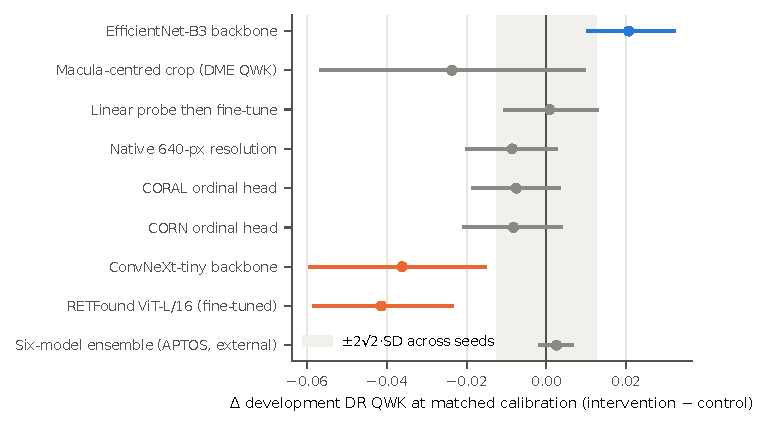
\includegraphics[width=0.8\textwidth]{figures/fig6_forest.pdf}
\caption{\textbf{Pre-registered interventions on the model.} Difference in development DR QWK
(intervention minus control) under the matched decision rule with 95\% paired-bootstrap intervals;
the macula-centred crop was registered on the DME head and the ensemble on the external set. The
grey band is $\pm2\sqrt{2}$ standard deviations of matched development QWK across five seeds of the
reference configuration (\pn{seeds.yardstick}). Blue, improvement confirmed; orange, interval
excludes zero in the unfavourable direction; grey, indistinguishable.}
\label{fig:forest}
\end{figure}

%% ---------------------------------------------------------------------------------------
\clearpage
\note{Supplementary Note 1. Decision rules}

Every model emits, for DR, four logits whose sigmoids estimate $P(y>k)$, $k=0,\dots,3$ (cumulative
head and CORAL), or conditional probabilities $P(y>k\mid y>k-1)$ that are chained by cumulative
product (CORN). From these the expected grade $s=\sum_k P(y>k)$ is computed.

\begin{description}
\item[R1 (shipped).] Grade $=\#\{k: P(y>k)>0.5\}$ after enforcing monotonicity by a running minimum.
\item[R2 (development QWK cut-points).] Four ordered cut-points on $s$ maximising QWK on the
development out-of-fold predictions, by coordinate ascent over 60 candidate values per cut-point
(8 rounds), applied unchanged externally.
\item[R3 (R2 with a referral constraint).] R2 with the grade-1/2 cut-point replaced by the largest
value that keeps development referable sensitivity at or above 0.90.
\item[R4 and R4m (external, diagnostic).] The same search on the external labels (80 candidates),
with the external set split at random into two halves (seed 0); cut-points fitted on one half are
applied to the other. R4 maximises QWK, R4m macro-averaged recall.
\item[R5 (EM prior adaptation).] Class probabilities $\pi_k(x)$ are derived from the monotone
cumulative outputs ($\pi_0=1-p_0$, $\pi_k=p_{k-1}-p_k$, $\pi_4=p_3$), clipped and renormalised.
The source prior is the mean development out-of-fold class probability; the target prior is
estimated on the unlabelled external images by the EM procedure of Saerens \emph{et al.}; posteriors
are reweighted by the ratio of the priors and decoded by argmax.
\item[R5b (black-box shift estimation).] Importance weights $w=C^{-1}\mu$, with $C$ the development
confusion matrix of R1 and $\mu$ the external distribution of R1 predictions (negative weights set
to zero); posteriors reweighted and decoded as for R5.
\end{description}

R4/R4m use external labels and are never reported as performance. Changing the development grid
from 60 to 80 values changes the reference model's matched development QWK by \pn{grid.effect}; 60 is
used for all development quantities because it reproduces the archived matched comparisons exactly.
Argmax decoding of the class probabilities derived from cumulative outputs never produced a mild
prediction for R5 on APTOS or DDR, which limits what prior adaptation can do for the mild grade
whatever the prior estimate.

%% ---------------------------------------------------------------------------------------
\note{Supplementary Note 2. Macular oedema: a supervision ceiling and an underivable grade}

No intervention moved the three-grade DME head. A crop centred on the fovea by a localiser validated
before use (median error \pn{fovea.median} disc diameters), which encodes the clinical definition of
the grade, changed DME QWK by \pn{iv.macula.diff} \pn{iv.macula.ci}. Only \pn{dme.n1} of the
\pn{n.idrid} three-grade images (\pn{dme.mid.pct}\%) carry the middle grade, and a deployed commercial
system reached a DME sensitivity of \pn{lit.p12.dme.sens}\% ($\kappa$ \pn{lit.p12.dme.kappa}) on the
same images on which its referable-DR $\kappa$ was \pn{lit.p12.dr.kappa} (Duggal \emph{et al.}, JMIR
Med Inform 2025).

IDRiD defines its DME risk grade by the distance from the fovea to the nearest hard exudate: grade
0, no exudate; grade 1, exudates more than one disc diameter from the fovea; grade 2, within one disc
diameter. Because the definition is geometric, a grade derived from the pixel-level exudate masks
that IDRiD releases for 81 images, with its fovea and optic-disc annotations, should reproduce the
expert grade if the grade is what its definition says; the test was committed before it was computed
(Table S1). Of the 81 images, \pn{parta.n} could be linked to their grading-set copies (minimum pixel
correlation 0.9999). The derived grade matched the expert grade in \pn{parta.exact}\% of images,
against \pn{parta.constant}\% for a constant predictor, because almost every segmentation image is
grade 2. On the \pn{parta.informative} informative images (expert grade 0 or 1) the derivation failed
twice, each time on a single small exudate lying just inside the threshold, so the pre-specified gate
failed and no derived DME labels were used.

%% ---------------------------------------------------------------------------------------
\note{Supplementary Note 3. A per-grade verdict that depends on the cut-point procedure}

A development source control (E12) compared runs identical except for whether Messidor-2 images
came from the default or the native-resolution files, on the 953 development images both could use.
Moderate recall, native minus default, under four ways of setting both arms' cut-points:

\begin{center}\small
\begin{tabular}{@{}lc@{}}
\toprule
Cut-points for both arms & Moderate recall difference (points) [95\% CI] \\
\midrule
Shipped (0.5) & \pn{rec.e12.shipped} \pn{rec.e12.shippedci} \\
Fitted on all rows (in-sample) & \pn{rec.e12.insample} \pn{rec.e12.insampleci} \\
Random two-fold cross-fit, grid 80 & \pn{rec.e12.randomhalf} \pn{rec.e12.randomhalfci} \\
Fold-wise cross-fit, grid 60 (development standard) & \pn{rec.e12.matched} \pn{rec.e12.matchedci} \\
\bottomrule
\end{tabular}
\end{center}

The originally archived value, cited in the project as a difference that \emph{survived} matched
cut-points, is reproduced by the random-half procedure; under the fold-wise procedure used for every
other development comparison it dissolves. A matched-decision-rule claim must therefore name its
fitting procedure, and per-grade claims should be reported under at least two.

%% ---------------------------------------------------------------------------------------
\note{Supplementary Note 4. Correction of an archived ordinal-head comparison}

Regenerating every development number from the archived per-image logits with independent code
reproduced each archived matched QWK exactly except one. The archived comparison of the CORN head
against the reference reported \pn{corn.archived.diff} \pn{corn.archived.ci}, with matched QWK
\pn{corn.archived.qwk} for CORN. The archived script had decoded CORN's conditional logits as if they
were cumulative; decoding them by cumulative product gives \pn{dev.e22corn.matched} and a difference
of \pn{iv.corn.diff} \pn{iv.corn.ci}, indistinguishable from the reference. The pre-registered
verdict (no improvement) is unchanged; the claim that CORN is worse is withdrawn.

%% ---------------------------------------------------------------------------------------
\note{Supplementary Note 5. Seed variation (O1--O3)}

The reference configuration was trained with \pn{seeds.n} seeds on identical data, split and recipe
(O1, the noise floor): matched development QWK \pn{seeds.dev.lo}--\pn{seeds.dev.hi} (s.d.\
\pn{seeds.dev.sd}); APTOS QWK at the shipped rule \pn{seeds.aptos.qwklo}--\pn{seeds.aptos.qwkhi}
(s.d.\ \pn{seeds.aptos.sd}). Of \pn{seeds.aptos.ntests} per-grade recall differences between pairs
of seeds on APTOS, \pn{seeds.aptos.sigR1} had an interval excluding zero at the shipped rule (largest
\pn{seeds.aptos.maxR1} points) and \pn{seeds.aptos.sigR4} with refitted cut-points (O2
\pn{seeds.o2}); on DDR \pn{seeds.ddr.sigR1} and \pn{seeds.ddr.sigR4} of \pn{seeds.ddr.ntests}. Mild
recall on APTOS was \pn{seeds.aptos.mildR1.lo}--\pn{seeds.aptos.mildR1.hi}\% at the shipped rule and
\pn{seeds.aptos.mildR4m.lo}--\pn{seeds.aptos.mildR4m.hi}\% under R4m in every seed (O3 \pn{seeds.o3}).

\begin{table}[h]
\caption{\textbf{Seed variation of the reference configuration (O1--O3).} Five independent training seeds of E08 (identical data, split and recipe).}\label{tab:s6}
\centering\scriptsize
\begin{tabular}{@{}lrrrrr@{}}
\toprule
Seed & Dev QWK (matched) & APTOS QWK (R1) & APTOS mild R1 (\%) & APTOS mild R4m (\%) & DDR QWK (R1) \\
\midrule
E08 & 0.8646 & 0.897 & 5.9 & 70.8 & 0.733 \\
S1E08 & 0.8685 & 0.896 & 5.4 & 70.3 & 0.717 \\
S2E08 & 0.8714 & 0.895 & 6.2 & 72.7 & 0.704 \\
S3E08 & 0.8764 & 0.890 & 5.9 & 72.4 & 0.728 \\
S4E08 & 0.8692 & 0.894 & 5.9 & 63.8 & 0.713 \\
\bottomrule
\end{tabular}
\end{table}


%% ---------------------------------------------------------------------------------------
\clearpage
\note{Supplementary Note 6. Reverse direction (O4--O6)}

The reference recipe was trained on APTOS 2019 (own frozen 5-fold split, near-duplicates grouped)
and evaluated on Messidor-2 and IDRiD. Matched out-of-fold QWK on APTOS was \pn{rev.dev.qwk}. On
Messidor-2 at the shipped rule mild recall was \pn{rev.m2.R1.mild}\% (O4 \pn{rev.o4}); external
cut-points raised it to \pn{rev.m2.R4m.mild}\% (O5 \pn{rev.o5}). The mean predicted-minus-true grade
at the shipped rule was \pn{rev.m2.R1.mean} (O6, under-grading, \pn{rev.o6}).

\begin{table}[h]
\caption{\textbf{Reverse direction (O4--O6).} The reference recipe trained on APTOS 2019 and evaluated on Messidor-2 and IDRiD.}\label{tab:s7}
\centering\scriptsize
\begin{tabular}{@{}llrrrrrr@{}}
\toprule
Corpus & Rule & QWK & Mild recall (\%) & Mild F1 & Sens. (\%) & Spec. (\%) & Pred.$-$true grade \\
\midrule
Messidor-2 & R1 & 0.715 & 34.4 & 0.276 & 43.5 & 99.2 & $-$0.26 \\
 & R2 & 0.705 & 16.3 & 0.168 & 47.3 & 98.9 & $-$0.32 \\
 & R3 & 0.679 & 17.0 & 0.155 & 34.4 & 99.7 & $-$0.36 \\
 & R4 & 0.779 & 25.9 & 0.273 & 77.9 & 93.8 & $-$0.02 \\
 & R4m & 0.755 & 44.4 & 0.325 & 82.7 & 91.7 & +0.16 \\
\addlinespace
IDRiD & R1 & 0.807 & 64.0 & 0.239 & 81.7 & 96.9 & $-$0.24 \\
 & R2 & 0.827 & 36.0 & 0.200 & 85.4 & 95.3 & $-$0.23 \\
 & R3 & 0.810 & 44.0 & 0.173 & 75.5 & 97.9 & $-$0.31 \\
 & R4 & 0.841 & 28.0 & 0.200 & 88.2 & 92.7 & $-$0.04 \\
 & R4m & 0.828 & 56.0 & 0.231 & 88.9 & 92.2 & +0.08 \\
\addlinespace
\bottomrule
\end{tabular}
\end{table}


%% ---------------------------------------------------------------------------------------
\clearpage
\note{Supplementary Note 7. Content-overlap audit}

Every image of the development pool, APTOS, DDR and EyePACS was reduced to a 256-bit difference hash
after the training crop. In this project's data, re-encodings of one photograph lie within 8 bits of
each other and distinct photographs at least 28 bits apart; all pairs within \pn{ov.bits} bits were
counted and every pair within 8 bits was archived.

\emph{Development pool and external sets.} No development image lay within 8 bits of any APTOS or DDR
image (closest pairs \pn{ov.devvsAPTOS.mind} and \pn{ov.devvsDDR.mind} bits).

\emph{EyePACS and external sets.} No external image was hash-identical to an EyePACS image.
\pn{ov.EyePACSvsAPTOS.le8} APTOS--EyePACS pairs (\pn{ov.aptos.flagged} APTOS images) and
\pn{ov.EyePACSvsDDR.le8} DDR--EyePACS pairs (\pn{ov.ddr.flagged} DDR images) lay within 8 bits, the
closest at \pn{ov.EyePACSvsAPTOS.mind} and \pn{ov.EyePACSvsDDR.mind} bits; their distances rise
towards the threshold rather than peaking at zero, as expected of hash collisions between dark,
low-contrast photographs. Removing every flagged image changed no model's shipped-rule referable
sensitivity, mild recall, QWK or referral AUC by more than \pn{ov.ddr.maxchange} percentage points on
DDR and \pn{ov.aptos.maxchange} on APTOS.

\emph{Within corpora.} The development pool contains \pn{ov.devwithin.exact} hash-identical pairs,
\pn{ov.crossfold} of which straddle two folds of the frozen split (\pn{dup.nimg} images, missed when the
split was built); removing them changes every model's matched development QWK by at most
\pn{dup.maxdiff}. APTOS and DDR contain \pn{ov.APTOSwithin.exact} and \pn{ov.DDRwithin.exact}
hash-identical pairs.

\begin{table}[h]
\caption{\textbf{Content-overlap audit.} Pairs of images across corpora whose 256-bit difference hashes lie within the stated Hamming distance.}\label{tab:s8}
\centering\scriptsize
\begin{tabular}{@{}lrrrr@{}}
\toprule
Corpus pair & Images & Pairs $\leq$16 bits & $\leq$8 bits & 0 bits \\
\midrule
within Development pool & 2,260 & 29 & 10 & 10 \\
Development pool vs APTOS & 2,260 / 3,662 & 47 & 0 & 0 \\
within APTOS & 3,662 & 1,355 & 149 & 148 \\
Development pool vs DDR & 2,260 / 12,522 & 14 & 0 & 0 \\
within DDR & 12,522 & 23,021 & 265 & 120 \\
APTOS vs DDR & 3,662 / 12,522 & 1,361 & 1 & 0 \\
EyePACS vs APTOS & 35,126 / 3,662 & 10,086 & 18 & 0 \\
EyePACS vs DDR & 35,126 / 12,522 & 267,402 & 2,304 & 0 \\
EyePACS vs Development pool & 35,126 / 2,260 & 178 & 0 & 0 \\
\multicolumn{5}{@{}l}{Threshold 16 bits; development pairs split across folds: 7} \\
\bottomrule
\end{tabular}
\end{table}


%% ---------------------------------------------------------------------------------------
\clearpage
\note{Full decision-rule matrices}
\begin{table}[h]
\caption{\textbf{Full decision-rule matrix, APTOS.} QWK, accuracy, per-grade recall (\%) and referable-DR sensitivity/specificity (\%) of every model under every rule. R4/R4m are fitted on the external labels by two-fold cross-fitting and are diagnostic bounds, not performance.}\label{tab:rules_aptos}
\centering\scriptsize
\begin{tabular}{@{}llrrrrrrrrr@{}}
\toprule
Model & Rule & QWK & Acc. & No DR & Mild & Mod. & Sev. & PDR & Sens. & Spec. \\
\midrule
E08 & R1 & 0.897 & 73.5 & 97.0 & 5.9 & 64.2 & 64.2 & 52.2 & 99.5 & 84.3 \\
 & R2 & 0.883 & 68.2 & 98.3 & 8.9 & 39.0 & 56.0 & 65.4 & 99.1 & 85.1 \\
 & R3 & 0.882 & 67.9 & 98.3 & 4.6 & 39.2 & 56.0 & 65.4 & 99.3 & 84.2 \\
 & R4 & 0.904 & 78.2 & 98.8 & 18.1 & 77.9 & 49.7 & 47.8 & 96.6 & 87.0 \\
 & R4m & 0.886 & 75.2 & 96.6 & 70.8 & 49.0 & 47.2 & 56.3 & 80.4 & 95.4 \\
\addlinespace
E09 & R1 & 0.879 & 69.3 & 88.5 & 4.3 & 66.8 & 62.7 & 45.8 & 99.3 & 84.1 \\
 & R2 & 0.863 & 62.0 & 88.5 & 22.7 & 30.3 & 62.2 & 56.6 & 96.3 & 87.4 \\
 & R3 & 0.847 & 61.0 & 88.5 & 1.4 & 34.3 & 62.2 & 56.6 & 99.7 & 79.7 \\
 & R4 & 0.898 & 76.7 & 98.6 & 10.0 & 75.5 & 48.7 & 48.5 & 98.6 & 85.9 \\
 & R4m & 0.886 & 75.6 & 97.8 & 61.6 & 53.6 & 50.3 & 48.5 & 81.1 & 94.7 \\
\addlinespace
E10 & R1 & 0.887 & 70.8 & 94.4 & 4.3 & 59.9 & 72.5 & 45.8 & 99.0 & 84.2 \\
 & R2 & 0.885 & 70.1 & 98.1 & 7.0 & 50.3 & 42.0 & 63.1 & 98.8 & 84.7 \\
 & R3 & 0.884 & 69.8 & 98.1 & 3.2 & 50.8 & 42.0 & 63.1 & 99.2 & 84.0 \\
 & R4 & 0.898 & 76.8 & 98.0 & 13.5 & 75.5 & 50.3 & 49.2 & 97.2 & 85.9 \\
 & R4m & 0.876 & 73.0 & 97.8 & 77.8 & 36.6 & 50.8 & 52.5 & 72.6 & 97.0 \\
\addlinespace
E11FULL & R1 & 0.903 & 74.9 & 98.1 & 4.9 & 65.6 & 63.2 & 60.3 & 99.3 & 84.3 \\
 & R2 & 0.900 & 72.9 & 98.9 & 7.6 & 54.5 & 63.2 & 64.1 & 99.0 & 84.9 \\
 & R3 & 0.900 & 72.8 & 98.9 & 7.0 & 54.6 & 63.2 & 64.1 & 99.1 & 84.8 \\
 & R4 & 0.907 & 79.1 & 98.6 & 16.8 & 81.8 & 39.4 & 54.6 & 96.5 & 86.6 \\
 & R4m & 0.890 & 73.4 & 97.6 & 75.1 & 37.3 & 51.3 & 59.7 & 75.3 & 96.4 \\
\addlinespace
E14MAC & R1 & 0.880 & 68.7 & 95.5 & 5.7 & 53.9 & 72.5 & 31.9 & 98.7 & 84.3 \\
 & R2 & 0.879 & 67.2 & 98.6 & 5.7 & 39.6 & 72.0 & 42.7 & 98.3 & 84.7 \\
 & R3 & 0.877 & 67.1 & 98.6 & 1.4 & 40.9 & 72.0 & 42.7 & 99.2 & 83.6 \\
 & R4 & 0.889 & 74.6 & 98.9 & 10.3 & 69.0 & 52.8 & 40.3 & 97.6 & 85.7 \\
 & R4m & 0.857 & 71.5 & 97.4 & 75.7 & 35.7 & 44.0 & 46.8 & 71.2 & 96.6 \\
\addlinespace
E15LPFT & R1 & 0.874 & 65.3 & 89.6 & 5.1 & 45.1 & 70.5 & 57.6 & 99.2 & 84.2 \\
 & R2 & 0.880 & 69.2 & 97.2 & 10.3 & 43.5 & 57.0 & 66.1 & 98.3 & 85.3 \\
 & R3 & 0.878 & 68.9 & 97.2 & 5.1 & 44.5 & 57.0 & 66.1 & 99.1 & 84.2 \\
 & R4 & 0.898 & 77.3 & 98.6 & 11.9 & 77.5 & 44.6 & 49.2 & 97.3 & 86.0 \\
 & R4m & 0.878 & 75.5 & 97.7 & 70.3 & 49.3 & 34.2 & 61.4 & 78.5 & 96.0 \\
\addlinespace
E17NAT & R1 & 0.891 & 71.1 & 96.1 & 5.9 & 56.8 & 72.0 & 47.8 & 99.2 & 84.6 \\
 & R2 & 0.872 & 65.5 & 97.3 & 9.5 & 32.2 & 48.2 & 64.7 & 99.0 & 85.0 \\
 & R3 & 0.870 & 64.9 & 97.3 & 3.2 & 32.6 & 48.2 & 64.7 & 99.4 & 83.7 \\
 & R4 & 0.894 & 76.5 & 99.1 & 16.2 & 72.0 & 48.7 & 47.8 & 96.3 & 86.9 \\
 & R4m & 0.874 & 73.6 & 97.7 & 72.7 & 41.7 & 50.3 & 51.2 & 74.0 & 96.3 \\
\addlinespace
E20CORAL & R1 & 0.879 & 66.3 & 96.1 & 14.3 & 39.1 & 64.8 & 42.4 & 98.2 & 85.3 \\
 & R2 & 0.869 & 65.7 & 98.1 & 13.8 & 33.6 & 47.7 & 53.2 & 98.2 & 85.4 \\
 & R3 & 0.867 & 65.2 & 98.1 & 4.1 & 35.2 & 47.7 & 53.2 & 99.4 & 83.3 \\
 & R4 & 0.887 & 75.2 & 97.8 & 15.7 & 73.8 & 35.8 & 42.4 & 97.1 & 85.7 \\
 & R4m & 0.872 & 73.1 & 97.3 & 72.4 & 45.4 & 48.2 & 35.6 & 79.4 & 95.5 \\
\addlinespace
E22CORN & R1 & 0.892 & 72.7 & 97.6 & 1.6 & 62.3 & 71.0 & 45.8 & 99.3 & 83.9 \\
 & R2 & 0.889 & 69.3 & 97.0 & 10.8 & 47.3 & 76.2 & 43.1 & 98.4 & 85.3 \\
 & R3 & 0.887 & 69.1 & 97.0 & 5.4 & 48.5 & 76.2 & 43.1 & 99.3 & 84.0 \\
 & R4 & 0.896 & 77.2 & 98.2 & 14.6 & 76.3 & 54.4 & 44.7 & 96.9 & 86.4 \\
 & R4m & 0.875 & 75.0 & 96.8 & 77.0 & 48.9 & 43.0 & 47.8 & 74.1 & 96.7 \\
\addlinespace
E21CNXA & R1 & 0.862 & 62.9 & 84.7 & 8.9 & 48.5 & 69.4 & 41.7 & 98.7 & 84.5 \\
 & R2 & 0.860 & 62.0 & 96.0 & 13.5 & 21.4 & 62.7 & 52.2 & 97.5 & 85.8 \\
 & R3 & 0.855 & 61.3 & 96.0 & 1.4 & 23.4 & 62.7 & 52.2 & 99.2 & 82.3 \\
 & R4 & 0.890 & 76.1 & 97.8 & 18.6 & 74.4 & 51.3 & 37.3 & 96.8 & 87.1 \\
 & R4m & 0.873 & 74.3 & 98.0 & 67.0 & 48.3 & 51.8 & 41.0 & 79.6 & 95.3 \\
\bottomrule
\end{tabular}
\end{table}

\clearpage
\begin{table}[h]
\caption{\textbf{Full decision-rule matrix, DDR.} QWK, accuracy, per-grade recall (\%) and referable-DR sensitivity/specificity (\%) of every model under every rule. R4/R4m are fitted on the external labels by two-fold cross-fitting and are diagnostic bounds, not performance.}\label{tab:rules_ddr}
\centering\scriptsize
\begin{tabular}{@{}llrrrrrrrrr@{}}
\toprule
Model & Rule & QWK & Acc. & No DR & Mild & Mod. & Sev. & PDR & Sens. & Spec. \\
\midrule
E08 & R1 & 0.733 & 73.7 & 97.7 & 33.3 & 51.2 & 58.5 & 50.3 & 65.5 & 98.7 \\
 & R2 & 0.734 & 68.9 & 98.8 & 22.1 & 38.2 & 53.4 & 50.3 & 62.5 & 99.0 \\
 & R3 & 0.742 & 70.5 & 98.8 & 17.5 & 43.4 & 53.4 & 50.3 & 67.1 & 98.3 \\
 & R4 & 0.805 & 69.8 & 86.2 & 25.2 & 57.8 & 57.2 & 49.2 & 80.8 & 93.2 \\
 & R4m & 0.787 & 67.0 & 83.6 & 59.8 & 49.8 & 55.9 & 45.3 & 66.8 & 98.4 \\
\addlinespace
E09 & R1 & 0.697 & 68.8 & 93.5 & 20.5 & 46.4 & 54.7 & 46.3 & 63.9 & 97.3 \\
 & R2 & 0.708 & 58.6 & 92.0 & 31.7 & 18.1 & 56.8 & 47.0 & 50.4 & 99.2 \\
 & R3 & 0.733 & 66.5 & 92.0 & 11.7 & 43.0 & 56.8 & 47.0 & 72.1 & 93.4 \\
 & R4 & 0.753 & 60.7 & 77.1 & 38.4 & 43.6 & 48.3 & 50.4 & 70.9 & 94.1 \\
 & R4m & 0.744 & 57.3 & 71.6 & 51.6 & 41.2 & 61.0 & 41.4 & 64.9 & 96.9 \\
\addlinespace
E10 & R1 & 0.737 & 70.5 & 96.1 & 43.7 & 44.8 & 59.3 & 42.7 & 62.8 & 98.2 \\
 & R2 & 0.740 & 69.3 & 97.4 & 27.1 & 41.9 & 41.9 & 47.8 & 63.4 & 98.2 \\
 & R3 & 0.748 & 71.1 & 97.4 & 21.6 & 47.6 & 41.9 & 47.8 & 68.3 & 97.4 \\
 & R4 & 0.793 & 67.2 & 85.1 & 23.5 & 53.1 & 67.4 & 43.3 & 80.4 & 92.6 \\
 & R4m & 0.775 & 63.4 & 83.0 & 57.9 & 40.9 & 58.5 & 43.4 & 66.7 & 97.6 \\
\addlinespace
E11FULL & R1 & 0.755 & 76.1 & 98.2 & 29.8 & 56.7 & 55.5 & 56.1 & 70.3 & 98.7 \\
 & R2 & 0.756 & 72.5 & 98.9 & 22.1 & 46.9 & 56.4 & 55.6 & 65.2 & 99.0 \\
 & R3 & 0.757 & 72.6 & 98.9 & 21.4 & 47.4 & 56.4 & 55.6 & 65.6 & 98.9 \\
 & R4 & 0.813 & 72.8 & 89.2 & 24.6 & 60.2 & 60.6 & 58.4 & 81.2 & 94.2 \\
 & R4m & 0.799 & 66.7 & 84.2 & 58.7 & 46.3 & 64.8 & 53.1 & 69.4 & 98.4 \\
\addlinespace
E14MAC & R1 & 0.736 & 70.2 & 96.3 & 42.1 & 43.7 & 71.2 & 39.6 & 61.7 & 98.9 \\
 & R2 & 0.729 & 68.1 & 98.6 & 19.5 & 37.1 & 62.7 & 45.2 & 62.5 & 98.8 \\
 & R3 & 0.740 & 70.4 & 98.6 & 10.2 & 44.9 & 62.7 & 45.2 & 69.4 & 97.4 \\
 & R4 & 0.793 & 67.8 & 84.7 & 24.0 & 55.2 & 61.9 & 45.5 & 80.1 & 93.1 \\
 & R4m & 0.776 & 64.8 & 84.4 & 57.1 & 43.8 & 68.2 & 38.4 & 65.6 & 98.3 \\
\addlinespace
E15LPFT & R1 & 0.764 & 69.9 & 92.5 & 45.2 & 43.7 & 63.1 & 62.3 & 66.1 & 98.3 \\
 & R2 & 0.743 & 68.9 & 97.5 & 21.4 & 38.2 & 51.7 & 60.0 & 62.2 & 98.8 \\
 & R3 & 0.753 & 71.2 & 97.5 & 16.5 & 45.4 & 51.7 & 60.0 & 68.4 & 97.9 \\
 & R4 & 0.794 & 67.5 & 84.6 & 35.2 & 52.0 & 66.5 & 48.6 & 76.8 & 94.5 \\
 & R4m & 0.786 & 64.4 & 81.0 & 57.6 & 44.5 & 61.0 & 54.0 & 67.6 & 97.9 \\
\addlinespace
E17NAT & R1 & 0.743 & 71.5 & 96.9 & 38.9 & 46.4 & 58.9 & 45.5 & 64.6 & 98.2 \\
 & R2 & 0.765 & 66.9 & 96.1 & 33.8 & 35.0 & 54.7 & 48.5 & 65.2 & 98.3 \\
 & R3 & 0.772 & 68.9 & 96.1 & 26.5 & 41.6 & 54.7 & 48.5 & 71.0 & 97.0 \\
 & R4 & 0.801 & 67.5 & 85.7 & 31.4 & 51.8 & 55.5 & 48.2 & 79.4 & 93.4 \\
 & R4m & 0.789 & 63.4 & 83.3 & 62.1 & 40.4 & 63.6 & 41.1 & 67.5 & 97.8 \\
\addlinespace
E20CORAL & R1 & 0.740 & 65.2 & 93.8 & 37.8 & 36.0 & 59.3 & 33.1 & 58.9 & 98.5 \\
 & R2 & 0.728 & 65.6 & 96.2 & 24.9 & 33.8 & 50.8 & 43.8 & 58.9 & 98.5 \\
 & R3 & 0.743 & 69.6 & 96.2 & 14.4 & 46.5 & 50.8 & 43.8 & 69.7 & 96.6 \\
 & R4 & 0.778 & 64.2 & 82.9 & 37.1 & 46.4 & 57.6 & 43.5 & 75.1 & 94.1 \\
 & R4m & 0.768 & 60.6 & 81.0 & 58.7 & 37.1 & 64.4 & 35.5 & 65.6 & 97.7 \\
\addlinespace
E22CORN & R1 & 0.699 & 72.4 & 98.7 & 25.9 & 49.1 & 56.4 & 42.5 & 63.8 & 98.6 \\
 & R2 & 0.707 & 66.5 & 98.0 & 32.4 & 34.7 & 64.0 & 30.0 & 54.7 & 99.3 \\
 & R3 & 0.730 & 70.2 & 98.0 & 24.0 & 46.3 & 64.0 & 30.0 & 65.0 & 98.3 \\
 & R4 & 0.785 & 67.4 & 85.2 & 22.7 & 54.5 & 56.4 & 41.9 & 79.4 & 92.8 \\
 & R4m & 0.766 & 63.6 & 85.9 & 56.5 & 39.1 & 63.1 & 36.3 & 63.2 & 98.6 \\
\addlinespace
E21CNXA & R1 & 0.710 & 65.4 & 88.0 & 34.9 & 45.0 & 51.7 & 34.7 & 62.6 & 98.4 \\
 & R2 & 0.701 & 62.1 & 94.9 & 23.8 & 26.3 & 53.8 & 40.4 & 55.1 & 99.2 \\
 & R3 & 0.726 & 67.8 & 94.9 & 8.7 & 44.5 & 53.8 & 40.4 & 71.3 & 95.8 \\
 & R4 & 0.747 & 58.7 & 78.5 & 41.4 & 37.3 & 56.4 & 40.3 & 70.0 & 96.3 \\
 & R4m & 0.738 & 56.9 & 70.5 & 53.5 & 43.0 & 59.3 & 32.5 & 67.4 & 97.3 \\
\bottomrule
\end{tabular}
\end{table}

\clearpage
\begin{table}[h]
\caption{\textbf{Full decision-rule matrix, DeepDRiD.} QWK, accuracy, per-grade recall (\%) and referable-DR sensitivity/specificity (\%) of every model under every rule. R4/R4m are fitted on the external labels by two-fold cross-fitting and are diagnostic bounds, not performance.}\label{tab:rules_deepdrid}
\centering\scriptsize
\begin{tabular}{@{}llrrrrrrrrr@{}}
\toprule
Model & Rule & QWK & Acc. & No DR & Mild & Mod. & Sev. & PDR & Sens. & Spec. \\
\midrule
E08 & R1 & 0.792 & 64.3 & 90.8 & 19.8 & 75.4 & 19.8 & 37.5 & 86.6 & 93.9 \\
 & R2 & 0.812 & 64.0 & 93.5 & 10.8 & 58.5 & 35.9 & 37.5 & 83.7 & 94.7 \\
 & R3 & 0.815 & 64.5 & 93.5 & 6.3 & 63.3 & 35.9 & 37.5 & 86.6 & 93.4 \\
 & R4 & 0.833 & 60.1 & 80.6 & 33.8 & 49.5 & 44.1 & 33.0 & 86.9 & 93.0 \\
 & R4m & 0.818 & 61.5 & 73.0 & 40.5 & 64.1 & 58.2 & 10.7 & 87.0 & 92.4 \\
\addlinespace
E09 & R1 & 0.747 & 60.8 & 92.3 & 10.8 & 57.3 & 22.9 & 34.8 & 77.8 & 95.1 \\
 & R2 & 0.757 & 57.2 & 89.6 & 22.5 & 23.9 & 39.5 & 35.7 & 63.1 & 97.9 \\
 & R3 & 0.777 & 61.6 & 89.6 & 7.2 & 54.3 & 39.5 & 35.7 & 83.1 & 90.4 \\
 & R4 & 0.793 & 57.9 & 81.2 & 31.5 & 28.1 & 55.9 & 32.1 & 76.5 & 95.2 \\
 & R4m & 0.781 & 57.0 & 75.3 & 32.0 & 46.7 & 45.5 & 29.5 & 77.1 & 93.1 \\
\addlinespace
E10 & R1 & 0.797 & 63.4 & 87.9 & 32.0 & 66.8 & 24.6 & 37.5 & 83.8 & 93.9 \\
 & R2 & 0.808 & 63.4 & 90.6 & 18.5 & 62.8 & 29.9 & 39.3 & 83.9 & 93.9 \\
 & R3 & 0.813 & 63.7 & 90.6 & 12.6 & 67.6 & 29.9 & 39.3 & 87.7 & 92.0 \\
 & R4 & 0.820 & 59.7 & 78.7 & 35.6 & 54.3 & 38.1 & 40.2 & 86.7 & 92.3 \\
 & R4m & 0.806 & 56.5 & 63.2 & 55.4 & 54.8 & 51.1 & 27.7 & 83.8 & 93.9 \\
\addlinespace
E11FULL & R1 & 0.819 & 66.5 & 90.7 & 23.0 & 81.7 & 19.8 & 48.2 & 90.3 & 92.3 \\
 & R2 & 0.828 & 65.5 & 91.6 & 18.9 & 71.9 & 26.3 & 45.5 & 87.6 & 93.1 \\
 & R3 & 0.830 & 65.5 & 91.6 & 18.9 & 72.4 & 26.3 & 45.5 & 88.1 & 93.1 \\
 & R4 & 0.844 & 66.3 & 83.2 & 31.5 & 65.6 & 57.9 & 26.8 & 91.4 & 91.1 \\
 & R4m & 0.839 & 61.8 & 79.2 & 41.0 & 65.3 & 30.8 & 45.5 & 87.8 & 93.0 \\
\addlinespace
E14MAC & R1 & 0.777 & 64.3 & 89.6 & 28.8 & 67.1 & 31.1 & 24.1 & 81.1 & 95.6 \\
 & R2 & 0.788 & 64.8 & 94.3 & 11.3 & 58.5 & 41.8 & 24.1 & 81.7 & 95.9 \\
 & R3 & 0.791 & 65.3 & 94.3 & 5.4 & 64.6 & 41.8 & 24.1 & 86.6 & 92.7 \\
 & R4 & 0.805 & 58.6 & 80.7 & 34.2 & 39.7 & 48.0 & 26.8 & 83.0 & 94.2 \\
 & R4m & 0.797 & 59.9 & 75.9 & 40.1 & 59.5 & 42.9 & 23.2 & 84.3 & 94.0 \\
\addlinespace
E15LPFT & R1 & 0.794 & 63.9 & 88.8 & 24.8 & 62.8 & 30.5 & 48.2 & 85.1 & 92.9 \\
 & R2 & 0.799 & 63.0 & 92.3 & 11.7 & 61.3 & 27.7 & 43.8 & 83.2 & 93.8 \\
 & R3 & 0.801 & 63.6 & 92.3 & 8.6 & 65.8 & 27.7 & 43.8 & 86.1 & 92.3 \\
 & R4 & 0.822 & 62.8 & 84.0 & 26.1 & 54.0 & 48.9 & 37.5 & 87.5 & 90.7 \\
 & R4m & 0.809 & 57.8 & 73.0 & 43.7 & 57.5 & 31.9 & 44.6 & 84.6 & 92.8 \\
\addlinespace
E17NAT & R1 & 0.797 & 63.2 & 86.0 & 34.2 & 67.6 & 26.3 & 36.6 & 84.7 & 93.5 \\
 & R2 & 0.826 & 63.1 & 85.6 & 29.3 & 55.0 & 43.2 & 39.3 & 86.1 & 93.0 \\
 & R3 & 0.823 & 63.0 & 85.6 & 18.9 & 60.1 & 43.2 & 39.3 & 89.1 & 89.6 \\
 & R4 & 0.822 & 59.5 & 79.5 & 36.9 & 41.5 & 48.3 & 39.3 & 83.1 & 94.0 \\
 & R4m & 0.816 & 57.4 & 71.8 & 42.8 & 53.0 & 39.0 & 42.0 & 85.4 & 93.3 \\
\addlinespace
E20CORAL & R1 & 0.798 & 63.2 & 89.6 & 25.2 & 52.8 & 44.1 & 20.5 & 78.7 & 95.6 \\
 & R2 & 0.797 & 63.5 & 92.6 & 18.9 & 49.2 & 43.2 & 29.5 & 78.7 & 95.6 \\
 & R3 & 0.803 & 65.4 & 92.6 & 9.9 & 63.8 & 43.2 & 29.5 & 86.9 & 92.3 \\
 & R4 & 0.823 & 60.4 & 82.8 & 28.8 & 35.2 & 59.3 & 32.1 & 83.7 & 92.9 \\
 & R4m & 0.795 & 53.7 & 55.8 & 60.4 & 50.5 & 55.9 & 27.7 & 84.6 & 93.5 \\
\addlinespace
E22CORN & R1 & 0.770 & 64.8 & 91.9 & 14.9 & 73.1 & 26.0 & 35.7 & 85.2 & 92.6 \\
 & R2 & 0.794 & 65.0 & 90.2 & 23.9 & 58.3 & 45.5 & 27.7 & 78.9 & 95.7 \\
 & R3 & 0.798 & 65.8 & 90.2 & 14.9 & 67.1 & 45.5 & 27.7 & 85.1 & 91.9 \\
 & R4 & 0.818 & 62.4 & 83.0 & 37.4 & 46.5 & 51.1 & 34.8 & 82.3 & 94.2 \\
 & R4m & 0.813 & 62.2 & 75.8 & 42.3 & 59.5 & 52.8 & 29.5 & 83.0 & 93.8 \\
\addlinespace
E21CNXA & R1 & 0.778 & 61.9 & 89.3 & 24.8 & 60.1 & 27.1 & 27.7 & 80.8 & 94.6 \\
 & R2 & 0.790 & 61.6 & 92.6 & 18.5 & 38.7 & 43.2 & 33.9 & 75.8 & 96.4 \\
 & R3 & 0.798 & 63.6 & 92.6 & 7.7 & 55.0 & 43.2 & 33.9 & 86.5 & 91.5 \\
 & R4 & 0.811 & 58.5 & 80.7 & 27.5 & 39.2 & 51.7 & 27.7 & 86.6 & 91.0 \\
 & R4m & 0.796 & 60.0 & 72.2 & 44.1 & 56.0 & 58.5 & 10.7 & 82.9 & 93.6 \\
\bottomrule
\end{tabular}
\end{table}

\clearpage
\begin{table}[h]
\caption{\textbf{Full decision-rule matrix, SUSTech.} QWK, accuracy, per-grade recall (\%) and referable-DR sensitivity/specificity (\%) of every model under every rule. R4/R4m are fitted on the external labels by two-fold cross-fitting and are diagnostic bounds, not performance.}\label{tab:rules_sustech}
\centering\scriptsize
\begin{tabular}{@{}llrrrrrrrrr@{}}
\toprule
Model & Rule & QWK & Acc. & No DR & Mild & Mod. & Sev. & PDR & Sens. & Spec. \\
\midrule
E08 & R1 & 0.923 & 82.0 & 96.4 & 33.3 & 64.7 & 94.5 & 39.7 & 99.0 & 97.9 \\
 & R2 & 0.904 & 74.2 & 97.5 & 25.0 & 43.0 & 53.4 & 63.8 & 98.2 & 98.3 \\
 & R3 & 0.902 & 74.4 & 97.5 & 12.5 & 44.4 & 53.4 & 63.8 & 99.2 & 97.3 \\
 & R4 & 0.932 & 84.4 & 98.1 & 25.0 & 73.4 & 90.4 & 22.4 & 97.4 & 98.6 \\
 & R4m & 0.900 & 76.7 & 82.9 & 79.2 & 70.4 & 82.2 & 41.4 & 92.5 & 99.5 \\
\addlinespace
E09 & R1 & 0.892 & 78.6 & 90.6 & 29.2 & 64.9 & 87.7 & 43.1 & 99.2 & 93.9 \\
 & R2 & 0.890 & 69.5 & 88.7 & 58.3 & 37.8 & 74.0 & 58.6 & 97.4 & 98.6 \\
 & R3 & 0.857 & 69.5 & 88.7 & 12.5 & 40.8 & 74.0 & 58.6 & 99.6 & 89.3 \\
 & R4 & 0.925 & 85.2 & 96.2 & 20.8 & 80.5 & 87.7 & 19.0 & 97.4 & 98.5 \\
 & R4m & 0.912 & 81.2 & 89.5 & 50.0 & 75.3 & 71.2 & 53.4 & 97.4 & 98.3 \\
\addlinespace
E10 & R1 & 0.929 & 80.5 & 97.8 & 50.0 & 55.3 & 97.3 & 41.4 & 98.6 & 98.8 \\
 & R2 & 0.901 & 76.2 & 99.5 & 33.3 & 50.1 & 26.0 & 67.2 & 98.2 & 98.8 \\
 & R3 & 0.903 & 76.5 & 99.5 & 33.3 & 51.0 & 26.0 & 67.2 & 99.0 & 98.8 \\
 & R4 & 0.937 & 87.5 & 99.4 & 25.0 & 84.9 & 71.2 & 20.7 & 99.2 & 98.5 \\
 & R4m & 0.918 & 81.5 & 95.7 & 75.0 & 62.2 & 84.9 & 46.6 & 90.1 & 99.7 \\
\addlinespace
E11FULL & R1 & 0.929 & 83.2 & 98.1 & 33.3 & 64.9 & 94.5 & 43.1 & 98.8 & 98.5 \\
 & R2 & 0.924 & 79.7 & 99.2 & 20.8 & 54.2 & 79.5 & 51.7 & 98.4 & 98.9 \\
 & R3 & 0.924 & 79.7 & 99.2 & 16.7 & 54.5 & 79.5 & 51.7 & 98.6 & 98.8 \\
 & R4 & 0.934 & 87.3 & 98.4 & 20.8 & 83.3 & 80.8 & 27.6 & 98.4 & 98.6 \\
 & R4m & 0.919 & 81.4 & 92.9 & 62.5 & 69.9 & 78.1 & 41.4 & 95.8 & 99.8 \\
\addlinespace
E14MAC & R1 & 0.919 & 77.3 & 95.7 & 58.3 & 51.5 & 95.9 & 24.1 & 98.2 & 99.2 \\
 & R2 & 0.916 & 75.6 & 99.7 & 20.8 & 40.5 & 86.3 & 43.1 & 98.2 & 99.1 \\
 & R3 & 0.917 & 75.5 & 99.7 & 4.2 & 41.4 & 86.3 & 43.1 & 99.0 & 98.3 \\
 & R4 & 0.928 & 84.3 & 99.2 & 20.8 & 74.0 & 78.1 & 20.7 & 97.6 & 99.1 \\
 & R4m & 0.916 & 80.0 & 89.9 & 75.0 & 71.5 & 74.0 & 36.2 & 96.6 & 99.7 \\
\addlinespace
E15LPFT & R1 & 0.910 & 75.2 & 93.2 & 41.7 & 47.9 & 82.2 & 56.9 & 98.4 & 98.2 \\
 & R2 & 0.906 & 75.8 & 98.3 & 20.8 & 44.7 & 60.3 & 70.7 & 97.4 & 98.9 \\
 & R3 & 0.902 & 76.1 & 98.3 & 8.3 & 46.3 & 60.3 & 70.7 & 98.6 & 97.4 \\
 & R4 & 0.936 & 85.2 & 98.1 & 20.8 & 77.0 & 74.0 & 37.9 & 98.0 & 98.2 \\
 & R4m & 0.920 & 79.6 & 90.6 & 75.0 & 65.2 & 75.3 & 56.9 & 95.8 & 99.7 \\
\addlinespace
E17NAT & R1 & 0.929 & 80.1 & 97.9 & 37.5 & 54.2 & 98.6 & 43.1 & 99.0 & 98.8 \\
 & R2 & 0.895 & 70.2 & 98.7 & 29.2 & 32.9 & 26.0 & 67.2 & 98.0 & 98.8 \\
 & R3 & 0.897 & 70.7 & 98.7 & 20.8 & 35.1 & 26.0 & 67.2 & 99.8 & 98.3 \\
 & R4 & 0.937 & 87.1 & 99.4 & 12.5 & 81.1 & 83.6 & 27.6 & 99.8 & 98.3 \\
 & R4m & 0.917 & 80.4 & 91.9 & 58.3 & 66.6 & 76.7 & 55.2 & 95.4 & 99.2 \\
\addlinespace
E20CORAL & R1 & 0.909 & 71.9 & 93.3 & 50.0 & 41.1 & 71.2 & 43.1 & 97.6 & 98.9 \\
 & R2 & 0.902 & 72.1 & 97.5 & 41.7 & 38.4 & 37.0 & 65.5 & 97.6 & 98.9 \\
 & R3 & 0.899 & 72.4 & 97.5 & 16.7 & 40.8 & 37.0 & 65.5 & 99.4 & 97.1 \\
 & R4 & 0.934 & 85.3 & 98.3 & 8.3 & 81.6 & 72.6 & 15.5 & 98.8 & 98.3 \\
 & R4m & 0.887 & 70.9 & 73.9 & 70.8 & 74.0 & 58.9 & 34.5 & 95.8 & 99.5 \\
\addlinespace
E22CORN & R1 & 0.920 & 82.9 & 97.6 & 16.7 & 66.3 & 91.8 & 43.1 & 99.2 & 97.1 \\
 & R2 & 0.919 & 77.4 & 96.2 & 29.2 & 50.7 & 91.8 & 43.1 & 97.6 & 98.5 \\
 & R3 & 0.919 & 77.7 & 96.2 & 12.5 & 52.6 & 91.8 & 43.1 & 99.2 & 97.3 \\
 & R4 & 0.929 & 85.6 & 97.5 & 8.3 & 81.4 & 86.3 & 13.8 & 98.0 & 98.3 \\
 & R4m & 0.906 & 78.0 & 84.8 & 70.8 & 72.6 & 71.2 & 50.0 & 95.2 & 99.5 \\
\addlinespace
E21CNXA & R1 & 0.883 & 65.3 & 77.7 & 41.7 & 46.0 & 80.8 & 43.1 & 98.8 & 98.0 \\
 & R2 & 0.889 & 65.6 & 91.9 & 37.5 & 26.0 & 49.3 & 60.3 & 98.0 & 99.1 \\
 & R3 & 0.876 & 65.9 & 91.9 & 12.5 & 28.8 & 49.3 & 60.3 & 100.0 & 94.7 \\
 & R4 & 0.926 & 83.3 & 98.4 & 4.2 & 76.2 & 76.7 & 5.2 & 98.4 & 98.8 \\
 & R4m & 0.900 & 74.2 & 88.1 & 62.5 & 58.1 & 60.3 & 46.6 & 94.4 & 99.7 \\
\bottomrule
\end{tabular}
\end{table}


\end{document}
